\documentclass[AMA,LATO1COL]{WileyNJD-v2}

\RequirePackage{ulem}
\articletype{Article Type}%

\usepackage{pgf}
\usepackage{enumitem}
\usepackage{subfiles}

\usepackage{placeins}

\usepackage{longtable}
\usepackage{makecell}

\received{01 July 2023}
% \revised{6 June 2023}
% \accepted{6 June 2023}

\raggedbottom

\newcommand\todo[1]{\textcolor{red}{#1}}

\newcommand\lowcomma{%
\settoheight{\commaheight}{\text{,}}%
\mathpunct{\adjustbox{valign=b,raise=-\commaheight}{\text{,}}}%
}

\usepackage[acronym]{glossaries}
\renewcommand{\glossarysection}[2][]{}
\makeglossaries


\begin{document}

\title{MRS-Sim: Open-Source Framework for Simulating In Vivo-like Magnetic Resonance Spectra\protect}

\author[1,2]{John LaMaster*}

\author[3]{Georg Oeltzschner}

\author[4]{Yan Li}

\authormark{J. LaMaster \textsc{et al.}}


\address[1]{\orgdiv{Munich Institute of Biomedical Engineering}, \orgname{Technical University of Munich}, \orgaddress{\state{Bavaria}, \country{Germany}}}

\address[2]{\orgdiv{School of Computation, Information, and Technology}, \orgname{Technical University of Munich}, \orgaddress{\state{Bavaria}, \country{Germany}}}

\address[3]{\orgdiv{Russel H. Morgan Department of Radiology and Radiological Sciences}, \orgname{The Johns Hopkins' University School of Medicine}, \orgaddress{\state{Maryland}, \country{USA}}}

\address[4]{\orgdiv{Department of Radiology and Biomedical Imaging}, \orgname{University of California, San Francisco}, \orgaddress{\state{California}, \country{USA}}}

\corres{John LaMaster. \\\email{john.t.lamaster@gmail.com} \\Twitter: @JohnTLaMaster}

\presentaddress{Munich Institute of Biomedical Engineering, School of Computation, Information, and Technology, Technical University of Munich in the City of Garching bei München, Boltzmannstr 11. 85748 Garching bei München, Bavaria, Germany.}

\abstract[Summary]{MRS-Sim is a powerful, open-source framework for simulating in vivo-like magnetic resonance spectroscopy data. Its modularity allows it to model the complexities of MRS data for a variety of clinical scenarios. The underlying physical equations include spectral components commonly found in linear-combination fitting routines plus some novel components. The first is a 3D $B_0$ field map simulator to model $B_0$ field inhomogeneities, ranging from slight variations to severe distortions. The second is a novel semi-parametric generator that mimics signals from poorly characterized residual water regions and baseline offset contributions. This framework can simulate everything from raw multi-coil transients to preprocessed coil-combined data. 

A repository of information has been compiled to help non-expert users with general simulations of MRS data. Simulating realistic clinical-like datasets requires appropriate ranges and distributions for the model parameters, which are best determined by analyzing the parameter estimates from fitting real clinical data. Therefore, accompanying tools within MRS-Sim allow for analyzing the range and distributions of those parameters from in vivo datasets fitted with Osprey. This allows simulations to be tailored to specific clinical datasets.

The modularity of this framework allows for easy customization of simulations to suit a variety of clinical scenarios and encourages continued community development. Using a single framework for various scenarios overcomes the inconsistent protocols in current literature. By simulating in vivo-like data, this framework can aid in many tasks in MRS, including verifying spectral fitting protocols and reproducibility analyses. The accessibility of readily available, synthetic data will also assist deep learning research for MRS, particularly in cases where clinical data is insufficient or unavailable for training and, in general, will help address reproducibility issues and make MRS research more accessible to a wider audience.\\
Word count (abstract): 295 -> 297 -> 282 words\\
Word count (*paper): 4,206 -> 5,125 -> 6,314 words\\
*Limited to intro, methods, results, and conclusions. Including auxiliary text (author info, etc.): 4,807 -> 5,757 -> 6,805 words
% \cite{Li2015}
} 

\keywords{MRS, spectroscopy, in vivo, data simulation, synthetic data, open-source}


\jnlcitation{\cname{%
\author{LaMaster J.}, 
\author{G. Oeltzschner}, and 
\author{Y. Li}} (\cyear{2022}), 
\ctitle{MRS-Sim: Open-Source Framework for Simulating Realistic In Vivo-like MR Spectroscopy Data}, \cjournal{NMR in Biomedicine}.}%, \cvol{2017;00:1--6}.}

\maketitle

\section{Introduction}\label{sec:Introduction}
Magnetic resonance spectroscopy (MRS) is a non-invasive imaging modality that provides in vivo information on the metabolic profile of tissues, enabling the evaluation of various pathologies throughout the entire body. Such an evaluation is possible by analyzing the spectra to quantify metabolite concentrations, which reflect valuable insights such as tissue composition and metabolic activity. In the brain, MRS has been extensively used to investigate a wide range of pathologies, including neurodevelopmental\cite{Augustine2008,Laccetta2022,Tomiyasu2022} and neurodegenerative diseases\cite{Gao2014,Martin2007,McKiernan2023,Oz2016}, inborn errors of metabolism\cite{Cecil2006,Gropman2020,Lai2022}, brain tumors\cite{Calvar2005,Lukas2004,Padelli2022,Nelson2003}, as well as age-related changes\cite{Forester2010,Inglese2004,Reyngoudt2012}. All of those studies are based on analyzing metabolite concentrations, or how the concentrations change. %This is only possible with accurate post-processing and quantification steps.
 
For MRS to become a widely used clinical imaging modality, among other things, it is important to ensure the precision and accuracy of MRS data processing and analysis across a wide range of data scenarios, e.g. acquisition parameters, pulse sequences, data quality regimes, pediatrics versus adult subjects, and disease-related metabolic patterns. In vivo MRS data varies drastically across these dimensions, but is usually not widely available for method development and evaluation due to data privacy restrictions. Furthermore, in vivo data lacks access to a ground truth values making it difficult to determine how reliable, sensitive, and robust the quantitative outcomes are from different MRS analysis procedures. Phantom data can be useful in developing and validating acquisition and analysis methods, but usually does not adequately reflect the complexities of in vivo spectra. %For example, phantom data does not contain broad signals from macromolecules and lipids, which are a major source of uncertainty during spectral modeling. In vivo MRS data is further affected by tissue and susceptibility heterogeneities, reflected in irregular lineshapes and artifacts.


A logical solution to these challenges is to use synthetic data which has the possibility of being simulated for any variety of experimental scenarios. The main challenge of synthetic MRS data generation is to adequately incorporate all physical phenomena underlying in vivo data. One such aspect is the adequate choice of model parameters to reflect different physiological and pathological conditions. Arguably more important is the need to capture acquisition-induced artifacts and nuisance signals commonly found in in vivo data that are difficult to reproduce in a phantom: effects of susceptibility and field inhomogeneity, macromolecule, lipid, and residual water signals, and various other artifacts. 
While many research groups now routinely use synthetic data, the underlying software, crucial data generation models, and parameter distributions are rarely made publicly available. This not only hampers systematic comparison, but also the formation of consensus best practices for synthetic data generation. 

The lack of standardized best practices is evident in literature which shows that synthetic data is simulated using physical models with a variety of complexity and spectral components.\cite{Hatami,Das2018a,Das2018,Iqbal2018a} Most of these methods begin with simulated basis functions that are assumed to have been simulated using appropriate pulse sequence parameters for the scenario of interest. These metabolite basis functions are then modulated by scaling factors that indicate their underlying concentrations. Most models then apply a simple Lorentzian lineshape.\cite{Hatami, Das2018a, Das2018} Phase offsets\cite{Das2018,Iqbal2018a} and frequency shifts\cite{Hatami} can optionally be applied. Finally, some type of broad baseline is typically added. These models are simple and do not capture the full complexity of in vivo data. Additionally, they often include non-public components such as baselines, macromolecules, and lipid signals that are either simulated in-house or extracted from private datasets, both of which prevent detailed analysis of their models.

% Many software packages\cite{Hogben2011, Landheer2021, Simpson2017,Smith1994, Soher2011, Stefan2009, Tal2020} can already accurately calculate the evolution of spin systems for arbitrary pulse sequences, enabling the generation of metabolite basis sets, which form the backbone of in vivo simulation methods. 
% These can then be assembled into arbitrarily large datasets that can approximate in vivo spectra with known ground truth values, offering a pathway to evaluate the accuracy and precision of data analysis methods.

There are a handful of software packages that claim to simulate in vivo spectra, such as FID-A\cite{Simpson2017}, GAVA\cite{Soher2007}, and VESPA\cite{Soher2023}. There is a fundamental difference between these methods and the current work though: the definition of "in vivo spectra". Generally, prior works have used this term when simulating rather idealized spectra to evaluate parameter settings to aid in developing new pulse sequences. In this work, "in vivo spectra" refers to the data that comes off a clinical scanner before post-processing and analysis begins and is meant to advance the use of synthetic data for MRS applications. While pulse sequences are necessary for the basis sets that are required for these simulations, they are left to the many software options already available. The recent update for the MARSS\cite{Landheer2021} software has added a new functionality called synMARSS that simulates synthetic spectra and incorporates many spectral artifacts. They provide an extensive user manual with equations describing their implementation; however, their source code is not available nor can it be modified like MRS-Sim.
% Previous work:
% GAVA "This application provides a convenient method for generating a priori spectral information used in parametric spectral analyses and for visual examination of the effects of difference pulse sequences and parameter settings"
% VESPA: focuses on simulating basis functions to help design pulse sequences


% The continued rise in the use of synthetic MRS data without standardization will further exacerbate this problem.


Recent years have seen a dramatic increase in the use of synthetic MRS data, primarily catalyzed by the advent of machine learning\cite{Das2017} (ML) and deep learning\cite{Gurbani2019, Hatami, Lee2019} (DL) analysis algorithms that require vast amounts of data for training and validation. 
These deep learning techniques require datasets comprising tens of thousands to hundreds of thousands of spectra to be effective, a volume of data that few centers globally possess. As a result, generating realistic, in vivo-like synthetic data is necessary to facilitate more research into these applications. Synthetic data is uniquely suited for such applications because it inherently has known ground truth values required to evaluate the accuracy and precision of the analysis methods being developed. 
% Many software packages\cite{Hogben2011, Landheer2021, Simpson2017,Smith1994, Soher2011, Stefan2009, Tal2020} can already accurately calculate the evolution of spin systems for arbitrary pulse sequences, enabling researchers to generate metabolite basis sets. These can then be assembled into arbitrarily large datasets that can approximate in vivo spectra with known ground truth values, offering a pathway to evaluate the accuracy and precision of data analysis methods.
Growing interest in training ML and DL models with synthetic data will compound the reproducibility and generalizability problems already being experienced in the traditional MRS field.\cite{Craven2022,Marjanska2021,Marjanska2022,Zollner2021} To address this challenge, it will be essential to establish standards and best practices for simulating synthetic MRS data. This will require collaboration and consensus-building among researchers, as well as the development and adoption of open-source frameworks for data generation. Unfortunately, a consensus-building effort surrounding synthetic data generation is beyond the scope of this work.  %, therefore, this work focuses an open-source generation framework is well within the scope.
% To ensure widespread adoption, these frameworks will need to be applicable across a range of MRS applications. 
% While a consensus-building effort is beyond the scope of this work, an open-source framework is not.


Therefore, this work presents
% In this work, we therefore present 
a framework for a modular synthetic data generation model. The basic model applies well-defined distributions of physical parameters commonly used in linear-combination modeling software, corresponding to amplitudes, lineshapes, phases, and frequency shifts. Furthermore, it incorporates a realistic $B_0$ map generator to simulate in vivo-like field heterogeneity conditions, and uses parameterized models to describe residual water and smooth background signal contributions. 
The software is designed to simulate spectra at any stage of acquisition: from individual coil elements to unaligned transients to fully processed spectra. These features allow researchers to benchmark new data processing methods, not just modeling algorithms, against known ground truth parameters. The framework's flexibility allows users to simulate custom-tailored datasets for a large variety of clinical scenarios. Accompanying this simulator are tools to analyze existing in vivo datasets and extract parameter distributions, which then allows for augmenting in vivo data with similar synthetic data. 
The open-source code base allows for seamless incorporation of future additions to expand the software's capabilities to include more types of spectra, spectral model components, and parameter distributions reflecting pathological metabolic signatures. This work is intended to be a community resource to provide researchers, trainees, and experts alike with access to high-quality and comparable synthetic data as a source of continuity in the field.


% The main challenge of synthetic MRS data generation is to adequately incorporate all physical phenomena underlying in vivo data. One aspect is the adequate choice of model parameters to reflect different pathological conditions. %For example, tumors have vastly different metabolic signatures than healthy tissue. 
% % More importantly, synthetic data needs 
% Arguably more important is the need to capture acquisition-induced artifacts and nuisance signals commonly found in in vivo data that are difficult to reproduce in a phantom: effects of susceptibility and field inhomogeneity, macromolecule, lipid, and residual water signals, and various other artifacts. While many research groups now routinely use synthetic data, the underlying software, crucial data generation models, and parameter distributions are rarely made publicly available. This not only hampers systematic comparison, but also the formation of consensus best practices for synthetic data generation. Literature shows that synthetic data is simulated using physical models with a variety of complexity and spectral components.\cite{Hatami,Das2018a,Das2018,Iqbal2018a} The continued rise in the use of synthetic MRS data without standardization will further exacerbate this problem.
 
% Recent work has begun to compare the impact of various spectral modeling components on metabolite quantification as well as the performance of commonly used spectral fitting models.\cite{Craven2022,Marjanska2021,Marjanska2022,Zollner2021} Currently, these comparisons show worrisome agreement of metabolite quantities between the different linear combination fitting methods. Poor agreement between fitting methods prevents any sort of meaningful comparison between studies published by different institutions that employ different fitting protocols which limits the generalizability of published quantification parameters and any conclusions drawn from them.
 
% Growing interest in training ML and DL models with synthetic data will compound the reproducibility and generalizability problems already being experienced in the traditional MRS field. To address this challenge, it is essential to establish standards and best practices for simulating MRS data. This will require collaboration and consensus-building among researchers, as well as the development and adoption of open-source frameworks for data generation. To ensure widespread adoption, these frameworks will need to be applicable across a range of MRS applications. While a consensus-building effort is beyond the scope of this work, an open-source framework is not.
 
 
% % \subsection{Contribution}\label{subsec:Contribution}
% In this work, we therefore present a framework for a modular synthetic data generation model. The basic model applies well-defined distributions of physical parameters commonly used in linear-combination modeling software, corresponding to amplitudes, lineshapes, phases, and frequency shifts. Furthermore, it incorporates a realistic $B_0$ map generator to simulate in vivo-like field heterogeneity conditions, and uses parameterized models to describe residual water and smooth background signal contributions.
 
% The software is designed to simulate spectra at any stage of acquisition: from individual coil elements to unaligned transients to fully processed spectra. These features allow researchers to benchmark new data processing methods, not just modeling algorithms, against known ground truth parameters. The framework's flexibility allows users to simulate custom-tailored datasets for a large variety of clinical scenarios. Accompanying this simulator are tools to analyze existing in vivo datasets and extract parameter distributions, which then allows for augmenting in vivo data with similar synthetic data.
 
% The open-source code base allows for seamless incorporation of future additions to expand the software's capabilities to include more types of spectra, spectral model components, and parameter distributions reflecting pathological metabolic signatures. This work is intended to be a community resource to provide researchers, trainees, and experts alike with access to high-quality and comparable synthetic data as a source of continuity in the field.


\section{Methods}\label{sec:Methods}
\subsection{Physics Model Algorithm}
In literature, various MRS physics models have been proposed to simulate brain spectra. They begin with simulated basis functions that are assumed to have been simulated using appropriate pulse sequence parameters for the scenario of interest. These metabolite basis functions are then modulated by scaling factors that indicate their underlying concentrations. Most models then apply a simple Lorentzian lineshape.\cite{Hatami, Das2018a, Das2018} Phase offsets\cite{Das2018,Iqbal2018a} and frequency shifts\cite{Hatami} can optionally be applied. Finally, some type of broad baseline is typically added. These models are simple and do not capture the full complexity of clinical data. Additionally, they often include non-public components such as baselines, macromolecules, and lipid signals that are extracted from private datasets.

To maximize generalizability and usefulness, the data simulator should comprehensively model known spectral components, which were identified through a review of state-of-the-art fitting techniques and currently available fitting algorithms. These spectral components allow the model to account for a large variety of scenarios and artifacts. The physics model proposed in this work is described by the following set of equations:
\begin{subequations}
\begin{equation}
\begin{split}
    f(t)& = \\&\sum_{n}^{N} \underbrace{M_n* basisfcn_n}_{amplitude\ scaling} 
    \underbrace{e^{-d_nt -g_nt^2}_{} }_{lineshape} 
    \underbrace{e^{-i\Delta f_nt}_{}}_{fshift}
    \underbrace{ e^{i(\phi_0 + \phi_1)}_{} }_{phase}
    \underbrace{e^{-iA_0*e^{-t/{{tc}_0}}t*2\pi}_{}}_{eddyCurrents}  * \underbrace{ \sum_{r=1}^R e^{-i\Delta\omega_r t} }_{B_0\ inhomog.}  + 
    \mathcal{H}\left (
    \underbrace{\mathcal{N}\left (0,snr_0, l \right )_{}}_{noise} + baseline + resH_2O \right )
\end{split}
\label{eqn:PM:step1}
\end{equation} \vspace{0.1em}

\begin{equation}
    f(t) = \mathcal{C}{oil}_0^C
    \left ( f(t) { ,\ }\underbrace{\overbrace{{snr_c}_{}}^{noise},\overbrace{sens_c}^{sensitivity}, \overbrace{\Delta f_c, \Delta\phi_c}^{drifts}}_{coil\ artifacts} \right ) \label{eqn:PM:step2} 
\end{equation} \vspace{0.1em}

\begin{equation}
    F(\omega) = \mathcal{F}\left ( zeroFill \left ( f(t) *  \underbrace{e^{-t*T_L}}_{apodize} \right ), len \right )  \label{eqn:PM:step3}
\end{equation} \vspace{0.1em}

\end{subequations}
where $N$ is the whole set of metabolites being modeled, $M_n$ is the scaling factor for metabolite $n$, the Lorentzian variable $d_n$ and the Gaussian variable $g_n$ combine to define a Voigt lineshape, $t$ is time, and $\Delta f_n$ is the metabolite-specific frequency shift. Global zero- and first-order phase offsets are added using $\phi_0$ and $\phi_1$ while eddy current effects are described using two variables as a function of time $t$: the amplitude, $A_0$, and the time constant, $tc_0$. In lieu of the Gaussian term, imperfect shimming and severe lineshape distortions associated with large susceptibility effects can be applied using $\Delta\omega_r$, which is the modeled $B_0$ at location $r$ inside the voxel of interest. $snr_0$ is the desired SNR of the spectrum, while $baseline$ and $resH_2O$ are semi-parameterized signals that account for the broad baseline offset and the poorly defined residual water contributions. If coil-combined FIDs are required, then the simulation can stop after Eqn. \ref{eqn:PM:step1}. Multi-coil acquisitions are simulated in Eqn. \ref{eqn:PM:step2} in which the operator $\mathcal{C}oil$ generates $C$ coil transients and applies a distribution of SNR values and coil weights using $snr_c$ and $sens_c$. Frequency drifts and phase drifts are then added using $\Delta f_c$ and $\Delta \phi_c$, respectively. When necessary, Eqn. \ref{eqn:PM:step3} can apply apodization using $T_L$ in Hz and the FIDs can be zero-filled to length $len$. Then the Fourier transform $\mathcal{F}$ can convert the FIDs to the frequency domain. Each term is discussed in more detail below. 




\begin{figure}
    \centering
    % \begin{tabular}[l]{ccc}
    % \begin{subfigure}[c]{0.315\textwidth}
    %     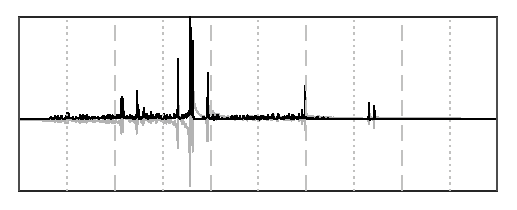
\includegraphics[width=0.95\textwidth,keepaspectratio]{images/PM_stages/pm_stages_1.eps}
    %     \caption{Original basis functions}
    %     \label{fig:PM_stages:basis functions}\vspace{0.2\baselineskip}
    % \end{subfigure}&
    % \begin{subfigure}[c]{0.315\textwidth}
    %     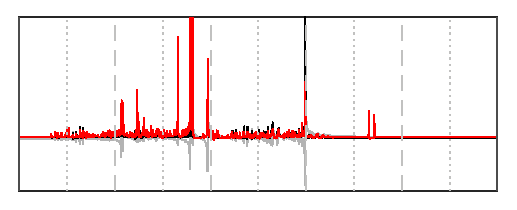
\includegraphics[width=0.95\textwidth,keepaspectratio]{images/PM_stages/pm_stages_2.eps}
    %     \caption{Modulated basis functions}
    %     \label{fig:PM_stages:modulated}\vspace{0.2\baselineskip}
    % \end{subfigure}&
    % \begin{subfigure}[c]{0.315\textwidth}
    %     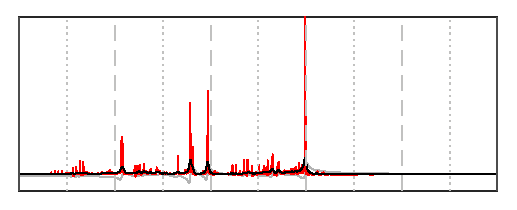
\includegraphics[width=0.95\textwidth,keepaspectratio]{images/PM_stages/pm_stages_3.eps}
    %     \caption{Voigt lineshape}
    %     \label{fig:PM_stages:B0 inhomogeneities}\vspace{0.2\baselineskip}
    % \end{subfigure}\\[25pt]
    % \begin{subfigure}[c]{0.315\textwidth}
    %     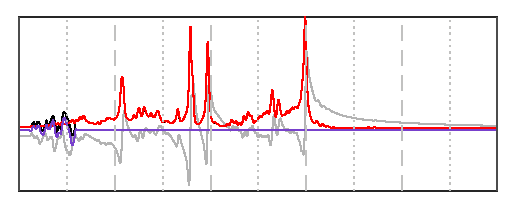
\includegraphics[width=0.95\textwidth,keepaspectratio]{images/PM_stages/pm_stages_4.eps}
    %     \caption{Residual Water}
    %     \label{fig:PM_stages:lineshape}\vspace{0.2\baselineskip}
    % \end{subfigure}&
    % \begin{subfigure}[c]{0.315\textwidth}
    %     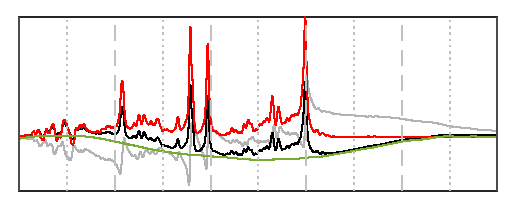
\includegraphics[width=0.95\textwidth,keepaspectratio]{images/PM_stages/pm_stages_5.eps}
    %     \caption{Baseline}
    %     \label{fig:PM_stages:phi1}\vspace{0.2\baselineskip}
    % \end{subfigure}&
    % \begin{subfigure}[c]{0.315\textwidth}
    %     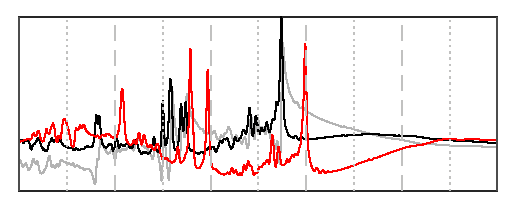
\includegraphics[width=0.95\textwidth,keepaspectratio]{images/PM_stages/pm_stages_6.eps}
    %     \caption{Frequency Shift}
    %     \label{fig:PM_stages:phi0}\vspace{0.2\baselineskip}\vspace{0.2\baselineskip}
    % \end{subfigure}\\[25pt]
    % \begin{subfigure}[c]{0.315\textwidth}
    %     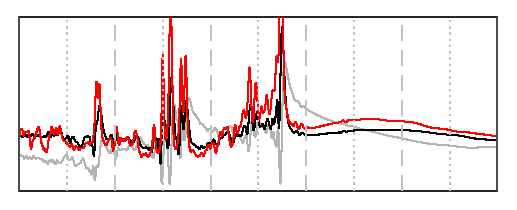
\includegraphics[width=0.95\textwidth,keepaspectratio]{images/PM_stages/pm_stages_7.eps}
    %     \caption{Eddy currents}
    %     \label{fig:PM_stages:fshift}\vspace{0.2\baselineskip}
    % \end{subfigure}&
    % \begin{subfigure}[c]{0.315\textwidth}
    %     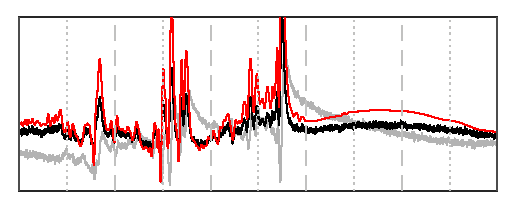
\includegraphics[width=0.95\textwidth,keepaspectratio]{images/PM_stages/pm_stages_8.eps}
    %     \caption{Noise}
    %     \label{fig:PM_stages:SNR}\vspace{0.2\baselineskip}
    % \end{subfigure}&
    % \begin{subfigure}[c]{0.315\textwidth}
    %     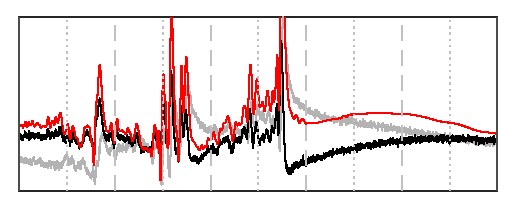
\includegraphics[width=0.95\textwidth,keepaspectratio]{images/PM_stages/pm_stages_9.eps}
    %     \caption{First-order phase}
    %     \label{fig:PM_stages:residual water}\vspace{0.2\baselineskip}
    % \end{subfigure}\\[25pt]
    % \begin{subfigure}[c]{0.315\textwidth}
    %     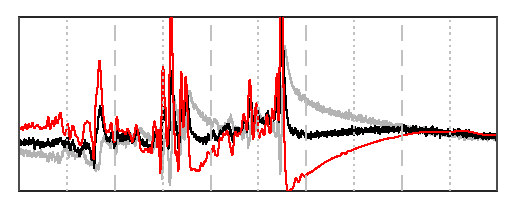
\includegraphics[width=0.95\textwidth,keepaspectratio]{images/PM_stages/pm_stages_10.eps}
    %     \vspace{0.5pt}
    %     \caption{Zero-order phase}
    %     \label{fig:PM_stages:baseline}
    % \end{subfigure}&
    % \begin{subfigure}[c]{0.315\textwidth}
    %     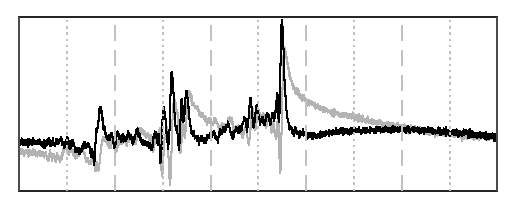
\includegraphics[width=0.95\textwidth,keepaspectratio]{images/PM_stages/pm_stages_11.eps}
    %     \vspace{0.5mm}
    %     \caption{Generated spectrum}
    %     \label{fig:PM_stages:generated spectrum}
    % \end{subfigure}&
    % \begin{subfigure}[c]{0.315\textwidth}
    %     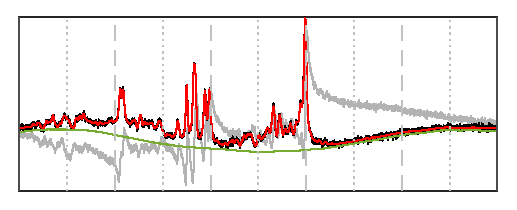
\includegraphics[width=0.95\textwidth,keepaspectratio]{images/PM_stages/pm_stages_12.eps} \smallskip
    %     \caption{Pre-processed spectrum}
    %     \label{fig:PM_stages:corrected}
    % \end{subfigure}
    % \end{tabular}
    \includegraphics[width=\textwidth,keepaspectratio]{images/compiled_figures/MRS_Sim_Figure_1_PM_stages_1.png}
    \caption{This is a step-by-step progression through the physics model. The real and imaginary components are depicted in black and gray, respectively. The red line includes only the metabolites and the offsets from the preceding steps. \ref{fig:PM_stages:generated spectrum} shows the final spectrum with all artifacts applied. \ref{fig:PM_stages:corrected} is the pre-processed spectrum with the phase and frequency shifts removed.}
    \label{fig:PM compilation}
\end{figure}


\subsubsection{Basis Functions}
MRI, and its derivatives, are spatially resolved imaging modalities. MR pixels and voxels represent 3D volumes with a spatial distribution, as shown in Fig. \ref{fig:spatial voxel}, and needs to be accounted for in simulations. The importance of spatial localization led to selecting Landheer \etal's Magnetic Resonance Spectrum Simulator (MARSS)\cite{Landheer2021} software package for simulating the default basis functions provided with this simulator. MARSS produces high-fidelity outputs by simulating 128 points in each direction, accurately capturing the spatial nature the RF pulses and slice-selective gradients. Using vendor-specific pulse sequences, MARSS can simulate individual or summed spins for a large number of common brain metabolites including macromolecules and lipids.% vendor-specific basis functions making it easy to use for new simulations. 
% The default basis functions are stored as individual spins for each metabolite allowing fine-detailed artifacts to be included. %for these metabolites can be simulated with PRESS and STEAM sequences. Custom basis functions can also be simulated with various metabolites, T1 and T2 relaxations, and specialized pulse sequences, e.g. editing sequences, (semi-)LASER, etc.
 
\begin{figure}[b]
    \centering
    % \begin{tabular}[b]{>{\centering}b{0.315\textwidth}>{\centering}b{0.315\textwidth}>{\centering}b{0.315\textwidth}}
    %     \centering
    %     \begin{subfigure}[c]{0.315\textwidth}
    %         \centering
    %         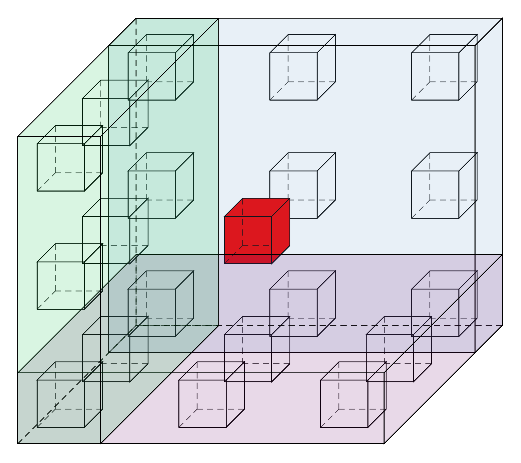
\includegraphics[width=5cm,keepaspectratio]{images/spatial_localization.eps}
    %         \caption{Intravoxel localization}
    %         \label{fig:spatial voxel}
    %     \end{subfigure} & 
    %     \begin{subfigure}[c]{0.315\textwidth}
    %         \centering
    %         \def\svgwidth{5cm}
    %         \input{images/B0_inhomogeneity_cube.eps_tex}
    %         \caption{Intravoxel spatial distribution of $B_0$ with minor distortions}
    %         \label{fig:spatial B0}
    %     \end{subfigure} &
    %     \begin{subfigure}[c]{0.315\textwidth}
    %         \centering
    %         \def\svgwidth{5cm}
    %         \input{images/B0_inhomogeneity_cube_severe_distortion.eps_tex}
    %         \caption{Spatial distribution of $B_0$ with major distortions}
    %         \label{fig:spatial B0 severe}
    %     \end{subfigure}
    % \end{tabular}
    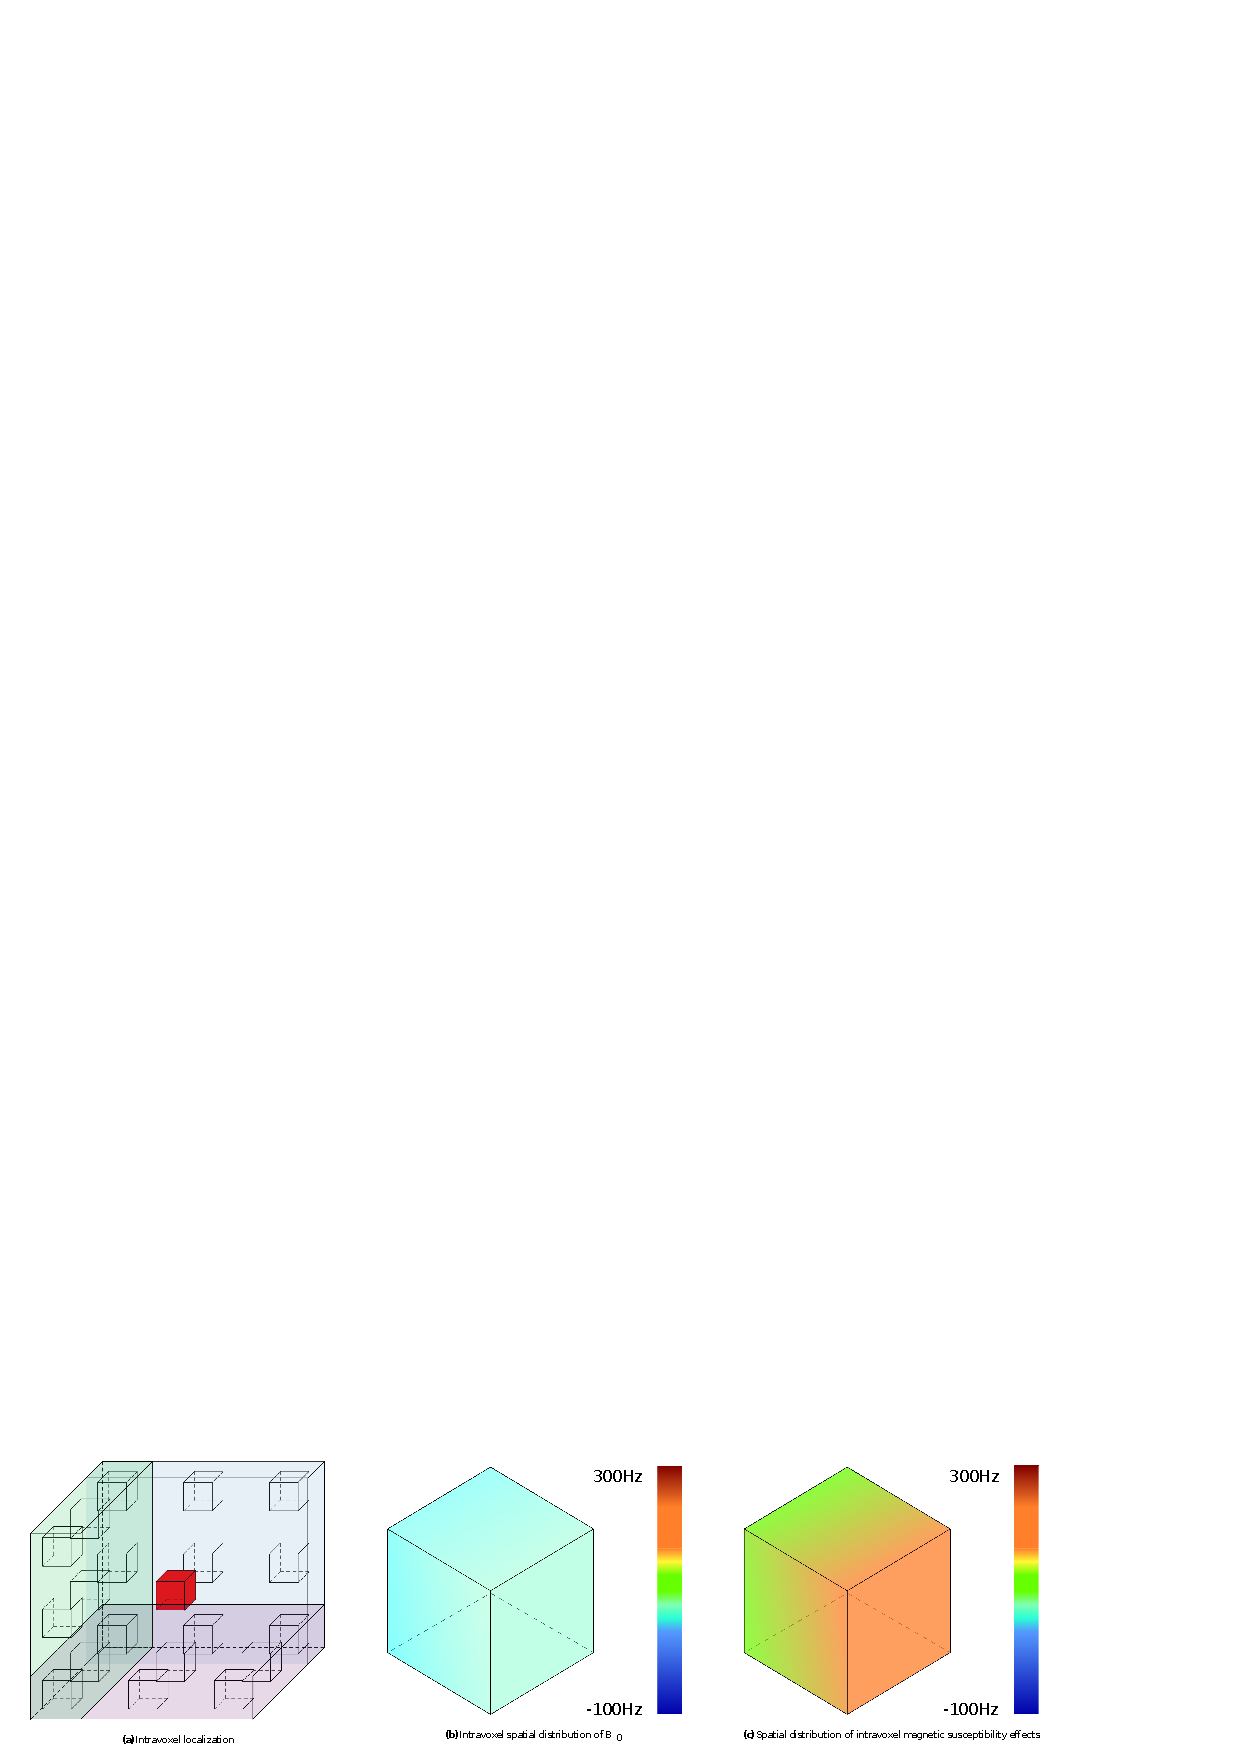
\includegraphics[width=\textwidth, keepaspectratio]{images/compiled_figures/MRS-Sim_Figure2_Spatial_localization.png}
    \caption{Voxels are often treated as singularities, meaning the entire volume is considered to be a single point like the red box in the center. Accounting for these intravoxel distributions leads to more accurate and more realistic simulations. \ref{fig:spatial voxel} highlights the spatial nature of voxels while \ref{fig:spatial B0} and \ref{fig:spatial B0 severe} show different levels of intravoxel $B_0$ inhomogeneity.}
    \label{fig:intravoxel localization}
\end{figure}

 
% \paragraph{Macromolecules and Lipids}
% Current spectral fitting methods for modeling MM and lipid signals are based on creating a group of curves that resemble clinical data but are not informed by any underlying physical phenomenon. Each fitting package contains their own set of basis functions for modeling these regions. Until this knowledge gap is filled and better simulation methods are developed, this work will use pre-generated basis functions from Osprey\cite{Oeltzschner2020}.% that were resampled to match the simulated basis functions from MARSS.
 
\subsubsection{Amplitude Modulation}
For this framework, comprehensive ranges including physiological and pathological values were adapted from the meta-analysis by Gudmundson \etal\cite{Gudmundson2023}. Near\cite{Near2021} and Larsen\cite{Larsen2021} discuss how non-trivial the choice of reference metabolite is with respect to quantification and interpretability. Therefore, the default ranges are in units of milimolar (mM) which allows any reference to be used. More specific information can be found in the MARSS user manual.
% Metabolite quantities produced during spectral fitting are of an arbitrary scale. Comparing these quantities with a standard reference puts them into context. In vivo proton scans generally use an internal reference metabolite for relative quantification. Creatine is the default metabolite because its concentration is relatively stable. As a result, concentrations maps are generally reported as ratios with respect to creatine and all amplitude values in this model are defined \textit{wrt} creatine as the default. For this framework, comprehensive ranges including physiological and pathological values were adapted from the meta-analysis by Gudmundson \etal\cite{Gudmundson2023}. 
%These ranges were then expanded to include values observed in in vivo scans from a private glioma dataset. In keeping in line with the LCModel, the expected concentrations ranges represent the scaling factors needed for spectral fitting instead of the ratios of peak integrals or peak heights.
 
\subsubsection{Lineshape Profiles}\label{subsubsec:lineshapes}
The Voigt lineshape profile is the most commonly used in spectral fitting as it most closely matches in vivo data.
% In spectral fitting, the Voigt lineshape profile is the most commonly used as it most closely matches clinical data. 
It is a combination of a Lorentzian and a Gaussian and is used in various fitting packages, such as LCModel\cite{Provencher2001}, TARQUIN\cite{Wilson2011}, jMRUI\cite{Stefan2009}, and Osprey\cite{Oeltzschner2020}. For completeness, it is also possible to specify either a purely Lorentzian or a purely Gaussian lineshape. 
Individual Lorentzian and Gaussian values can be assigned to each moiety or metabolite separately, depending on the desired level of granularity. At the most basic level, each metabolite is assigned a Lorentzian value while a single Gaussian value is applied to the set of metabolites and a second value can be applied to the macromolecules and lipids. Standard practice from the aforementioned software packages assigns a single Lorentzian value to each metabolite, instead of each moiety. However, experimental results from Wyss \etal\cite{Wyss2018} can be used, which characterized moiety-level T2 relaxation values for metabolites in three brain regions at 3T. Information for some metabolites can be supplemented by the meta-analysis from Gudmundson \etal\cite{Gudmundson2023}. As more metabolites are characterized, new information can be added to the model. A detailed table will be provided in the appendix with the current information, however a digital version that can be updated will also be maintained in the repository.
 
\subsubsection{$B_0$ Inhomogeneities}
% Lower and higher order shimming procedures homogenize the magnetic field in the target volume to different degrees. However, certain regions of the brain, such as the prefrontal cortex or deep brain structures like the thalamus or basal ganglia, are more difficult to shim and therefore suffer from large magnetic susceptibility effects, resulting in significant lineshape distortions. Fig. \ref{fig:spatial B0} shows the normal, subtle $B_0$ changes across the volume of a spectroscopy voxel while Fig. \ref{fig:spatial B0 severe} illustrates these high susceptibility effects. In such cases, spectra from these regions exhibit significant lineshape distortions which cannot be adequately characterized using idealized lineshape profiles. Fig. \ref{fig:B0 effects} shows the result of high susceptibility effects on lineshapes.

% \begin{figure}
    \centering
    \begin{subfigure}{0.32\textwidth}
        \centering
        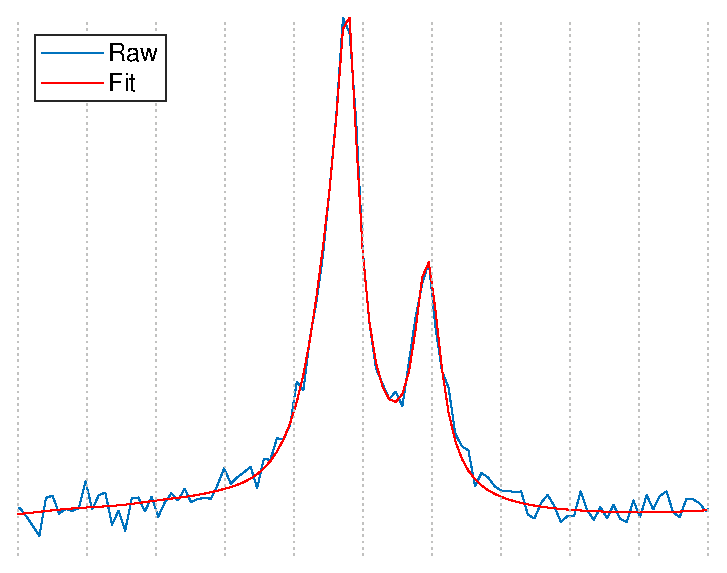
\includegraphics[width=0.95\textwidth,keepaspectratio]{images/b0_peaks/no_B0.eps}
        \caption{Spectral peaks without $B_0$ inhomogeneities ($\mu = 0$Hz)}
        \label{subfig:without B0}        
    \end{subfigure}
    \begin{subfigure}{0.32\textwidth}
        \centering
        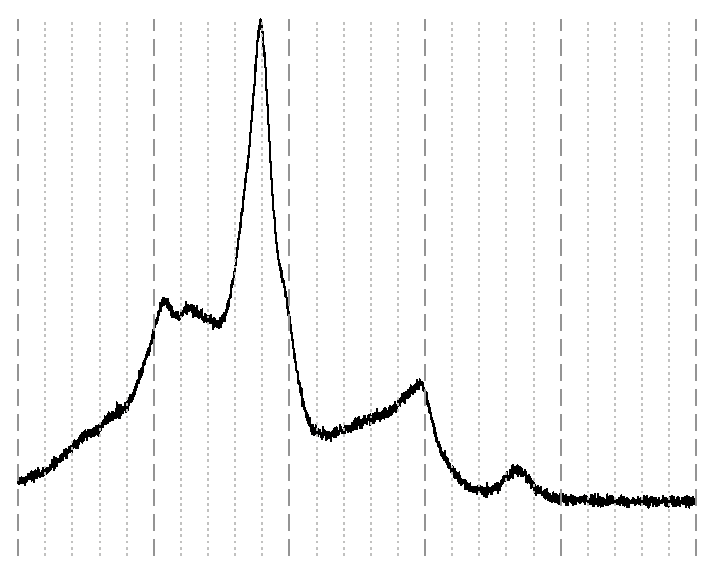
\includegraphics[width=0.95\textwidth,keepaspectratio]{images/b0_peaks/some_B0.eps}
        \caption{Spectral peaks with moderate $B_0$ inhomogeneities ($\mu = 75$Hz)}
        \label{subfig:some B0}        
    \end{subfigure}
    \begin{subfigure}{0.32\textwidth}
        \centering
        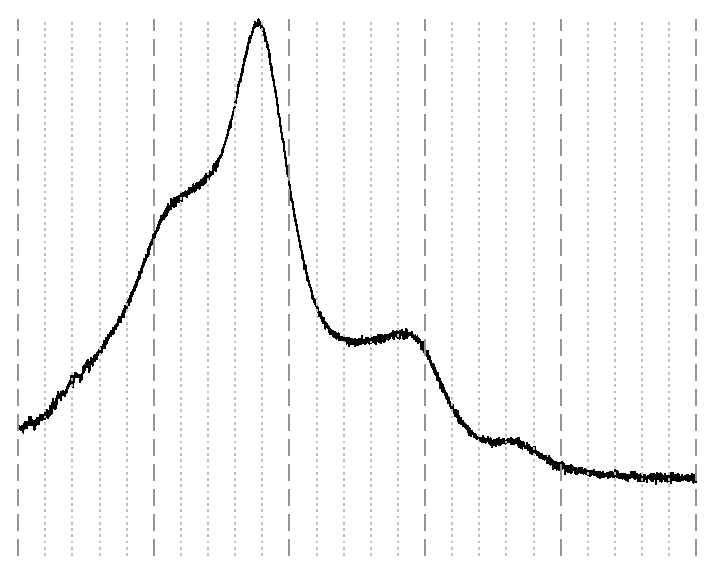
\includegraphics[width=0.95\textwidth,keepaspectratio]{images/b0_peaks/with_B0.eps}
        \caption{Spectral peaks with severe $B_0$ inhomogeneities ($\mu = 175$Hz)}
        \label{subfig:with B0}        
    \end{subfigure}
    \caption{These samples show the effects that can be modeled using the 3D $B_0$ field simulator. In \ref{subfig:without B0}, the spectral peaks have a purely Lorentzian lineshape. In \ref{subfig:some B0}, the lineshape is now Voigtian because the Gaussian term has been added back by the 3D $B_0$ field simulator. In \ref{subfig:with B0}, severe heterogeneities are modeled which produce extremely broad line widths. All three plots use the same x- and y-axes. The observed offsets are caused by the line broadening.}
    \label{fig:B0 effects}
\end{figure}


Small $B_0$ inhomoegeneities are, in general, sufficiently modeled by the Gaussian term of the Voigt lineshape. However, to simulate more severe distortions from large inhomogeneities, a $B_0$ field volume needs to be modeled and applied to the basis functions. Fig. \ref{fig:intravoxel localization} illustrates the difference between small and severe $B_0$ inhomogeneities. Fig. \ref{fig:spatial B0} shows the normal, subtle $B_0$ changes across the volume of a spectroscopy voxel while Fig. \ref{fig:spatial B0 severe} illustrates these high susceptibility effects. In such cases, spectra from these regions exhibit significant lineshape distortions which cannot be adequately characterized using idealized lineshape profiles. Fig. \ref{fig:B0 effects} shows the result of high susceptibility effects on lineshapes.

\begin{figure}
    \centering
    \begin{subfigure}{0.32\textwidth}
        \centering
        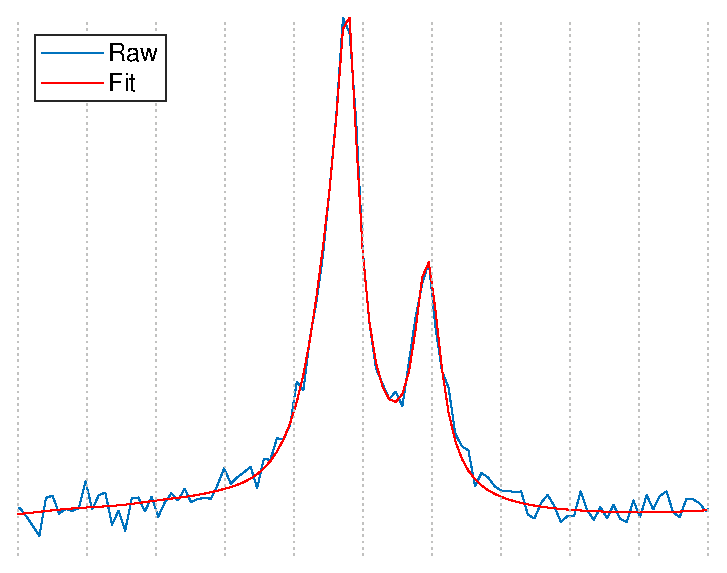
\includegraphics[width=0.95\textwidth,keepaspectratio]{images/b0_peaks/no_B0.eps}
        \caption{Spectral peaks without $B_0$ inhomogeneities ($\mu = 0$Hz)}
        \label{subfig:without B0}        
    \end{subfigure}
    \begin{subfigure}{0.32\textwidth}
        \centering
        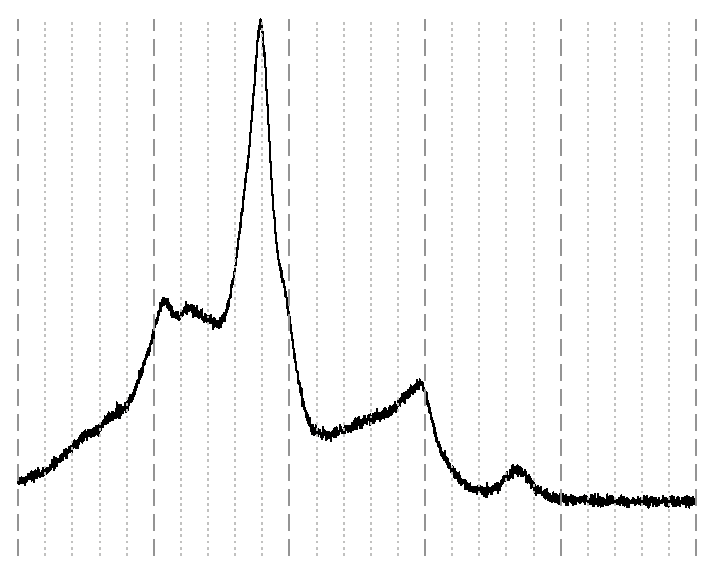
\includegraphics[width=0.95\textwidth,keepaspectratio]{images/b0_peaks/some_B0.eps}
        \caption{Spectral peaks with moderate $B_0$ inhomogeneities ($\mu = 75$Hz)}
        \label{subfig:some B0}        
    \end{subfigure}
    \begin{subfigure}{0.32\textwidth}
        \centering
        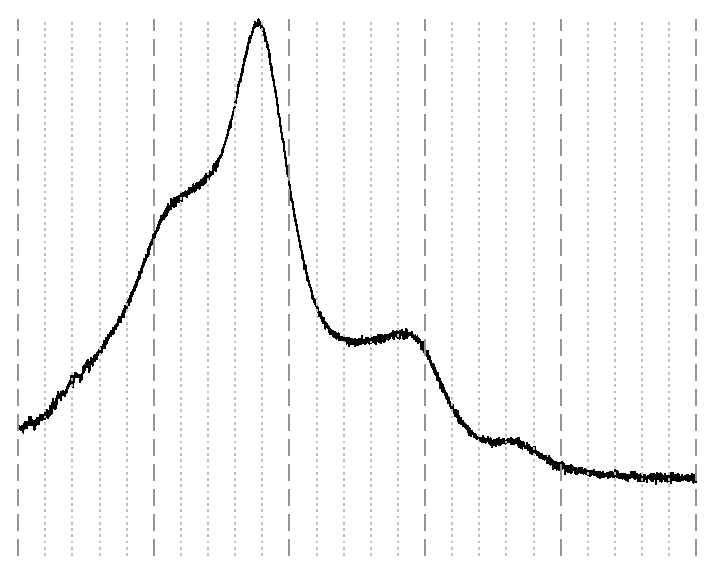
\includegraphics[width=0.95\textwidth,keepaspectratio]{images/b0_peaks/with_B0.eps}
        \caption{Spectral peaks with severe $B_0$ inhomogeneities ($\mu = 175$Hz)}
        \label{subfig:with B0}        
    \end{subfigure}
    \caption{These samples show the effects that can be modeled using the 3D $B_0$ field simulator. In \ref{subfig:without B0}, the spectral peaks have a purely Lorentzian lineshape. In \ref{subfig:some B0}, the lineshape is now Voigtian because the Gaussian term has been added back by the 3D $B_0$ field simulator. In \ref{subfig:with B0}, severe heterogeneities are modeled which produce extremely broad line widths. All three plots use the same x- and y-axes. The observed offsets are caused by the line broadening.}
    \label{fig:B0 effects}
\end{figure}


In general, this approach mirrors Li \etal\cite{Li2015} in which the basis functions are modulated by the $B_0$ field map, but in the implmenetation the $B_0$ field map is simulated rather than acquired. As with MARSS, Li \etal\ suggests using multiple points in each direction instead of a single value per voxel. The exact number of points used in each direction is described by the size of the spectroscopy voxel divided by the size of an anatomical imaging voxel. %The default values assume sizes of 10cm$^3$ and 0.5cm$^3$ respectively, which results in $20^3$ simulation points. 
% However, a
Any cuboidal shape, rectangular or otherwise, can be modeled. The $B_0$ field is defined by four variables: $\pm dx$, $\pm dy$, $\pm dz$, and $\mu$. $dx, dy,$ and $dz$ describe half of the change in $B_0$ in their respective axis from the voxel's center and $\mu$ is the mean of the entire voxel. A linear $B_0$ gradient is assumed, but other shapes can be implemented. The first section in the supplement provides a more detailed explanation for how the $B_0$ is simulated.

% Lower and higher order shimming procedures homogenize the magnetic field in the target volume to different degrees. However, certain regions of the brain, such as the prefrontal cortex or deep brain structures like the thalamus or basal ganglia, are more difficult to shim and therefore suffer from large magnetic susceptibility effects, resulting in significant lineshape distortions. Fig. \ref{fig:spatial B0} shows the normal, subtle $B_0$ changes across the volume of a spectroscopy voxel while Fig. \ref{fig:spatial B0 severe} illustrates these high susceptibility effects. In such cases, spectra from these regions exhibit significant lineshape distortions which cannot be adequately characterized using idealized lineshape profiles. Fig. \ref{fig:B0 effects} shows the result of high susceptibility effects on lineshapes.

% \begin{figure}
    \centering
    \begin{subfigure}{0.32\textwidth}
        \centering
        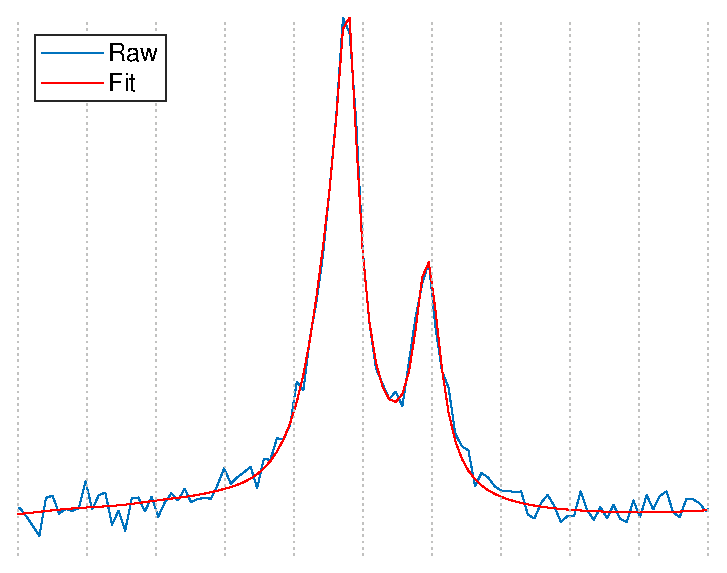
\includegraphics[width=0.95\textwidth,keepaspectratio]{images/b0_peaks/no_B0.eps}
        \caption{Spectral peaks without $B_0$ inhomogeneities ($\mu = 0$Hz)}
        \label{subfig:without B0}        
    \end{subfigure}
    \begin{subfigure}{0.32\textwidth}
        \centering
        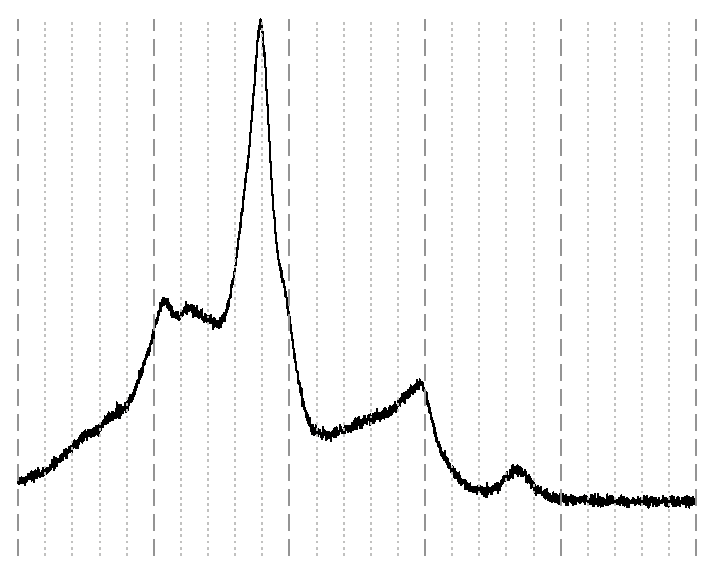
\includegraphics[width=0.95\textwidth,keepaspectratio]{images/b0_peaks/some_B0.eps}
        \caption{Spectral peaks with moderate $B_0$ inhomogeneities ($\mu = 75$Hz)}
        \label{subfig:some B0}        
    \end{subfigure}
    \begin{subfigure}{0.32\textwidth}
        \centering
        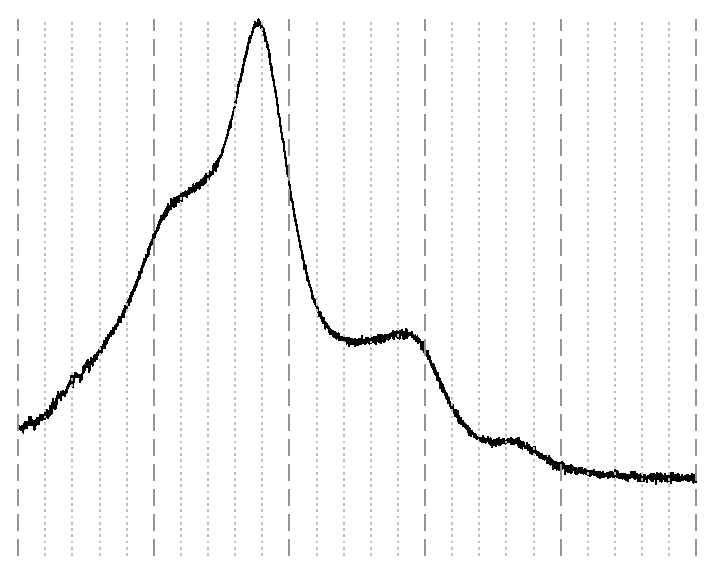
\includegraphics[width=0.95\textwidth,keepaspectratio]{images/b0_peaks/with_B0.eps}
        \caption{Spectral peaks with severe $B_0$ inhomogeneities ($\mu = 175$Hz)}
        \label{subfig:with B0}        
    \end{subfigure}
    \caption{These samples show the effects that can be modeled using the 3D $B_0$ field simulator. In \ref{subfig:without B0}, the spectral peaks have a purely Lorentzian lineshape. In \ref{subfig:some B0}, the lineshape is now Voigtian because the Gaussian term has been added back by the 3D $B_0$ field simulator. In \ref{subfig:with B0}, severe heterogeneities are modeled which produce extremely broad line widths. All three plots use the same x- and y-axes. The observed offsets are caused by the line broadening.}
    \label{fig:B0 effects}
\end{figure}


% Small $B_0$ inhomoegeneities are, in general, sufficiently modeled by the Gaussian term of the Voigt lineshape. However, to simulate more severe distortions, a $B_0$ field volume needs to be modeled and applied to the basis functions. In general, this approach mirrors Li \etal\cite{Li2015}, but the $B_0$ field map is simulated rather than acquired. As with MARSS, Li \etal\ suggests using multiple points in each direction instead of a single value per voxel. The exact number of points used in each direction is described by the size of the spectroscopy voxel divided by the size of an anatomical imaging voxel. The default values assume sizes of 10cm$^3$ and 0.5cm$^3$ respectively, which results in $20^3$ simulation points. However, any cuboidal shape, rectangular or otherwise, can be modeled. The $B_0$ field is defined by four variables, all of which are mean offsets: $\pm dx$, $\pm dy$, $\pm dz$, and $\mu$. $dx, dy,$ and $dz$ describe half of the change in $B_0$ in their respective direction from the voxel's center and $\mu$ is the mean of the entire voxel. 

\begin{figure}[b!]
    \centering
    \begin{tabular}[l]{cc}
    \begin{subfigure}{0.49\textwidth}
        \centering
        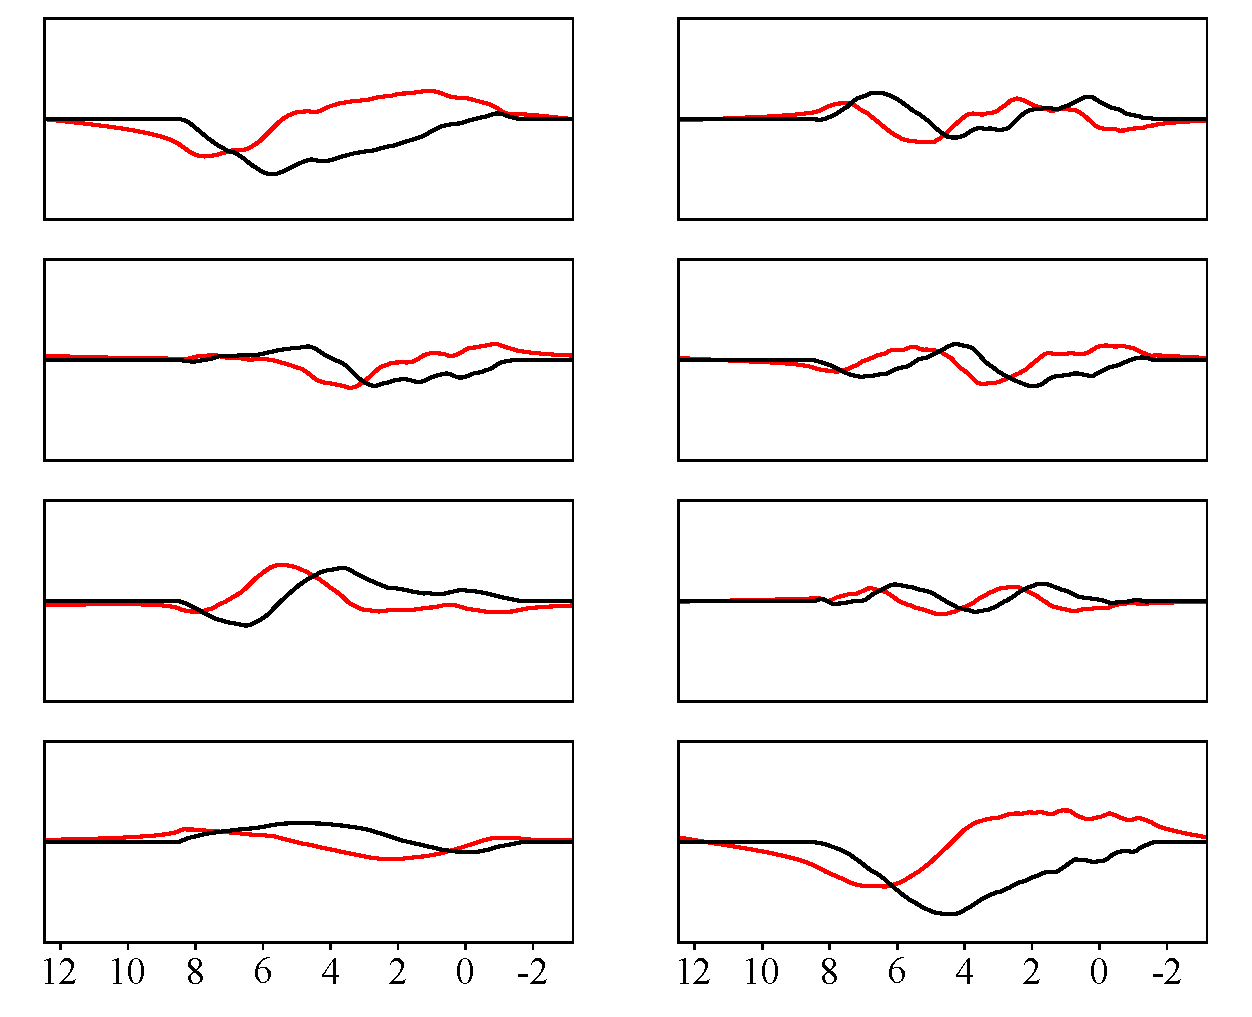
\includegraphics[width=0.95\textwidth,keepaspectratio]{images/random_walks/baseline_walks_edited.eps}
        \caption{Simulated baselines}
        \label{fig:baseline_region}
    \end{subfigure} &
    
    \begin{subfigure}{0.49\textwidth}
        \centering
        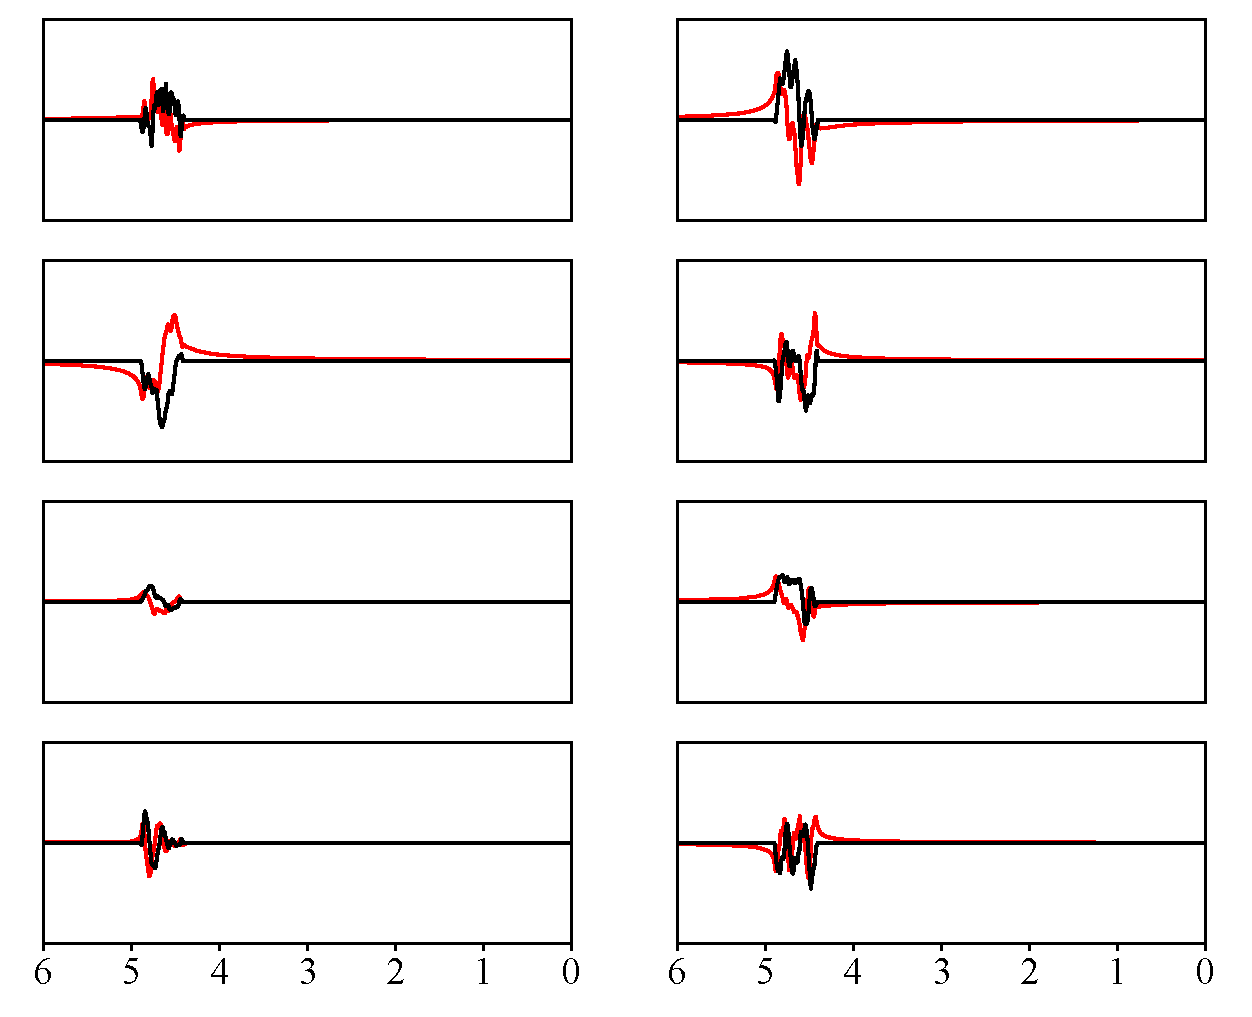
\includegraphics[width=0.95\textwidth,keepaspectratio]{images/random_walks/reswater_walks_edited.eps}
        \caption{Simulated residual water}
        \label{fig:reswater_region}
    \end{subfigure}
    \end{tabular}
    \caption{Simulated  samples of spectral baselines and residual water regions using the pseudo-random bounded walk generator. The blue lines are the raw simulations. The red lines are the smoothed versions that are then returned and applied to the simulated spectra.}
    \label{fig:random walk generator}
\end{figure}

\begin{algorithm}[t!]
\caption{Smoothed Bounded Pseudo-Random Walk} \label{alg:smoothed bounded pseudo-random walk}
\begin{algorithmic}[1]
\Require $start$: ppm start value, $end$: ppm end value, $std$: standard deviation of the random noise, $lower\_bound$: lower bound of the walk, $upper\_bound$: upper bound of the walk, $length$: length of the walk
% \Ensure $rand\_walk$: bounded pseudo-random walk
\end{algorithmic}

\textbf{Function} SmoothedBoundedPseudoRandomWalk($start, end, std, lower\_bound, upper\_bound, length, window\_size$)
% \Function{BoundedPseudoRandomWalk}{$start, end, std, lower\_bound, upper\_bound, length$}
\begin{algorithmic}[1]
\State $bounds = upper\_bound - lower\_bound$
\Statex Generate raw random walk
\State $rand = \text{generate\_random\_array}(size=length, std=std)$
\State $rand = \text{cumsum}(rand, dim=-1)$

\Statex Calculate the trend line
\State $rand\_trend\_lines = \text{generate\_trend\_array}(start, end, length)$

\Statex Calculate the difference between the random steps and the trend line
\State $rand\_deltas = rand - rand\_trend\_lines$
\Statex Normalize the delta array
\State $delta\_range = bounds \div (rand\_deltas.max() - rand\_deltas.min())$
\State $rand\_deltas = rand\_deltas * delta\_range$

\Statex Adjust delta array if it exceeds \textit{bounds}
\State $rand\_deltas = conditional\_adjustment(rand\_deltas)$
\Statex Calculate the final random walk
\State $random\_walk = trend\_lines + rand\_deltas$

\Statex Smooth using a uniform smoothing kernel
% \State $kernel\_size $
\State $random\_walk = \text{average\_smoothing}(random\_walk, kernel\_size=window\_size * length)$

\Statex \Return $random\_walk$ %trend\_lines + rand_deltas$
% \EndFunction
\end{algorithmic}
\end{algorithm}

 
\subsubsection{Baseline and Residual Water}


Currently, the underlying physical phenomena that induce spectral baseline offsets are poorly understood. In fact, there is no physics-based model for simulating these offsets. Similarly, the residual water region is also poorly characterized. Therefore, a naive random model can be used in conjunction with observed constraints to approximate what is expected in vivo. This work proposes a smoothed, pseudo-random, bounded walk generator for both the broad spectral baseline and the more irregular residual water region. The approach is elaborated on in Algorithm \ref{alg:smoothed bounded pseudo-random walk}. Customizable profiles were developed for each artifact to more closely approximate what is expected in vivo. Immense variety of outputs can be achieved by randomly sampling the parameters from distributions instead of using fixed values. Once simulated, they are resampled to match the ppm range of acquired data and the order of magnitude is matched to the spectra. The Hilbert transform is then used to generate the corresponding complex component before being added to the FID. As shown in Fig. \ref{fig:random walk generator}, this generator produces very different outputs depending on the specified configurations. Fig. \ref{fig:baseline_region} shows very broad, smooth lines while Fig. \ref{fig:reswater_region} shows highly irregular lines that closely resemble residual water regions. All outputs are then scaled to modulate the impact on the final spectra. A more detailed exploration of this algorithm and the effects of each parameter are presented in the supplement for baseline and residual water simulations.

% \begin{algorithm}[t!]
\caption{Smoothed Bounded Pseudo-Random Walk} \label{alg:smoothed bounded pseudo-random walk}
\begin{algorithmic}[1]
\Require $start$: ppm start value, $end$: ppm end value, $std$: standard deviation of the random noise, $lower\_bound$: lower bound of the walk, $upper\_bound$: upper bound of the walk, $length$: length of the walk
% \Ensure $rand\_walk$: bounded pseudo-random walk
\end{algorithmic}

\textbf{Function} SmoothedBoundedPseudoRandomWalk($start, end, std, lower\_bound, upper\_bound, length, window\_size$)
% \Function{BoundedPseudoRandomWalk}{$start, end, std, lower\_bound, upper\_bound, length$}
\begin{algorithmic}[1]
\State $bounds = upper\_bound - lower\_bound$
\Statex Generate raw random walk
\State $rand = \text{generate\_random\_array}(size=length, std=std)$
\State $rand = \text{cumsum}(rand, dim=-1)$

\Statex Calculate the trend line
\State $rand\_trend\_lines = \text{generate\_trend\_array}(start, end, length)$

\Statex Calculate the difference between the random steps and the trend line
\State $rand\_deltas = rand - rand\_trend\_lines$
\Statex Normalize the delta array
\State $delta\_range = bounds \div (rand\_deltas.max() - rand\_deltas.min())$
\State $rand\_deltas = rand\_deltas * delta\_range$

\Statex Adjust delta array if it exceeds \textit{bounds}
\State $rand\_deltas = conditional\_adjustment(rand\_deltas)$
\Statex Calculate the final random walk
\State $random\_walk = trend\_lines + rand\_deltas$

\Statex Smooth using a uniform smoothing kernel
% \State $kernel\_size $
\State $random\_walk = \text{average\_smoothing}(random\_walk, kernel\_size=window\_size * length)$

\Statex \Return $random\_walk$ %trend\_lines + rand_deltas$
% \EndFunction
\end{algorithmic}
\end{algorithm}

 
\subsubsection{Noise}
The noise in this model assumes a Gaussian distribution. The input SNR is first converted from decibels to a linear SNR. Then the standard deviation for this distribution is calculated using the maximum height of a metabolite of choice in the real spectrum and the desired SNR. The real and imaginary components of the noise can be correlated using the Hilbert transform. If they are assumed to be uncorrelated, then separate noise vectors are sampled for each component. 

\subsubsection{Phase Offsets}
% There are two types of phase offsets encountered in MRS: zero-order and first-order. FIDs and spectra are complex data type consisting of real and imaginary components. A $0^{\circ}$ zero-order phase offset results in absorption and dispersion spectra in these components, respectively. An absorption spectrum exhibits peaks with idealized lineshapes that are purely positive or purely negative, while dispersion spectra exhibit peaks that are both positive and negative. As shown in Fig. \ref{fig:phase effects}, non-zero degree offsets result in a mixture of absorption and dispersion spectra.
\paragraph{Zero-Order Phase}
FIDs and spectra are complex data type consisting of real and imaginary components. A $0^{\circ}$ zero-order phase offset results in absorption and dispersion spectra in these components, respectively. An absorption spectrum exhibits peaks with idealized lineshapes that are purely positive or purely negative, while dispersion spectra exhibit peaks that are both positive and negative. As shown in Fig. \ref{fig:phase effects}, non-zero degree offsets result in a mixture of absorption and dispersion spectra. %In absorption mode, spectral peaks directly reflect the number of hydrogens of that species and the concentration of that molecule. This relationship means that the phase has a direct impact on metabolite quantification. 
 
\paragraph{First-Order Phase}
First-order phase, i.e. linear phase, is a frequency-dependent linear offset that emanates from a reference point, i.e. the center frequency, which is typically the water peak at 4.65ppm. %but can be modified when necessary. 
A linear phase offset creates asymmetrical line shapes that grow larger as one moves away from the reference point. This is illustrated in Fig. \ref{fig:phase effects} by comparing \ref{subfig:no phase} and \ref{subfig:first order phase}. %It is specified as degrees per ppm. 

\begin{figure}
    \centering
    \begin{subfigure}{0.32\textwidth}
        \centering
        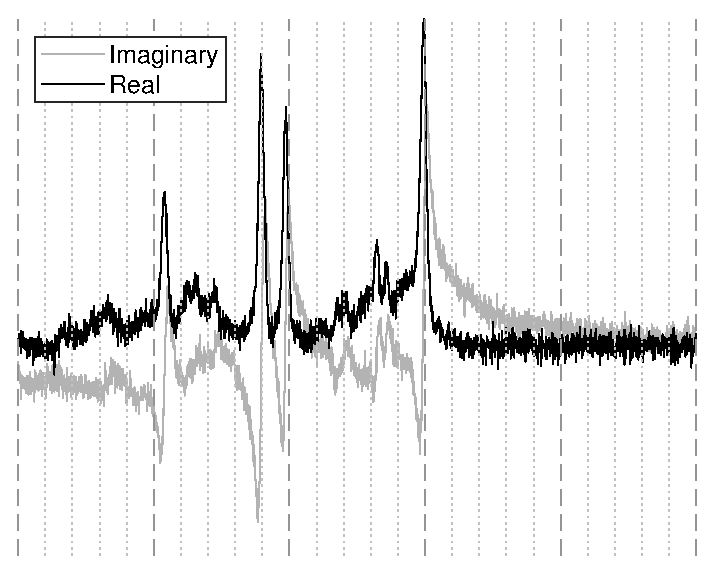
\includegraphics[width=0.95\textwidth,keepaspectratio]{images/phase/no_phase.eps}
        \caption{Spectrum with no phase offsets}
        \label{subfig:no phase}        
    \end{subfigure}
    \begin{subfigure}{0.32\textwidth}
        \centering
        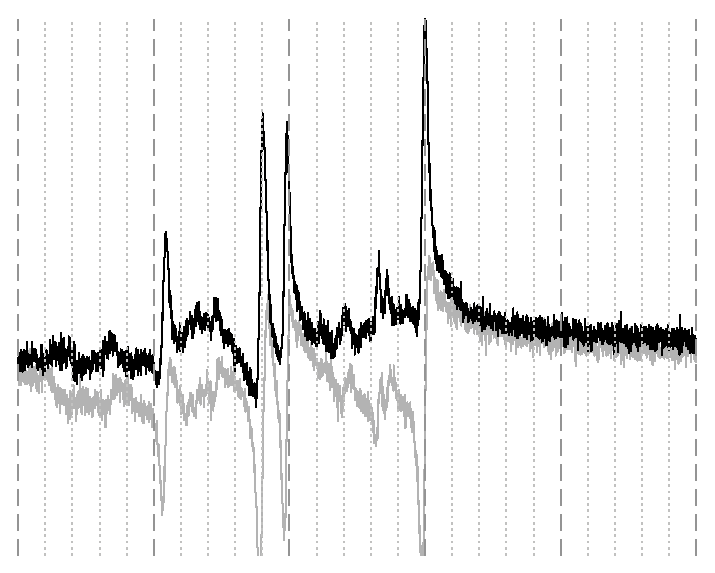
\includegraphics[width=0.95\textwidth,keepaspectratio]{images/phase/zero-order.eps}
        \caption{Spectrum with zero-order phase offset ($\phi_0 = 45^{\circ}$)}
        \label{subfig:zero order phase}        
    \end{subfigure}
    \begin{subfigure}{0.32\textwidth}
        \centering
        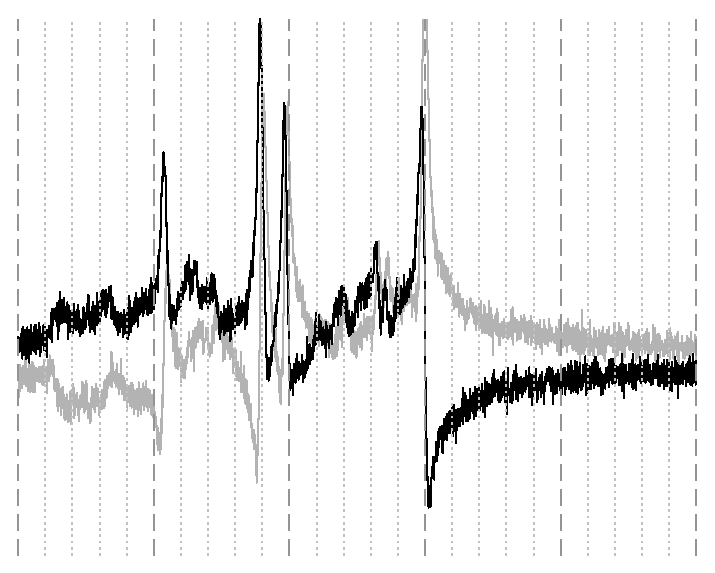
\includegraphics[width=0.95\textwidth,keepaspectratio]{images/phase/first-order.eps}
        \caption{Spectrum with first-order phase offset ($\phi_1 = 20^{\circ}$)}
        \label{subfig:first order phase}        
    \end{subfigure}
    \caption{These samples show how identical spectra are affected by zero- and first-order phase offsets. In \ref{subfig:no phase}, the real component (black) is in absorption mode exhibiting narrow line widths and is fully positive. In \ref{subfig:zero order phase}, a zero-order phase offset is applied. As the spectrum shifts from absorption to dispersion mode, the peaks uniformly lose their symmetry and negative values from the imaginary component are transferred to the real component. In \ref{subfig:first order phase}, a first-order phase shift is applied. This is evident because the asymmetry increases across the spectrum and emanates from the water peak.}
    \label{fig:phase effects}
\end{figure}
 
\subsubsection{Frequency Shifts}
% Frequency shifts observed in a spectrum result from complex interactions with a variety of factors. 
During data acquisition, the FID experiences a global frequency shift. However, some functional groups 
%individual moieties from metabolites and nuisance signals from macromolecules, lipids, and fats such as diglycerides and triglycerides, 
can experience individual frequency shifts which are attributed to effects such as temperature and pH. Similar to Sec. \ref{subsubsec:lineshapes}, the bare minimum requires separate global frequency shifts for the metabolites and nuisance signals. However, this model also allows each basis function to have an independent frequency shift in addition to the global shift which is in line with common spectral fitting protocols. For more in vivo-like, realistic spectra, values can be used from the work by Wermter \etal\cite{Wermter2017} which characterized the temperature-induced frequency shift of several brain metabolite moieties with temperature sensitivity. As more metabolites are characterized for their temperature- and pH-sensitivities, this information can be added to simulate more realistic spectra. Currently available data will be included in the table in the appendix.
 
\subsubsection{Eddy Currents}
% Eddy currents are common artifacts in MRI acquisitions that are induced by changes in the magnetic field, typically caused by the imaging gradients and present as time-dependent resonant frequency shifts. 
Eddy current correction techniques, such as the Klose\cite{Klose1990}, tend to be non-parameterized, making it difficult to model the exact effect of each approach. Near \etal\ in FID-A\cite{Simpson2017}, however, provide a parameterized equation for simulating first-order eddy currents. These artifacts are applied as a function of amplitude, $A$, time constant, $tc$, and time, $t$. The time constant must be short enough that it occurs entirely within the recorded echo, otherwise it will appear as a simple, global frequency shift. The effects of eddy currents can be seen in Fig. \ref{fig:eddy currents}.

\begin{figure}
    \centering
    % \begin{subfigure}{0.32\textwidth}
    %     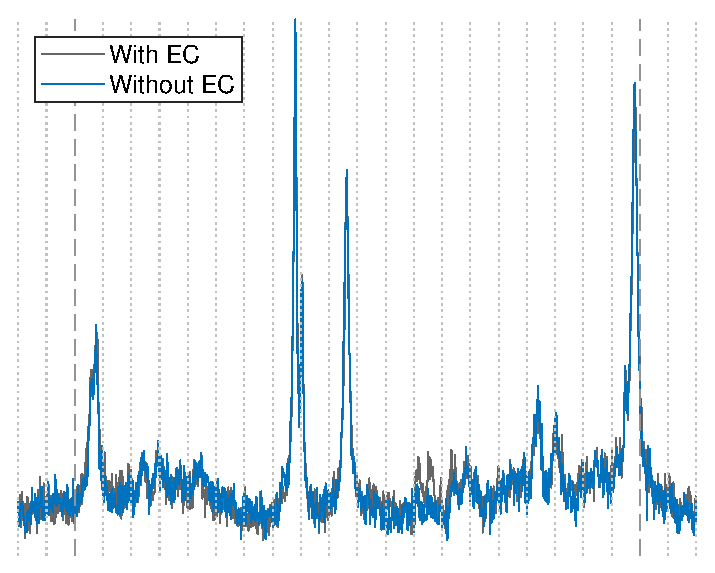
\includegraphics[width=0.95\textwidth, keepaspectratio]{images/eddy/ec=1.eps}
    %     \caption{Eddy current amplitude = 1.0}
    %     \label{subfig:ec=1}        
    % \end{subfigure}
    % \begin{subfigure}{0.32\textwidth}
    %     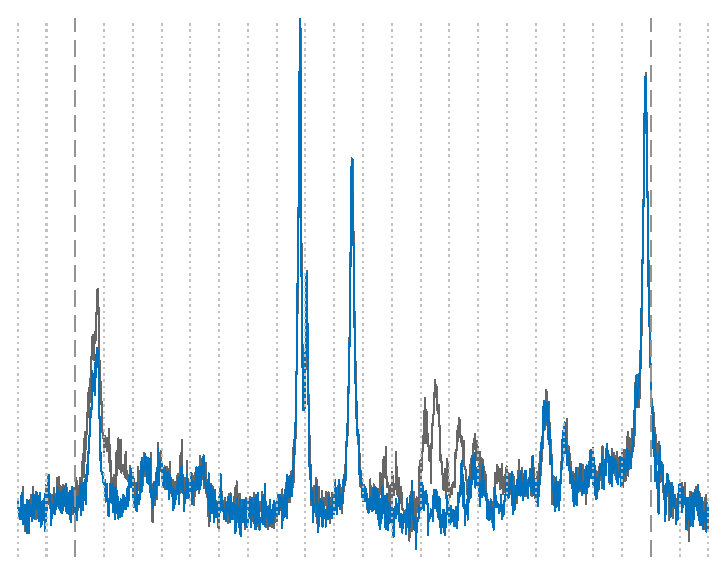
\includegraphics[width=0.95\textwidth, keepaspectratio]{images/eddy/ec=3.eps}
    %     \caption{Eddy current amplitude = 3.0}
    %     \label{subfig:ec=3}        
    % \end{subfigure}
    % \begin{subfigure}{0.32\textwidth}
    %     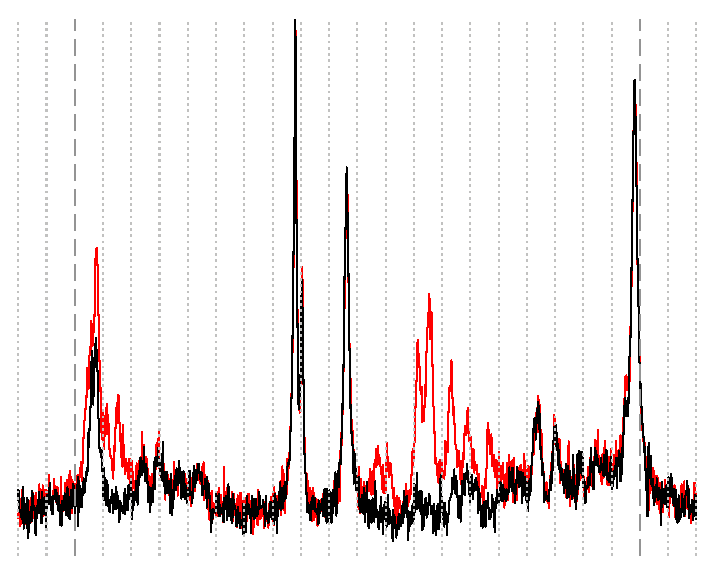
\includegraphics[width=0.95\textwidth, keepaspectratio]{images/eddy/ec=5.eps}
    %     \caption{Eddy current amplitude = 5.0}
    %     \label{subfig:ec=5}        
    % \end{subfigure}
    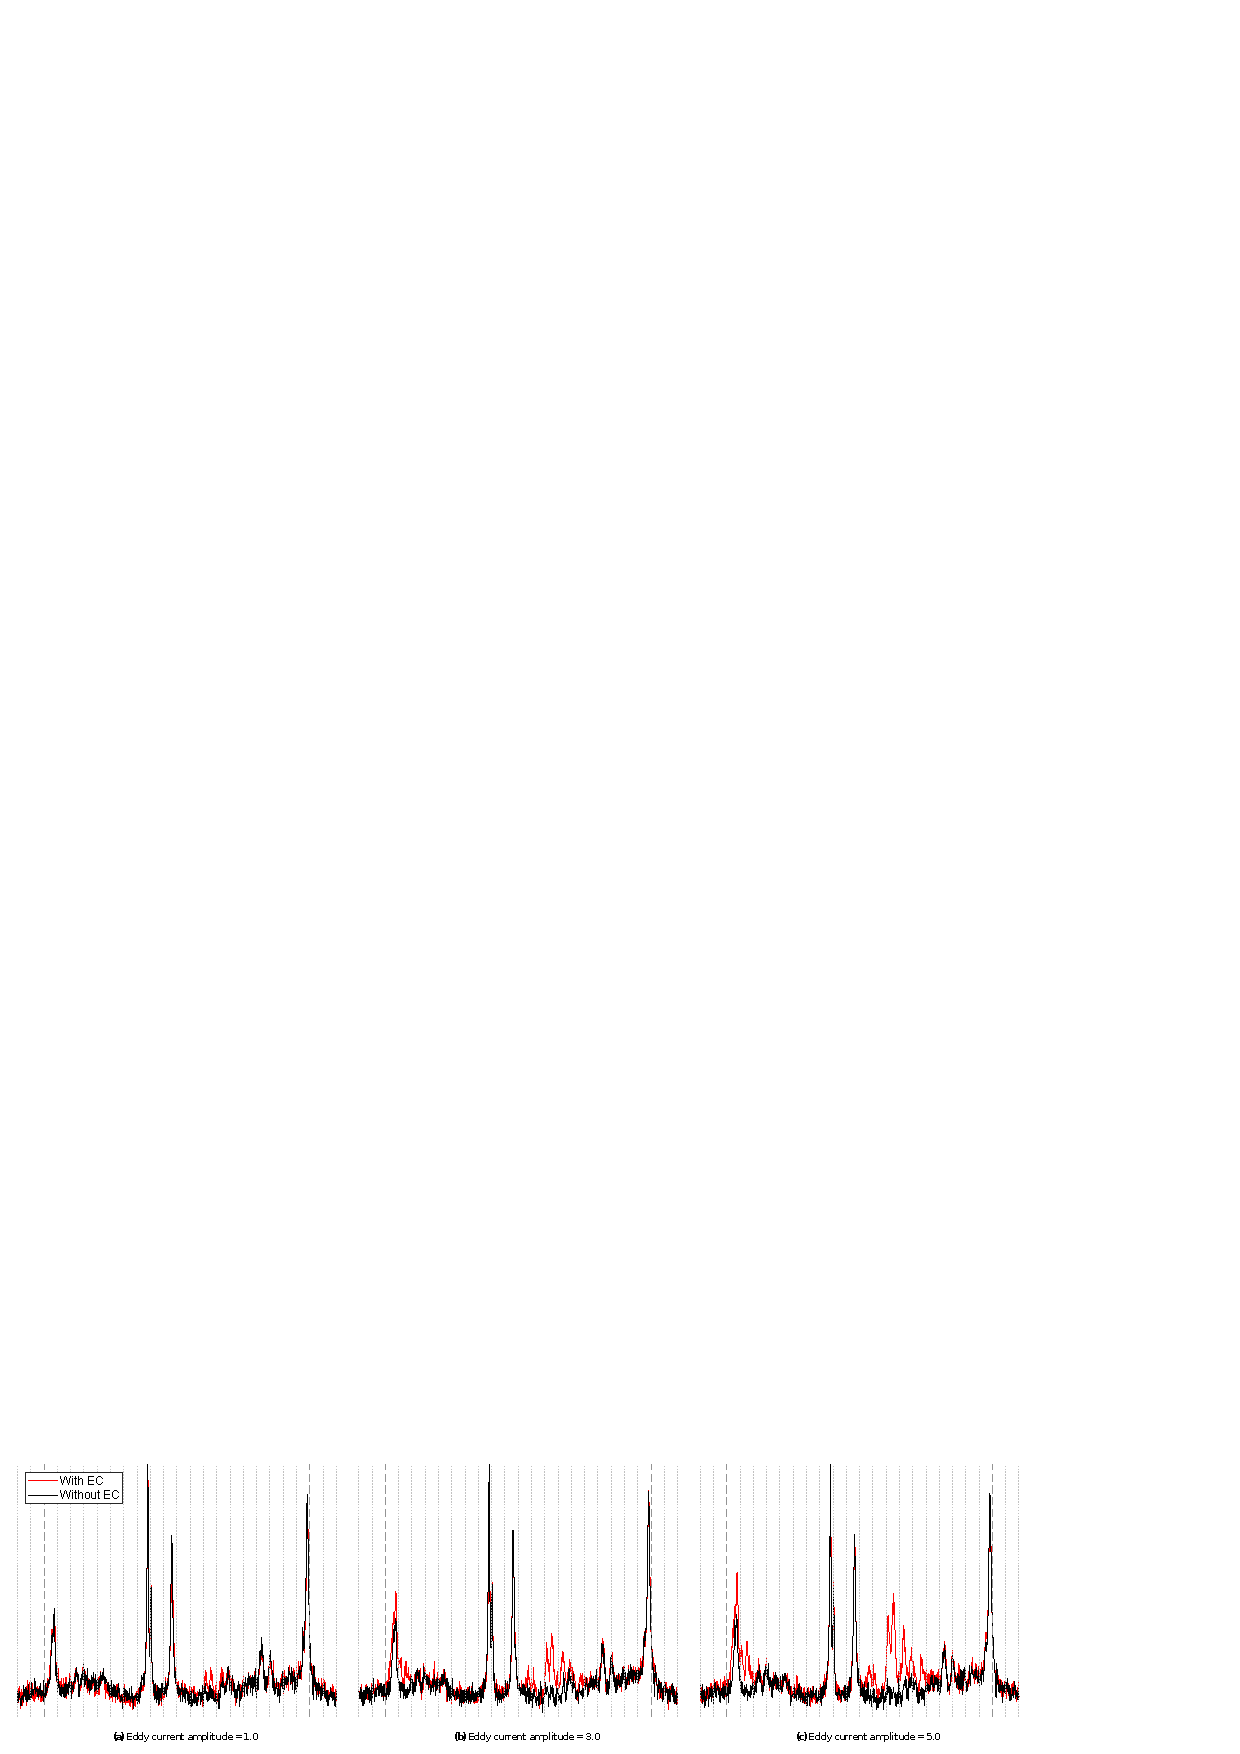
\includegraphics[width=\textwidth,keepaspectratio]{images/compiled_figures/MRS-Sim_Figure6_ eddy_current_effects.png}
    \caption{These 3 samples show the effect of eddy currents on MRS spectra to various degrees. The strength of the eddy currents increases from \ref{subfig:ec=1} to \ref{subfig:ec=5}. If the time constant, $tc$, is set too long, the eddy current artifact will appear as a global frequency shift. In these examples, it can be seen that only some frequencies are affected.}
    \label{fig:eddy currents}
\end{figure}


\subsubsection{Multi-Coil Transients}
When simulating transients, additional considerations need to be included. 
During acquisition, transients 
% A transient copy is made for each coil in the simulated scenario. These transients will 
experience additional artifacts including zero-order phase and frequency drifts, scaling due to coil sensitivity, and decreased SNR values. Each of these are included in the proposed framework. To allow for maximum variation in the simulations, each parameter can be sampled from distributions and is discussed below.

\paragraph{Noise} Averaging multi-coil acquisitions leads to an SNR improvement of the final spectrum by a factor of the square root of the number of non-zero weighted transients. To vary the SNR among the transients, this model scales the target linear SNR according to the number of coils and then samples scaling factors from a narrow normal distribution to maintain the mean target SNR. 

\paragraph{Frequency Drift and Phase Drift}
Frequency drifts and phase drifts are phenomena observed in multi-coil acquisitions in which each coil transient has an independent offset. %The lower SNR values of the transients make it harder to accurately correct these inter-transient variations. Therefore, drifts are typically minimized between the transients, called alignment. Proper alignment will preserve the underlying spectral features once the transients are combined.
These offsets and alignments are shown in Fig. \ref{fig:simulated transients}.

\begin{figure}[t]
    \centering
    \begin{subfigure}{0.32\textwidth}
        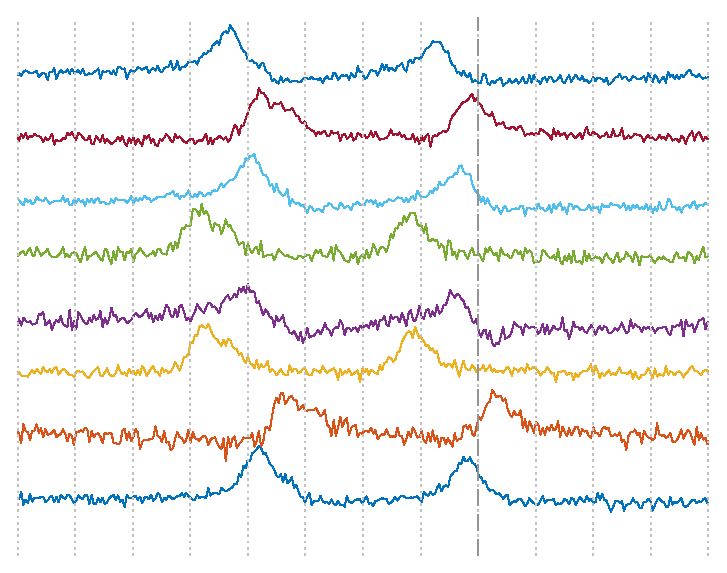
\includegraphics[width=0.95\textwidth, keepaspectratio]{images/samples_transients/8coil_w_phase_w_fshift_cropped.eps}
        \caption{Raw spectral transients}
        \label{subfig:raw transients}        
    \end{subfigure}
    \begin{subfigure}{0.32\textwidth}
        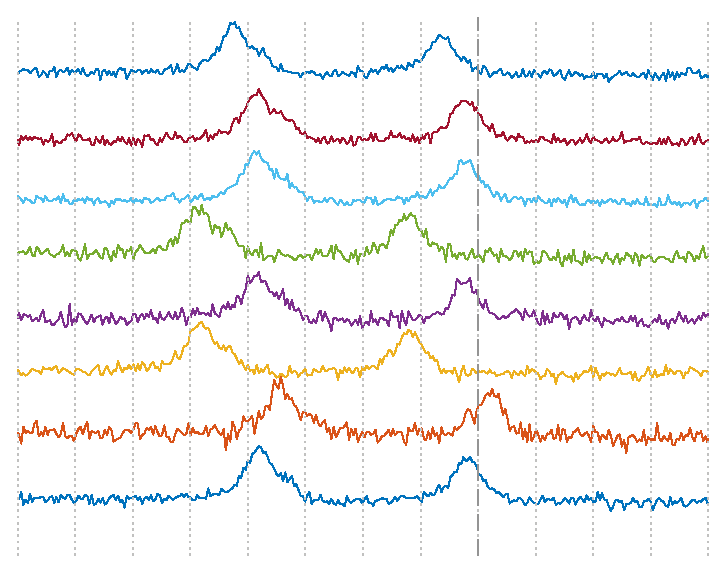
\includegraphics[width=0.95\textwidth, keepaspectratio]{images/samples_transients/8coil_wo_phase_w_fshift_cropped.eps}
        \caption{Phase alignment}
        \label{subfig:phase alignment}        
    \end{subfigure}
    \begin{subfigure}{0.32\textwidth}
        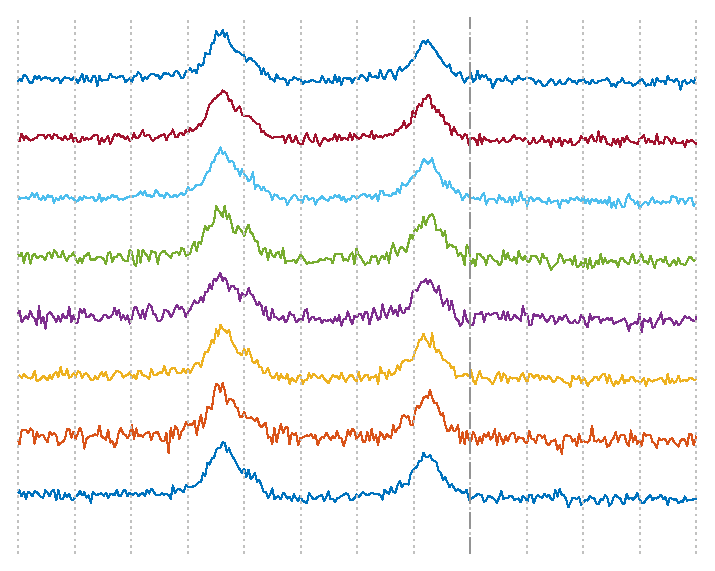
\includegraphics[width=0.95\textwidth, keepaspectratio]{images/samples_transients/8coil_wo_phase_wo_fshift_cropped.eps}
        \caption{Frequency alignment}
        \label{subfig:frequency alignment}        
    \end{subfigure}
    \caption{Examples of 8 simulated coil transients for a 3T GE PRESS sequence with TE=30ms. \ref{subfig:raw transients} shows transients with various SNRs and coil sensitivities along with zero-order phase and frequency offsets. \ref{subfig:phase alignment} shows the transients after phase alignment. \ref{subfig:frequency alignment} shows the transients after frequency alignment. After \ref{subfig:frequency alignment}, the transients can be averaged together and the coil-combined spectrum can then be fitted.}
    \label{fig:simulated transients}
\end{figure}

 
\paragraph{Coil Sensitivity}
A variety of coil combination techniques can be used to successfully combine multi-coil spectra. While these techniques differ in how they calculate the weights, all of them use weights to scale the transients before averaging. Assigning context, such as water peak height or coil sensitivity maps, to these weights when planning the simulations can help define the necessary parameter ranges and distributions to be in line with a given acquisition protocol.
 
\subsubsection{Final Steps} The desired use case will determine if a FID or a spectrum is necessary. If a FID is required, the simulation is finished and the data will be exported. If a spectrum is required, the Fourier transform will recover the spectrum at which point it can be cropped and resampled to a desired ppm range and spectral length. The default interpolation technique in this framework is a cubic Hermite modified Akima interpolator with momentum.


\subsection{Exporting Data}\label{subsec:exporting data}
The default export file format is .mat. These files include the data, spectral fits, simulation parameters, baseline offsets, and quantification results. To facilitate using the simulated spectra in various software packages, they are also exported in the NIfTI-MRS format\cite{Clarke2022}.
 
\subsection{Fitting Parameter Analysis}\label{subsec:Fitting Parameter Analysis}
The process of simulating a new dataset requires careful consideration of various factors, including the selection of appropriate parameter ranges and distributions. The optimal customization of these parameters depends on the intended use and application of the dataset. For instance, deep learning-based quantification models benefit from independent, uniform distributions that include all values the model will be expected to encounter. When validating a traditional spectral fitting model that includes soft constraints, it is crucial to incorporate those constraints when defining the parameter distributions. This ensures that the simulated dataset accurately reflects the underlying distribution of the target dataset. 

To mimic an in vivo dataset, accurate descriptions of clinical fitting parameters are crucially important. In collaboration with Osprey, it is now possible to export the spectral fitting parameters after quantification. Tools in this framework can then load the exported files and prepare the data for further analysis. Currently, this framework uses the python library Fitter\cite{Cokelaer2019} to identify the best fitting probability distribution for every parameter. \textit{A priori} knowledge, either from prior knowledge or data exploration, can narrow down the search range and speed up the analysis. The outputs for each parameter include evaluation metrics for the best performing distributions as well as a numerical characterization of the best fitting distribution.
 
\subsubsection{Recommendations}
The authors generally recommend that simulations include all relevant artifacts unless there is a specific reason to exclude them. A simulated dataset should include all phenomena that are expected to be encountered when the final work is deployed. Even highly accurate post-processing techniques have limitations and biases and leave some residue of the corrected artifacts. To ensure consistency between the simulated and clinical data, the artifacts should be included in the simulations and removed via the users’ own fitting protocols.  

Although not recommended, residual artifacts and post-processing techniques can be included in the simulations. Phase and frequency corrections can be simulated by applying a minimal offset during the initial simulation, which can be implemented in the parameter sampling protocol. Similarly, eddy currents can be scaled down by minimizing the sampled amplitudes. While not part of the acquisition protocol, apodization and zero filling are also possible. Apodization improves the SNR by multiplying the FID by a filter function, typically an exponential decay function or a Lorenztian-to-Gaussian transform. This framework implements an exponential decay as a function of time, $t$, and $T_L$ which defines the amount of apodization in Hz. Zero filling simply pads the FID with zeros to a defined length before the Fourier transform.

\subsection{Code}
This repository was written in PyTorch 1.11.0 and Python 3.9.7. Since this framework generates batches of spectra instead of individual spectra sequentially, a simulation batch size needs to be specified which will be affected by the spectral length and complexity of the simulations. As long as the batch size is set appropriately given the users' amount of RAM, this framework can be employed on standard computers without any special hardware. After publication, the repository will be available on GitHub, at \todo{https://www.github.com/REPOSITORY}, and MRSHub.


\section{Results}\label{sec:Results}
The selection of simulations presented in this section focus on short echo (TE=30ms) 3T PRESS spectra with a spectral width of 2000Hz and randomly sampled parameters. The concentrations were sampled with respect to total creatine (tCr). The choice of short echo spectra is motivated by their ability to capture a broader range of metabolite peaks compared to long echo spectra. The simulations presented include metabolites sampled from a comprehensive set of common brain metabolites including Asc, Asp, Ch, Cr, GABA, Gln, Glu, GPC, GSH, Lac, mI, NAA, NAAG, PCh, PCr, PE, sI, Tau, and a variety of macromolecular and lipid basis functions. For consistency, the SNR was fixed to 15dB and the chemical shift reference point is set to 4.65ppm.

It is important to note that while pulse sequence implications are integral to the overall simulation process, their detailed exploration is beyond the scope of this work. Therefore, in this study, the simulations are specifically tailored to the PRESS sequence. 
% While the pulse sequence implications are acknowledged as an important aspect of MRS simulations, their exploration is beyond the immediate scope of this work. 
The main objective of this work is to manipulate pre-simulated basis sets until they approximate in vivo spectra. Therefore, the primary machinations of MRS-Sim are the same regardless of the basis functions used. Overall, the presented simulations using the PRESS sequence provide a valuable foundation for understanding the performance and capabilities of the MRS-Sim framework.

\subsection{Baseline and Residual Water Generator}
\begin{figure}[t!]
    \centering
    \begin{tabular}[c]{ccc}
    \begin{subfigure}[c]{0.31\textwidth}
        \includegraphics[width=0.93\textwidth,keepaspectratio]{images/30ms_samples/curated/30ms_curated_sample{1}.eps}
        \vspace{3pt}
    \end{subfigure}&
    \begin{subfigure}[c]{0.31\textwidth}
        \includegraphics[width=0.93\textwidth,keepaspectratio]{images/30ms_samples/curated/30ms_curated_sample{2}.eps}
        \vspace{3pt}
    \end{subfigure}&
    \begin{subfigure}[c]{0.31\textwidth}
        \includegraphics[width=0.93\textwidth,keepaspectratio]{images/30ms_samples/curated/30ms_curated_sample{3}.eps}
        \vspace{3pt}
    \end{subfigure}\\
    \begin{subfigure}[c]{0.31\textwidth}
        \includegraphics[width=0.93\textwidth,keepaspectratio]{images/30ms_samples/curated/30ms_curated_sample{4}.eps}
        \vspace{3pt}
    \end{subfigure}&
    \begin{subfigure}[c]{0.31\textwidth}
        \includegraphics[width=0.93\textwidth,keepaspectratio]{images/30ms_samples/curated/30ms_curated_sample{5}.eps}
        \vspace{3pt}
    \end{subfigure}&%
    \begin{subfigure}[c]{0.31\textwidth}
        \includegraphics[width=0.93\textwidth,keepaspectratio]{images/30ms_samples/curated/30ms_curated_sample{6}.eps}
        \vspace{3pt}
    \end{subfigure}\\
    \begin{subfigure}[c]{0.31\textwidth}
        \includegraphics[width=0.93\textwidth,keepaspectratio]{images/30ms_samples/curated/30ms_curated_sample{7}.eps}
        \vspace{3pt}
    \end{subfigure}&
    \begin{subfigure}[c]{0.31\textwidth}
        \includegraphics[width=0.93\textwidth,keepaspectratio]{images/30ms_samples/curated/30ms_curated_sample{8}.eps}
        \vspace{3pt}
    \end{subfigure}&
    \begin{subfigure}[c]{0.31\textwidth}
        \includegraphics[width=0.93\textwidth,keepaspectratio]{images/30ms_samples/curated/30ms_curated_sample{9}.eps}
        \vspace{3pt}
    \end{subfigure}\\
    \begin{subfigure}[c]{0.31\textwidth}
        \includegraphics[width=0.93\textwidth,keepaspectratio]{images/30ms_samples/curated/30ms_curated_sample{10}.eps}
        \vspace{3pt}
    \end{subfigure}&
    \begin{subfigure}[c]{0.31\textwidth}
        \includegraphics[width=0.93\textwidth,keepaspectratio]{images/30ms_samples/curated/30ms_curated_sample{11}.eps}
        \vspace{3pt}
    \end{subfigure}&%
    \begin{subfigure}[c]{0.31\textwidth}
        \includegraphics[width=0.93\textwidth,keepaspectratio]{images/30ms_samples/curated/30ms_curated_sample{12}.eps}
        \vspace{3pt}
    \end{subfigure}\\
    \begin{subfigure}[c]{0.31\textwidth}
        \includegraphics[width=0.93\textwidth,keepaspectratio]{images/30ms_samples/curated/30ms_curated_sample{13}.eps}
    \end{subfigure}&
    \begin{subfigure}[c]{0.31\textwidth}
        \includegraphics[width=0.93\textwidth,keepaspectratio]{images/30ms_samples/curated/30ms_curated_sample{14}.eps}
    \end{subfigure}&%
    \begin{subfigure}[c]{0.31\textwidth}
        \includegraphics[width=0.93\textwidth,keepaspectratio]{images/30ms_samples/curated/30ms_curated_sample{15}.eps}
    \end{subfigure}
    \end{tabular}
    \caption{Sample spectra simulated for a PRESS sequence with TE=30ms that highlight the effect of the baseline and residual water contributions.}
    \label{fig:30ms samples curated clean}
\end{figure}


Fig. \ref{fig:30ms samples curated clean} illustrates a single clean short echo (TE=30ms) PRESS spectrum showcasing various combinations of residual water and baseline contributions. The metabolite concentrations and lineshapes were fixed in addition to the settings described above. These samples omit spectral artifacts to more clearly highlight the variety that can be achieved by randomly sampling parameters for the baseline and residual water generator. 

It should be noted that it is currently unknown what a true baseline looks like. Different baseline modeling protocols produce different baselines and because in vivo data does not have known ground truths, there is no way to identify which method is the most correct. Because of this, the proposed generator produces a wide variety of baselines that approximate the baselines extracted by traditional methods. The motivation behind this approach is the idea that if the generator cannot be limited to strictly in vivo-like baselines, then it should incorporate a variety of appropriate baseline profiles such that true baselines are included. Because this generator is not based on a baseline fitting method, future work could use it to evaluate the baseline modeling performance of various fitting protocols given different baseline profiles.

\subsection{Complete Model}
In contrast, Fig. \ref{fig:30ms samples curated dirty} presents a simulated PRESS spectrum (TE=30ms) with randomly sampled artifacts, and offsets. %The dropout probability for each parameter was set to 50\%. This means that the model parameters, including metabolites, are randomly omitted from the simulations. This helps to emphasize the variety of outputs that are possible for a single set of defined ranges and distributions. 
This figure highlights the variety a single spectrum can assume just by randomly sampling the artifacts. Sophisticated simulations, such as these, are useful for developing and validating data processing techniques such as artifact removal and new spectral fitting protocols. Spectra can be simulated to be as clean or as dirty as desired, all while maintaining known ground truth values. %Because every component in these simulations has a known ground truth, even the most challenging spectra can 



It should be noted that the baselines and residual water regions shown sometimes appear to be uncorrelated with the depicted spectra. This is due to additional artifacts that are applied to the simulations after all of the spectral components are combined. The plotted baseline and residual water regions are the ground truths and do not have additional artifacts applied to them. %Sophisticated simulations, such as these, are useful for developing and validating artifact removal techniques and spectral fitting protocols.  
\begin{figure}[ht!]
    \centering
    \begin{tabular}[c]{ccc}
    \begin{subfigure}[c]{0.31\textwidth}
        \includegraphics[width=0.93\textwidth]{images/30ms_samples/dirty/30ms_curated_dirty_sample{1}.eps}
        \vspace{3pt}
    \end{subfigure}&
    \begin{subfigure}[c]{0.31\textwidth}
        \includegraphics[width=0.93\textwidth]{images/30ms_samples/dirty/30ms_curated_dirty_sample{2}.eps}
        \vspace{3pt}
    \end{subfigure}&
    \begin{subfigure}[c]{0.31\textwidth}
        \includegraphics[width=0.93\textwidth]{images/30ms_samples/dirty/30ms_curated_dirty_sample{3}.eps}
        \vspace{3pt}
    \end{subfigure}\\
    \begin{subfigure}[c]{0.31\textwidth}
        \includegraphics[width=0.93\textwidth]{images/30ms_samples/dirty/30ms_curated_dirty_sample{4}.eps}
        \vspace{3pt}
    \end{subfigure}&
    \begin{subfigure}[c]{0.31\textwidth}
        \includegraphics[width=0.93\textwidth]{images/30ms_samples/dirty/30ms_curated_dirty_sample{5}.eps}
        \vspace{3pt}
    \end{subfigure}&%
    \begin{subfigure}[c]{0.31\textwidth}
        \includegraphics[width=0.93\textwidth]{images/30ms_samples/dirty/30ms_curated_dirty_sample{6}.eps}
        \vspace{3pt}
    \end{subfigure}\\
    \begin{subfigure}[c]{0.31\textwidth}
        \includegraphics[width=0.93\textwidth]{images/30ms_samples/dirty/30ms_curated_dirty_sample{7}.eps}
        \vspace{3pt}
    \end{subfigure}&
    \begin{subfigure}[c]{0.31\textwidth}
        \includegraphics[width=0.93\textwidth]{images/30ms_samples/dirty/30ms_curated_dirty_sample{8}.eps}
        \vspace{3pt}
    \end{subfigure}&
    \begin{subfigure}[c]{0.31\textwidth}
        \includegraphics[width=0.93\textwidth]{images/30ms_samples/dirty/30ms_curated_dirty_sample{9}.eps}
        \vspace{3pt}
    \end{subfigure}\\
    \begin{subfigure}[c]{0.31\textwidth}
        \includegraphics[width=0.93\textwidth]{images/30ms_samples/dirty/30ms_curated_dirty_sample{10}.eps}
        \vspace{3pt}
    \end{subfigure}&
    \begin{subfigure}[c]{0.31\textwidth}
        \includegraphics[width=0.93\textwidth]{images/30ms_samples/dirty/30ms_curated_dirty_sample{11}.eps}
        \vspace{3pt}
    \end{subfigure}&%
    \begin{subfigure}[c]{0.31\textwidth}
        \includegraphics[width=0.93\textwidth]{images/30ms_samples/dirty/30ms_curated_dirty_sample{12}.eps}
        \vspace{3pt}
    \end{subfigure}\\
    \begin{subfigure}[c]{0.31\textwidth}
        \includegraphics[width=0.93\textwidth]{images/30ms_samples/dirty/30ms_curated_dirty_sample{13}.eps}
    \end{subfigure}&
    \begin{subfigure}[c]{0.31\textwidth}
        \includegraphics[width=0.93\textwidth]{images/30ms_samples/dirty/30ms_curated_dirty_sample{14}.eps}
    \end{subfigure}&%
    \begin{subfigure}[c]{0.31\textwidth}
        \includegraphics[width=0.93\textwidth]{images/30ms_samples/dirty/30ms_curated_dirty_sample{15}.eps}
    \end{subfigure}\\
    \end{tabular}
    \caption{Sample spectra, similar to Fig. \ref{fig:30ms samples curated clean} [PRESS, TE=30ms], with randomly sampled, uncorrected artifacts to approximate raw data.}%Sample spectra simulated for a PRESS sequence with TE=30ms. These spectra have sampled parameters just like Fig. \ref{fig:30ms samples curated clean} plus a variety of uncorrected artifacts including eddy currents, zero- and first-order phase offsets, frequency shifts, macromolecule and lipid contributions, residual water, and baseline offsets.}
    \label{fig:30ms samples curated dirty}
\end{figure}




\section{Discussion}\label{sec:discussion}
This work presents a flexible, open-source framework to help researchers generate complex, in vivo-like MRS data. Spectral components from state-of-the-art spectral fitting models were combined to create a comprehensive model. Flexibility and modularity are key components that make this framework a viable option for simulating in vivo-like data representing a multitude of clinical scenarios.

The use of synthetic MRS data has become increasingly popular in recent years due to the need for large datasets with known spectral components. Using synthetic data allows researchers to create unlimited spectra with known ground truth values. This is useful for both traditional spectroscopy and deep learning applications, including evaluating the accuracy and precision of data analysis methods. However, there is a lack of standardization in synthetic data generation, which poses challenges in terms of reproducibility and generalizability.

Researchers currently use a variety of simulation frameworks to generate synthetic data for their particular needs. These frameworks often involve simplifying assumptions regarding the spectral components, which excludes some components that are deemed non-essential for that particular task. These assumptions make synthetic data less generalizable, similar to phantom data which struggles to approximate in vivo data. In general, simulating data has two primary challenges: which spectral components and artifacts to include and what parameter values to use for the included components. These choices can be difficult for experts, let alone non-expert users. Moreover, the heterogeneity in the simulation methods used makes reproducibility challenging.
 
MRS-Sim addresses these challenges as an open-source solution for a synthetic data generation model that includes a comprehensive list of spectral components and acquisition-induced artifacts. Several novel contributions are presented to include experimental artifacts that are usually ignored during spectral modeling. These modules are designed to make the simulations more comprehensive and in vivo-like. The first contribution is a $B_0$ field simulator. It is capable of introducing distortions due to imperfect shimming and high susceptibility effects into the simulations. Then, a semi-parametric generator is proposed that can simulate both broad, undulating baseline offsets and highly irregular residual water contributions. The implementation of the presented framework is flexible and can be updated with new information as research progresses to improve the realness and accuracy of the simulations. 

The modularity of the MRS-Sim implementation is one of its key features, allowing for flexible and customizable use of the framework. Firstly, the functions that add artifacts and spectral components are modular and independent, which makes it very easy to understand the code and its purpose. Secondly, it allows for the easy generation of highly customized datasets for various clinical scenarios, as the simulation step itself is also modular. Consequently, this feature enables easy community contributions to develop new functionalities, thus preventing the need for entirely new frameworks. New scenarios, such as J-difference edited spectra, diffusion spectra, or 2D spectra, can be developed and seamlessly integrated.

The appendix and digital repository include a table that provides up-to-date information about moiety- and metabolite-level characterizations of things like spin-systems, temperature-induced artifacts, $T_2$ values, and metabolite concentration ranges. This information can be continually updated to provide the community with comprehensive and state-of-the-art information about brain metabolites at a glance. Additionally, these suggested values provide a good starting point for simulating datasets. Cumulatively, this framework offers a pathway to generate realistic, in vivo-like synthetic data that captures acquisition-induced artifacts and nuisance signals and can be applied across a range of MRS applications. 
\section{Discussions}\label{sec:Conclusions}
The use of synthetic MRS data has gained significant interest in recent years due to the need for large datasets with known spectral components for both traditional spectroscopy and deep learning applications. Synthetic data allows researchers to generate unlimited spectra with known ground truth values which has wide-ranging applications, including evaluating the accuracy and precision of data analysis methods. However, the lack of standardization in synthetic data generation poses challenges in terms of reproducibility and generalizability.

As discussed in the introduction, researchers currently use a variety of simulation frameworks to generate synthetic data for their particular need. Oftentimes these include simplifying assumptions for the spectral components considered non-essential for their task. These assumptions limit the generalizability of synthetic data in the same way phantom data struggles to approximate in vivo data. In general, simulating data has two primary challenges: what spectral components and artifacts to include, and what parameter values to use for the included components. Such choices can be challenging, even for expert users, making much of this out of reach for non-expert users. In addition to being challenging to simulate, such heterogeneity in the simulation methods complicates reproducibility.%Even expert users can struggle to find appropriate values. 
% And much like simulating a basis set for a custom pulse sequence requires knowledge that is generally unavailable to non-expert users, in vivo-like simulations can also be 

 
To address these issues, this work has presented an open-source framework for a modular synthetic data generation model. %Standard spectral artifacts have been incorporated and can be easily applied. 
A comprehensive list of spectral components and acquisition-induced artifacts were incorporated. 
Several novel contributions are proposed to include experimental artifacts that are traditionally overlooked during spectral modeling, making these simulations comprehensive and in vivo-like. The first is a $B_0$ magnetic field simulator that is capable of introducing distortions due to imperfect shimming and high susceptibility effects into the simulations. Then, a novel generator was proposed that is capable of simulating both broad, undulating baseline offsets and highly irregular residual water contributions. This framework was intentionally designed so that as research progresses, new information can be added to further improve the realness and accuracy of the simulations. To further that point, a table of has been compiled in the appendix and the repository that provides up-to-date moiety- and metabolite-level characterizations of things like spin-systems, temperature-induced artifacts, T2 values, and metabolite concentration ranges. This can be continually updated to provide the community with comprehensive and state-of-the-art information about brain metabolites at a glance. Additionally, these suggested values provide a good starting point for simulating datasets. Cumulatively, this offers a pathway to generate realistic, in vivo-like synthetic data that captures acquisition-induced artifacts and nuisance signals, and can be applied across a range of MRS applications. 

The modularity of MRS-Sim is another key feature of this framework. First and foremost is that modularity of the functions adding artifacts and spectral components makes it very easy to look at the code and understand what it is doing. Secondly, it allows for the easy generation of highly tailored datasets for a variety of clinical scenarios because the simulation step itself is also modular. Consequently, this makes it easy for community contributions to further develop new functionalities. The authors believe this is a crucial aspect %to promote wide-spread adoption 
because it won't leave a gap that needs to be filled by entirely new frameworks. New scenarios, such as J-difference edited spectra, diffusion spectra, or, eventually, 2D spectra, can be developed and seamlessly integrated.
 
The development of open-source frameworks for data generation are crucial for ensuring widespread adoption and improving the generalizability of synthetic MRS data and the reproducibility of MRS research. By open-sourcing this work, the authors aim to contribute to the democratization of MRS research by providing access to high quality information and simulations to a wider community of researchers interested in the field. Improving the quality of synthetic data inherently improves its generalizability to in vivo data with the natural consequence being improved overall applicability of synthetic data in MRS. Furthermore, this will promote greater standardization and reproducibility. Moving forward, collaboration and consensus-building among researchers will be essential to establish standards and best practices for simulating MRS data. As mentioned above, future development can focus on adding additional clinical scenarios to the framework's repertoire, increasing its applicability to even more aspects of MRS. Further research can use this framework to, for example, compare the impact of different spectral modeling components on metabolite quantification or to compare the performance of commonly used spectral fitting models. By addressing the challenges associated with synthetic MRS data generation and promoting standardization, MRS can continue to advance in every aspect of the field. 


\newacronym{ML}{ML}{machine learning}
\newacronym{DL}{DL}{deep learning}
\newacronym{Asc}{Asc}{ascorbate}
\newacronym{Asp}{Asp}{aspartate}
\newacronym{Ch}{Ch}{choline}
\newacronym{Cr}{Cr}{creatine}
\newacronym{GABA}{GABA}{gamma-aminobutyric acide}
\newacronym{Gln}{Gln}{glutamine}
\newacronym{Glu}{Glu}{glutamate}
\newacronym{GPC}{GPC}{glycerophosphorylcholine}
\newacronym{GSH}{GSH}{glutathione}
\newacronym{Lac}{Lac}{lactate}
\newacronym{mI}{mI}{myo-inositol}
\newacronym{NAA}{NAA}{N-acetylaspartate}
\newacronym{NAAG}{NAAG}{N-acetylaspartylglutamate}
\newacronym{PCh}{PCh}{phosphocholine}
\newacronym{PCr}{PCr}{phosphocreatine}
\newacronym{PE}{PE}{phosphatidylethanolamine}
\newacronym{sI}{sI}{scyllo-inositol}
\newacronym{Tau}{Tau}{taurine}
\newacronym{tCr}{tCr}{total Creatine}
% \newacronym{FID}{FID}{free induction decay}
% \newacronym{ppm}{ppm}{parts per million}
% \newacronym{SNR}{SNR}{signal-to-noise ratio}
% \newacronym{RAM}{RAM}{random access memory}
% \newacronym{std}{std}{standard deviation}
% \newacronym{MRS}{MRS}{magnetic resonance spectroscopy}
\newacronym{PRESS}{PRESS}{point resolved spectroscopy}
% \newacronym{MRI}{MRI}{magnetic resonance imaging}
\newacronym{STEAM}{STEAM}{stimulated echo acquisition method}
% \newacronym{TE}{TE}{echo time}
% \newacronym{Hz}{Hz}{hertz}
% \newacronym{dB}{dB}{decibel}
\newacronym{MARSS}{MARSS}{Magnetic Resonance Spectrum Simulator}
\newacronym{LASER}{LASER}{localized adiabatic selective refocusing}
\newacronym{sLASER}{sLASER}{semi-localized adiabatic selective refocusing}
\glsaddall
\section*{Abbreviations}
\begin{multicols}{3}
\printglossary[type=\acronymtype, nonumberlist]
\end{multicols}

\section*{Acknowledgments}
The authors would like to thank Dr. Tobias Lasser for his mentorship during this work; Dr. Dhritiman Das for discussions about his experience with simulating MRS SVS data; the Harper House for their support while visiting UCSF to further develop the physics model; and the DAAD and Technical University of Munich's Graduate Center of Computation, Information and Technology for helping to finance the stay at UCSF in San Francisco, USA.

\subsection*{Funding Information}
This work was supported in part by a doctoral fellowship from the German Academic Exchange Service (DAAD) and the following grants from the National Institutes of Health: R00 AG062230, R01 CA262630, and R21 EB033516.

\subsection*{Conflict of interest}
The authors declare no potential conflict of interest.

% \input{sections/supplement.tex}


%\nocite{*}% Show all bib entries - both cited and uncited; comment this line to view only cited bib entries;
\bibliography{mybibliography}

% \clearpage
% % \begin{longtable*}
% \begin{tabular}
\begin{longtable*}{cccccccccccccccccccccccccccccccc}
% & & & & \multicolumn{24}{c}{ Literature } & \multicolumn{4}{c}{Recommendations}     \\
\multirow{2}{*}{ Name } & 
\multirow{2}{*}{ Abbr. } & 
\multirow{2}{*}{ Moieties } & 
\multirow{2}{*}{ Group } & 
\multirow{2}{*}{ \thead[c]{Chemical Shift \\ (ppm) [2-3]} } & 
\multirow{2}{*}{ \thead[c]{Chemical Shift \\ (ppm) [8]} } & 
\multirow{2}{*}{ \thead[c]{Chemical Shift \\ (ppm) [4-5]} } & 
\multirow{2}{*}{ \thead[c]{Multiplicity \\ $[2-3]$} } & 
\multirow{2}{*}{ \thead[c]{Multiplicity \\ $[4-5]$} } & 
% \multirow{2}{*}{ \thead[c]{Multiplicity \\ [2-3]} } & 
% \multirow{2}{*}{ \thead[c]{Multiplicity \\ [4-5]} } & 
\multirow{2}{*}{ Interaction } & 
\multirow{2}{*}{ \thead[c]{Scalar coupling \\ (Hz) [2-3]} } & 
\multirow{2}{*}{ \thead[c]{Scalar coupling \\ (Hz) [8]} } & 
\multirow{2}{*}{ \thead[c]{Scalar coupling \\ (Hz) [4-5]} } & 
\multicolumn{3}{c}{\thead[c]{Temperature-induced \\Frequency shift [10]}} & 
\multicolumn{6}{c}{T2 [ms] ± STD [11]} & 
\multicolumn{2}{c}{T2 [ms] [6]} & 
\multicolumn{2}{c}{Concentrations [mM] [6]} & 
\multicolumn{2}{c}{Concentrations [mM] [2]} & 
\multicolumn{2}{c}{T2 [ms]} & 
\multicolumn{2}{c}{Concentrations [mM]}                  \\

& & & & & & & & & & & & & Slope [e\textsuperscript{-4} ppm/C] & STD & b [ppm] & \multicolumn{2}{c}{PVWM} & \multicolumn{2}{c}{OCC} & \multicolumn{2}{c}{pACC} & Low & High & Low & High & Low & High & Low & High & Low & High        \\
Acetate & Ace & \textemdash & \textsuperscript{2}CH\textsubscript{3} & 1.904 & 1.9040 & 1.9040 & s & s & \textemdash & \textemdash & \textemdash & \textemdash & \textemdash & \textemdash & \textemdash & \textemdash & \textemdash & \textemdash & \textemdash & \textemdash & \textemdash & 0 & 0 & 0 & 0 & 0 & 0.5 & \textemdash & \textemdash & \textemdash & \textemdash \\
\multirow{4}{*}{ Alanine } & \multirow{4}{*}{ Ala } & \multirow{4}{*}{ \textemdash } & \textsuperscript{2}CH & 3.775 & 3.7750 & 3.7746 & q & q & 2-3 & 7.23 & 7.230 & 7.230 & 1.5402 & 0.2368 & -0.0057 & \textemdash & \textemdash & \textemdash & \textemdash & \textemdash & \textemdash & \multirow{4}{*}{ 100 } & \multirow{4}{*}{ 250 } & \multirow{4}{*}{ 0.000 } & \multirow{4}{*}{ 0.000 } & \multirow{4}{*}{ 0.100 } & \multirow{4}{*}{ 1.500 } & 100.000 & 250.000 & \multirow{4}{*}{ 0.090 } & \multirow{4}{*}{ 1.650 }     \\
& & & \textsuperscript{3}CH\textsubscript{3} & 1.467 & 1.4667 & 1.4667 & d & d & 3-3' & \textemdash & \textemdash & -14.366 & \textemdash & \textemdash & \textemdash & \textemdash & \textemdash & \textemdash & \textemdash & \textemdash & \textemdash & & & & & & & 100.000 & 250.000 & & \\
& & & & \textemdash & \textemdash & \textemdash & \textemdash & \textemdash & 3-3'' & \textemdash & \textemdash & -14.366 & & & & \textemdash & \textemdash & \textemdash & \textemdash & \textemdash & \textemdash & & & & & & & 100.000 & 250.000 & & \\
& & & & \textemdash & \textemdash & \textemdash & \textemdash & \textemdash & 3'-3'' & \textemdash & \textemdash & -14.366 & & & & \textemdash & \textemdash & \textemdash & \textemdash & \textemdash & \textemdash & & & & & & & 100.000 & 250.000 & & \\
\multirow{4}{*}{ Ascorbic Acid } & \multirow{4}{*}{ Asc } & \multirow{4}{*}{ \textemdash } & \textsuperscript{4}CH & 4.492 & 4.4920 & 4.4920 & d & d & 4-5 & 2.07 & 2.07 & 2.07 & \textemdash & \textemdash & \textemdash & 172 & 25 & 105 & 16 & 125 & 19 & \multirow{4}{*}{ 100 } & \multirow{4}{*}{ 250 } & \multirow{4}{*}{ 0.408 } & \multirow{4}{*}{ 1.883 } & \multirow{4}{*}{ 0.500 } & \multirow{4}{*}{ 1.500 } & 73.000 & 250.000 & \multirow{4}{*}{ 0.367 } & \multirow{4}{*}{ 2.072 }     \\
& & & \textsuperscript{5}CH & 4.002 & 4.0020 & 4.0020 & m & m & 5-6 & 6.00 & 6.00 & 6.00 & \textemdash & \textemdash & \textemdash & 172 & 25 & 105 & 16 & 125 & 19 & & & & & & & 73.000 & 250.000 & & \\
& & & \textsuperscript{6}CH\textsubscript{2} & 3.743 & 3.7430 & 3.7430 & m & m & 5-6' & 7.60 & 7.60 & 7.60 & \textemdash & \textemdash & \textemdash & 172 & 25 & 105 & 16 & 125 & 19 & & & & & & & 73.000 & 250.000 & & \\
& & & & 3.716 & 3.7160 & 3.7160 & \textemdash & \textemdash & 6-6' & -11.50 & -11.50 & -11.50 & \textemdash & \textemdash & \textemdash & 172 & 25 & 105 & 16 & 125 & 19 & & & & & & & 73.000 & 250.000 & & \\
\multirow{3}{*}{ Aspartate } & \multirow{3}{*}{ Asp } & \multirow{3}{*}{ \textemdash } & \textsuperscript{2}CH & 3.891 & 3.8914 & 3.8914 & dd & dd & 2-3 & 3.65 & 3.647 & 3.647 & -0.0691 & 0.1863 & 0.0003 & 148 & 21 & 90 & 27 & 111 & 20 & \multirow{3}{*}{ 120.15 } & \multirow{3}{*}{ 204.55 } & \multirow{3}{*}{ 0.000 } & \multirow{3}{*}{ 6.971 } & \multirow{3}{*}{ 1.000 } & \multirow{3}{*}{ 2.000 } & 36.000 & 204.550 & \multirow{3}{*}{ 0.900 } & \multirow{3}{*}{ 7.668 }     \\
& & & \textsuperscript{3}CH\textsubscript{2} & 2.804 & 2.8011 & 2.8021 & dd & dd & 2-3' & 9.11 & 9.107 & 9.107 & 4.1970 & 0.1913 & -0.0155 & 148 & 21 & 90 & 27 & 111 & 20 & & & & & & & 36.000 & 204.550 & & \\
& & & & 2.670 & 2.6533 & 2.6508 & dd & dd & 3-3' & -17.43 & -17.426 & -17.426 & 4.1970 & 0.1913 & -0.0155 & 148 & 21 & 90 & 27 & 111 & 20 & & & & & & & 36.000 & 204.550 & & \\
\multirow{5}{*}{ \thead[c]{2-Hydroxy- \\glutarate [1]} } & \multirow{5}{*}{ \thead[c]{aHG \\ 2HG} } & \multirow{5}{*}{ \textemdash } & \textsuperscript{2}CH & 4.022 & 4.0220 & 4.0220 & dd & dd & 2-3 / 2-3' & 7.65 / 4.04 & 7.600 / 4.100 & 7.600 / 4.100 & \textemdash & \textemdash & \textemdash & \textemdash & \textemdash & \textemdash & \textemdash & \textemdash & \textemdash & \multirow{5}{*}{ 0 } & \multirow{5}{*}{ 0 } & \multirow{5}{*}{ 0.000 } & \multirow{5}{*}{ 0.000 } & \multirow{5}{*}{ \textemdash } & \multirow{5}{*}{ \textemdash } & \textemdash & \textemdash & \multirow{5}{*}{ \textemdash } & \multirow{5}{*}{ \textemdash }         \\
& & & \textsuperscript{3}CH\textsubscript{2} & 1.825 & 1.8250 & 1.8250 & m & m & 3-3' & -14.00 & -14.000 & -14.000 & \textemdash & \textemdash & \textemdash & \textemdash & \textemdash & \textemdash & \textemdash & \textemdash & \textemdash & & & & & & & \textemdash & \textemdash & & \\
& & & & 1.977 & 1.9770 & 1.9770 & m & m & 3-4 / 3-4' & 5.25 / 10.66 & 5.300 / 10.400 & 5.300 / 10.400 & \textemdash & \textemdash & \textemdash & \textemdash & \textemdash & \textemdash & \textemdash & \textemdash & \textemdash & & & & & & & \textemdash & \textemdash & & \\
& & & \textsuperscript{4}CH\textsubscript{2} & 2.221 & 2.2210 & 2.2210 & m & m & 3'-4 / 3'-4' & 10.84 / 5.86 & 10.600 / 6.000 & 10.600 / 6.000 & \textemdash & \textemdash & \textemdash & \textemdash & \textemdash & \textemdash & \textemdash & \textemdash & \textemdash & & & & & & & \textemdash & \textemdash & & \\
& & & & 2.272 & 2.2720 & 2.2720 & m & m & 4-4' & -14.91 & -15.000 & -15.000 & \textemdash & \textemdash & \textemdash & \textemdash & \textemdash & \textemdash & \textemdash & \textemdash & \textemdash & & & & & & & \textemdash & \textemdash & & \\
\multirow{5}{*}{ Choline } & \multirow{5}{*}{ Ch } & \multirow{5}{*}{ \textemdash } & N(CH\textsubscript{3})\textsubscript{3} & 3.185 & 3.1850 & 3.1850 & s & s & \textemdash & \textemdash & 0.570 & \textemdash & \textemdash & \textemdash & \textemdash & 213 & 25 & 221 & 51 & 274 & 60 & \multirow{5}{*}{ \textemdash } & \multirow{5}{*}{ \textemdash } & \multirow{5}{*}{ 0.000 } & \multirow{5}{*}{ 0.000 } & \multirow{5}{*}{ 0.5 (total) } & \multirow{5}{*}{ 2.5 (total) } & 119.000 & 394.000 & \multirow{5}{*}{ 0.000 } & \multirow{5}{*}{ 2.750 }     \\
& & & \textsuperscript{1}CH\textsubscript{2} & 4.054 & 4.0540 & 4.0540 & m & m & 1-2 / 1'-2' & 3.14 / 3.17 & 3.140 / 3.168 & 3.140 / 3.168 & \textemdash & \textemdash & \textemdash & 178 & 20 & 191 & 49 & 243 & 51 & & & & & & & 93.000 & 345.000 & & \\
& & & & & & & \textemdash & \textemdash & 1-1' & -14.10 & 2.572 & -14.100 & \textemdash & \textemdash & \textemdash & 178 & 20 & 191 & 49 & 243 & 51 & & & & & & & 93.000 & 345.000 & & \\
& & & \textsuperscript{2}CH\textsubscript{2} & 3.501 & 3.5010 & 3.5010 & m & m & 1'-2 / 1-2' & 7.01 / 6.98 & 7.011 / 6.979 & 7.011 / 6.979 & \textemdash & \textemdash & \textemdash & 178 & 20 & 191 & 49 & 243 & 51 & & & & & & & 93.000 & 345.000 & & \\
& & & & & & & \textemdash & \textemdash & 2-2' & -14.10 & 2.681 & -14.070 & \textemdash & & & 178 & 20 & 191 & 49 & 243 & 51 & & & & & & & 93.000 & 345.000 & & \\
\multirow{3}{*}{ Creatine } & \multirow{3}{*}{ Cr } & \multirow{3}{*}{ \textemdash } & N(CH\textsubscript{3}) & 3.027 & 3.0270 & 3.0270 & s & s & \textemdash & \textemdash & \textemdash & \textemdash & \textemdash & \textemdash & \textemdash & 166 & 11 & 144 & 17 & 148 & 22 & 164.08 & 242.7 & \multirow{3}{*}{ 0.361 } & \multirow{3}{*}{ 15.005 } & \multirow{3}{*}{ 4.500 } & \multirow{3}{*}{ 10.500 } & 104.000 & 242.700 & \multirow{3}{*}{ 0.325 } & \multirow{3}{*}{ 16.505 }    \\
& & & \textsuperscript{2}CH\textsubscript{2} & 3.913 & 3.9130 & 3.9130 & s & s & \textemdash & \textemdash & \textemdash & \textemdash & -6.2166 & 0.1158 & 0.0230 & 129 & 13 & 112 & 18 & 134 & 15 & 135.18 & 213.8 & & & & & 76.000 & 213.800 & & \\
& & & NH & 6.650 & 6.6490 & 6.6490 & s & s & \textemdash & \textemdash & \textemdash & \textemdash & \textemdash & \textemdash & \textemdash & \textemdash & \textemdash & \textemdash & \textemdash & \textemdash & \textemdash & 164.08 & 242.7 & & & & & 164.080 & 242.700 & & \\
\multirow{4}{*}{ Ethanolamine } & \multirow{4}{*}{ Eth } & \multirow{4}{*}{ \textemdash } & \textsuperscript{1}CH\textsubscript{2} & 3.818 & 3.8184 & 3.8184 & m & m & 1-2 / 1'-2' & 3.85 & 3.897 / 3.798 & 3.897 / 3.798 & \textemdash & \textemdash & \textemdash & \textemdash & \textemdash & \textemdash & \textemdash & \textemdash & \textemdash & \multirow{4}{*}{ \textemdash } & \multirow{4}{*}{ \textemdash } & \multirow{4}{*}{ 0.000 } & \multirow{4}{*}{ 0.000 } & \multirow{4}{*}{ 0.000 } & \multirow{4}{*}{ 1.500 } & \textemdash & \textemdash & \multirow{4}{*}{ 0.000 } & \multirow{4}{*}{ 1.650 }     \\
& & & & & & & \textemdash & \textemdash & 1-1' / 1-N & -10.20 / \textemdash & -10.640 / 0.657 & -10.640 / 0.657 & \textemdash & \textemdash & \textemdash & \textemdash & \textemdash & \textemdash & \textemdash & \textemdash & \textemdash & & & & & & & \textemdash & \textemdash & & \\
& & & \textsuperscript{2}CH\textsubscript{2} & 3.147 & 3.1467 & 3.1467 & m & m & 1'-2 / 1-2' & 6.75 & 6.694 / 6.794 & 6.694 / 6.794 & \textemdash & \textemdash & \textemdash & \textemdash & \textemdash & \textemdash & \textemdash & \textemdash & \textemdash & & & & & & & \textemdash & \textemdash & & \\
& & & & & & & \textemdash & \textemdash & 2-2' / 1'-N & -10.2 / \textemdash & -11.710 / 0.1420 & -11.710 / 0.1420 & \textemdash & \textemdash & \textemdash & \textemdash & \textemdash & \textemdash & \textemdash & \textemdash & \textemdash & & & & & & & \textemdash & \textemdash & & \\
\multirow{7}{*}{ \thead[c]{$\gamma$-Aminobutyric\\ acid} } & \multirow{7}{*}{ GABA } & \multirow{7}{*}{ \textemdash } & \textsuperscript{2}CH\textsubscript{2} & 2.287 & 2.2840 & 2.2840 & t & t & 2-2' & \textemdash & -15.938 & -10.744 & & & & & & & & & & \multirow{7}{*}{ 77.37 } & \multirow{7}{*}{ 161.77 } & \multirow{7}{*}{ 0.037 } & \multirow{7}{*}{ 9.745 } & \multirow{7}{*}{ 1.000 } & \multirow{7}{*}{ 2.000 } & \textemdash & \textemdash & \multirow{7}{*}{ 0.033 } & \multirow{7}{*}{ 10.720 }    \\
& & & & & & & \textemdash & \textemdash & 2-3 / 2-3' & 7.66 / 7.11 & 7.678 / 6.980 & 7.755 / 6.173 & -0.0211 & 0.0346 & 0.0001 & n.a. & n.a. & 75 & 25 & 102 & 19 & & & & & & & 25.000 & 229.000 & & \\
& & & & \textemdash & \textemdash & \textemdash & \textemdash & \textemdash & 2'-3 / 2'-3' & 7.06 / 7.69 & 6.980 / 7.678 & 7.432 / 7.933 & 7.2800 & 0.1022 & -0.0269 & n.a. & n.a. & 75 & 25 & 102 & 19 & & & & & & & 25.000 & 229.000 & & \\
& & & \textsuperscript{3}CH\textsubscript{2} & 1.892 & 1.8890 & 1.8890 & m & q & 3-3' & -10.82 & -15.000 & -13.121 & \textemdash & \textemdash & \textemdash & n.a. & n.a. & 75 & 25 & 102 & 19 & & & & & & & 25.000 & 229.000 & & \\
& & & & 1.895 & & & \textemdash & \textemdash & 3-4 / 3-4' & 5.70 / 8.02 & 8.510 / 6.503 & 5.372 / 10.578 & & & & n.a. & n.a. & 75 & 25 & 102 & 19 & & & & & & & 25.000 & 229.000 & & \\
& & & \textsuperscript{4}CH\textsubscript{2} & 3.003 & 3.0128 & 3.0128 & t & t & 4-4' & -9.93 & -14.062 & -12.021 & \textemdash & \textemdash & \textemdash & n.a. & n.a. & 75 & 25 & 102 & 19 & & & & & & & 25.000 & 229.000 & & \\
& & & & 3.005 & & & \textemdash & \textemdash & 3'-4 / 3'-4' & 10.03 /6.53 & 6.503 / 8.510 & 7.127 / 6.982 & & & & n.a. & n.a. & 75 & 25 & 102 & 19 & & & & & & & 25.000 & 229.000 & & \\
\multirow{4}{*}{ \thead[l]{Glucose  \\ 36\% / 64\% \\ \alpha/\beta-anomer} } & \multirow{4}{*}{ Glc } & \multirow{2}{*}{ GlcA } & \multicolumn{3}{l}{\multirow{2}{*}{ Refer to GlcA below }} & & & & & & & & & & & & & & & & & & & & & & & \multirow{2}{*}{ 38.000 } & \multirow{2}{*}{ 250.000 } & \multirow{2}{*}{ 0.000 } & \multirow{2}{*}{ 2.200 }     \\
& & & \multicolumn{2}{c}{} & & & & & & & & & & & & & & & & & & & & & & & & & & & \\
& & \multirow{2}{*}{ GlcB } & \multicolumn{3}{l}{\multirow{2}{*}{ Refer to GlcB below }} & & & & & & & & & & & & & & & & & & & & & & & \multirow{2}{*}{ 40.000 } & \multirow{2}{*}{ 250.000 } & \multirow{2}{*}{ 0.000 } & \multirow{2}{*}{ 2.200 }     \\
& & & \multicolumn{2}{c}{} & & & & & & & & & & & & & & & & & & & & & & & & & & & \\
\multirow{7}{*}{ \thead[l]{Glucose, \\ \alpha-anomer \\ (36\% = 0.36 1H)} } & \multirow{7}{*}{ GlcA } & \multirow{7}{*}{ \textemdash } & \textsuperscript{1}CH & 5.216 & 5.216 & 5.216 & d & d & 1-2 & 3.80 & 3.8 & 3.8 & \textemdash & \textemdash & \textemdash & 155 & 23 & 88 & 25 & 117 & 22 & \multirow{7}{*}{ 100 } & \multirow{7}{*}{ 250 } & \multirow{7}{*}{ 0.000 } & \multirow{7}{*}{ 0.000 } & \multirow{7}{*}{ 1.000 } & \multirow{7}{*}{ 2.000 } & 38.000 & 250.000 & \multirow{7}{*}{ 0.000 } & \multirow{7}{*}{ 2.200 }     \\
& & & \textsuperscript{2}CH & 3.519 & 3.519 & 3.519 & dd & dd & 2-3 & 9.60 & 9.6 & 9.6 & \textemdash & \textemdash & \textemdash & 155 & 23 & 88 & 25 & 117 & 22 & & & & & & & 38.000 & 250.000 & & \\
& & & \textsuperscript{3}CH & 3.698 & 3.698 & 3.698 & dd & t & 3-4 & 9.40 & 9.4 & 9.4 & \textemdash & \textemdash & \textemdash & 155 & 23 & 88 & 25 & 117 & 22 & & & & & & & 38.000 & 250.000 & & \\
& & & \textsuperscript{4}CH & 3.395 & 3.395 & 3.395 & dd & t & 4-5 & 9.90 & 9.9 & 9.9 & \textemdash & \textemdash & \textemdash & 155 & 23 & 88 & 25 & 117 & 22 & & & & & & & 38.000 & 250.000 & & \\
& & & \textsuperscript{5}CH & 3.822 & 3.822 & 3.822 & m & m & 5-6 & 1.50 & 1.5 & 1.5 & \textemdash & \textemdash & \textemdash & 155 & 23 & 88 & 25 & 117 & 22 & & & & & & & 38.000 & 250.000 & & \\
& & & \textsuperscript{6}CH & 3.826 & 3.826 & 3.826 & dd & dd & 5-6' & 6.0 & 6.0 & 6.0 & \textemdash & \textemdash & \textemdash & 155 & 23 & 88 & 25 & 117 & 22 & & & & & & & 38.000 & 250.000 & & \\
& & & \textsuperscript{6'}CH & 3.749 & 3.749 & 3.749 & dd & dd & 6-6' & -12.1 & -12.1 & -12.1 & \textemdash & \textemdash & \textemdash & 155 & 23 & 88 & 25 & 117 & 22 & & & & & & & 38.000 & 250.000 & & \\

\multirow{2}{*}{ Name } & 
\multirow{2}{*}{ Abbr. } & 
\multirow{2}{*}{ Moieties } & 
\multirow{2}{*}{ Group } & 
\multirow{2}{*}{ \thead[c]{Chemical Shift \\ (ppm) [2-3]} } & 
\multirow{2}{*}{ \thead[c]{Chemical Shift \\ (ppm) [8]} } & 
\multirow{2}{*}{ \thead[c]{Chemical Shift \\ (ppm) [4-5]} } & 
\multirow{2}{*}{ \thead[c]{Multiplicity \\ $[2-3]$} } & 
\multirow{2}{*}{ \thead[c]{Multiplicity \\ $[4-5]$} } & 
% \multirow{2}{*}{ \thead[c]{Multiplicity \\ [2-3]} } & 
% \multirow{2}{*}{ \thead[c]{Multiplicity \\ [4-5]} } & 
\multirow{2}{*}{ Interaction } & 
\multirow{2}{*}{ \thead[c]{Scalar coupling \\ (Hz) [2-3]} } & 
\multirow{2}{*}{ \thead[c]{Scalar coupling \\ (Hz) [8]} } & 
\multirow{2}{*}{ \thead[c]{Scalar coupling \\ (Hz) [4-5]} } & 
\multicolumn{3}{c}{\thead[c]{Temperature-induced \\Frequency shift [10]}} & 
\multicolumn{6}{c}{T2 [ms] ± STD [11]} & 
\multicolumn{2}{c}{T2 [ms] [6]} & 
\multicolumn{2}{c}{Concentrations [mM] [6]} & 
\multicolumn{2}{c}{Concentrations [mM] [2]} & 
\multicolumn{2}{c}{T2 [ms]} & 
\multicolumn{2}{c}{Concentrations [mM]}                  \\


\multirow{7}{*}{ \thead[l]{Glucose, \\ \beta-anomer \\ (64\% = 0.64 1H)} } & \multirow{7}{*}{ GlcB } & \multirow{7}{*}{ \textemdash } & \textsuperscript{1}CH & 4.630 & 4.630 & 4.630 & d & d & 1-2 & 8.00 & 8.0 & 8.0 & \textemdash & \textemdash & \textemdash & 156 & 28 & 90 & 25 & 128 & 20 & \multirow{7}{*}{ 100 } & \multirow{7}{*}{ 250 } & \multirow{7}{*}{ 0.000 } & \multirow{7}{*}{ 0.000 } & \multirow{7}{*}{ 1.000 } & \multirow{7}{*}{ 2.000 } & 40.000 & 250.000 & \multirow{7}{*}{ 0.000 } & \multirow{7}{*}{ 2.200 }     \\
& & & \textsuperscript{2}CH & 3.230 & 3.230 & 3.230 & dd & dd & 2-3 & 9.10 & 9.1 & 9.1 & \textemdash & \textemdash & \textemdash & 156 & 28 & 90 & 25 & 128 & 20 & & & & & & & 40.000 & 250.000 & & \\
& & & \textsuperscript{3}CH & 3.473 & 3.473 & 3.473 & dd & t & 3-4 & 9.40 & 9.4 & 9.4 & \textemdash & \textemdash & \textemdash & 156 & 28 & 90 & 25 & 128 & 20 & & & & & & & 40.000 & 250.000 & & \\
& & & \textsuperscript{4}CH & 3.387 & 3.387 & 3.387 & dd & t & 4-5 & 8.90 & 8.9 & 8.9 & \textemdash & \textemdash & \textemdash & 156 & 28 & 90 & 25 & 128 & 20 & & & & & & & 40.000 & 250.000 & & \\
& & & \textsuperscript{5}CH & 3.450 & 3.450 & 3.450 & m & m & 5-6 & 1.60 & 1.6 & 1.6 & \textemdash & \textemdash & \textemdash & 156 & 28 & 90 & 25 & 128 & 20 & & & & & & & 40.000 & 250.000 & & \\
& & & \textsuperscript{6}CH & 3.882 & 3.882 & 3.882 & dd & dd & 5-6' & 5.40 & 5.4 & 5.4 & \textemdash & \textemdash & \textemdash & 156 & 28 & 90 & 25 & 128 & 20 & & & & & & & 40.000 & 250.000 & & \\
& & & \textsuperscript{6'}CH & 3.707 & 3.707 & 3.707 & dd & dd & 6-6' & -12.3 & -12.3 & -12.3 & \textemdash & \textemdash & \textemdash & 156 & 28 & 90 & 25 & 128 & 20 & & & & & & & 40.000 & 250.000 & & \\
\multirow{7}{*}{ Glutamine } & \multirow{7}{*}{ Gln } & \multirow{7}{*}{ \textemdash } & \textsuperscript{2}CH & 3.767 & 3.7530 & 3.7530 & dd & t & 2-3 / 2-3' & 5.84 / 6.53 & 5.846 / 6.500 & 5.847 / 6.500 & -0.5810 & 0.3044 & 0.0021 & 168 & 33 & 99 & 21 & 122 & 19 & \multirow{7}{*}{ 103.96 } & \multirow{7}{*}{ 184.89 } & \multirow{7}{*}{ 0.000 } & \multirow{7}{*}{ 0.000 } & \multirow{7}{*}{ 3.000 } & \multirow{7}{*}{ 6.000 } & 57.000 & 234.000 & \multirow{7}{*}{ 2.700 } & \multirow{7}{*}{ 6.600 }     \\
& & & \textsuperscript{3}CH\textsubscript{2} & 2.137 & 2.1290 & 2.1290 & m & m & 3-4 / 3-4' & 9.16 / 6.35 & 9.165 / 6.324 & 9.165 / 6.347 & 3.4090 & 0.2326 & -0.0126 & 168 & 33 & 99 & 21 & 122 & 19 & & & & & & & 57.000 & 234.000 & & \\
& & & & 2.121 & 2.1090 & 2.1090 & \textemdash & \textemdash & 3-3' & -14.45 & -14.504 & -14.504 & 7.6150 & 0.2199 & -0.0282 & 168 & 33 & 99 & 21 & 122 & 19 & & & & & & & 57.000 & 234.000 & & \\
& & & \textsuperscript{4}CH\textsubscript{2} & 2.431 & 2.4320 & 2.4320 & m & m & 3'-4 / 3'-4' & 8.48 / 6.88 & 6.347 / 9.209 & 6.324 / 9.209 & 2.9690 & 0.1650 & -0.0110 & 168 & 33 & 99 & 21 & 122 & 19 & & & & & & & 57.000 & 234.000 & & \\
& & & & 2.458 & 2.4540 & 2.4540 & \textemdash & \textemdash & 4-4' & -15.61 & -15.371 & -15.371 & \textemdash & \textemdash & \textemdash & 168 & 33 & 99 & 21 & 122 & 19 & & & & & & & 57.000 & 234.000 & & \\
& & & \textsuperscript{5}NH\textsubscript{2} & 6.816 & 6.8160 & 6.8160 & s & s & \textemdash & \textemdash & \textemdash & \textemdash & & & & 168 & 33 & 99 & 21 & 122 & 19 & & & & & & & 57.000 & 234.000 & & \\
& & & \textsuperscript{2}NH\textsubscript{2} & 7.529 & 7.5290 & 7.5290 & s & s & \textemdash & \textemdash & \textemdash & \textemdash & & & & 168 & 33 & 99 & 21 & 122 & 19 & & & & & & & 57.000 & 234.000 & & \\
\multirow{5}{*}{ Glutamate } & \multirow{5}{*}{ Glu } & \multirow{5}{*}{ \textemdash } & \textsuperscript{2}CH & 3.748 & 3.7433 & 3.7433 & dd & dd & 2-3 / 2-3' & 7.33 / 4.65 & 7.331 / 4.651 & 7.331 / 4.651 & -3.4740 & 0.2701 & 0.0129 & 124 & 37 & 122 & 32 & 135 & 28 & \multirow{5}{*}{ 140.96 } & \multirow{5}{*}{ 219.58 } & \multirow{5}{*}{ 2.991 } & \multirow{5}{*}{ 18.886 } & \multirow{5}{*}{ 6.000 } & \multirow{5}{*}{ 12.500 } & 50.000 & 219.580 & \multirow{5}{*}{ 2.692 } & \multirow{5}{*}{ 20.774 }    \\
& & & \textsuperscript{3}CH\textsubscript{2} & 2.046 & 2.0375 & 2.0375 & m & m & 3-3' & -14.76 & -14.849 & -14.849 & \textemdash & \textemdash & \textemdash & 124 & 37 & 122 & 32 & 135 & 28 & & & & & & & 50.000 & 219.580 & & \\
& & & & 2.120 & 2.1200 & 2.1200 & \textemdash & \textemdash & 3-4 / 3-4' & 6.28 / 8.70 & 6.413 / 8.406 & 6.413 / 8.406 & 4.8710 & 0.1684 & -0.0180 & 124 & 37 & 122 & 32 & 135 & 28 & & & & & & & 50.000 & 219.580 & & \\
& & & \textsuperscript{4}CH\textsubscript{2} & 2.334 & 2.3378 & 2.3378 & m & m & 3'-4 / 3'-4' & 8.77 / 6.73 & 8.478 / 6.875 & 8.478 / 6.875 & -0.3854 & 0.1853 & 0.0014 & 124 & 37 & 122 & 32 & 135 & 28 & & & & & & & 50.000 & 219.580 & & \\
& & & & 2.352 & 2.3520 & 2.3520 & \textemdash & \textemdash & 4-4' & -16.03 & -15.915 & -15.915 & -3.4450 & 0.2829 & 0.0127 & 124 & 37 & 122 & 32 & 135 & 28 & & & & & & & 50.000 & 219.580 & & \\
Glycine & Gly & \textemdash & \textsuperscript{2}CH\textsubscript{2} & 3.547 & 3.5480 & 3.5480 & s & s & \textemdash & \textemdash & \textemdash & \textemdash & \textemdash & \textemdash & \textemdash & 152 & 27 & 72 & 22 & 100 & 17 & 121.31 & 204.55 & 0.911 & 2.177 & 0.200 & 1.000 & 28.000 & 206.000 & 0.820 & 2.395       \\
\multirow{5}{*}{ Glycerol } & \multirow{5}{*}{ Glyce } & \multirow{5}{*}{ \textemdash } & \textsuperscript{1}CH\textsubscript{2} & 3.552 & 3.5522 & 3.5522 & dd & dd & 1-2 & 4.43 & 4.427 & 4.427 & \textemdash & \textemdash & \textemdash & \textemdash & \textemdash & \textemdash & \textemdash & \textemdash & \textemdash & \multirow{5}{*}{ 0 } & \multirow{5}{*}{ 0 } & \multirow{5}{*}{ 0.000 } & \multirow{5}{*}{ 0.000 } & \multirow{5}{*}{ \textemdash } & \multirow{5}{*}{ \textemdash } & \textemdash & \textemdash & \multirow{5}{*}{ \textemdash } & \multirow{5}{*}{ \textemdash }         \\
& & & & 3.640 & 3.6402 & 3.6402 & dd & dd & 1-1' & -11.72 & -11.715 & -11.715 & \textemdash & \textemdash & \textemdash & \textemdash & \textemdash & \textemdash & \textemdash & \textemdash & \textemdash & & & & & & & \textemdash & \textemdash & & \\
& & & \textsuperscript{2}CH & 3.770 & 3.7704 & 3.7704 & m & m & 1'-2 / 2-3' & 6.49 / 6.49 & 6.485 / 6.485 & 6.485 / 6.485 & \textemdash & \textemdash & \textemdash & \textemdash & \textemdash & \textemdash & \textemdash & \textemdash & \textemdash & & & & & & & \textemdash & \textemdash & & \\
& & & \textsuperscript{3}CH\textsubscript{2} & 3.552 & 3.5522 & 3.5522 & dd & dd & 2-3 & 4.43 & 4.427 & 4.427 & \textemdash & \textemdash & \textemdash & \textemdash & \textemdash & \textemdash & \textemdash & \textemdash & \textemdash & & & & & & & \textemdash & \textemdash & & \\
& & & & 3.640 & 3.6402 & 3.6402 & dd & dd & 3-3' & -11.72 & -11.715 & -11.715 & \textemdash & \textemdash & \textemdash & \textemdash & \textemdash & \textemdash & \textemdash & \textemdash & \textemdash & & & & & & & \textemdash & \textemdash & & \\
\multirow{10}{*}{ \thead[l]{Glycerophospho- \\choline} } & \multirow{10}{*}{ GPC } & \multirow{5}{*}{ \thead[c]{Glycerol \\moiety} } & \textsuperscript{1}CH\textsubscript{2} & 3.605 & 3.605 & 3.605 & dd & dd & 1-2 / 1'-2 & 5.77 / 4.56 & 5.7700 / 4.5300 & 5.77 / 4.53 & \textemdash & \textemdash & \textemdash & 182 & 22 & 213 & 56 & 257 & 57 & \multirow{10}{*}{ 198.77 } & \multirow{10}{*}{ 278.54 } & \multirow{10}{*}{ 0.037 } & \multirow{10}{*}{ 9.745 } & \multirow{10}{*}{ 0.500 } & \multirow{10}{*}{ 1.500 } & 101.000 & 371.000 & \multirow{10}{*}{ 0.033 } & \multirow{10}{*}{ 10.720 }   \\
& & & & 3.672 & 3.672 & 3.672 & dd & dd & 1-1' & -14.78 & -14.78 & -14.78 & \textemdash & \textemdash & \textemdash & 182 & 22 & 213 & 56 & 257 & 57 & & & & & & & 101.000 & 371.000 & & \\
& & & \textsuperscript{2}CH & 3.903 & 3.903 & 3.903 & m & m & 2-3 / 2-3' & 5.77 / 4.56 & 5.77 / 4.53 & 5.77 / 4.53 & \textemdash & \textemdash & \textemdash & 182 & 22 & 213 & 56 & 257 & 57 & & & & & & & 101.000 & 371.000 & & \\
& & & \textsuperscript{3}CH\textsubscript{2} & 3.871 & 3.871 & 3.871 & m & m & 3-3' & -14.78 & -14.78 & -14.78 & \textemdash & \textemdash & \textemdash & 182 & 22 & 213 & 56 & 257 & 57 & & & & & & & 101.000 & 371.000 & & \\
& & & & 3.946 & 3.946 & 3.946 & m & m & 3,3'-P & 6.03 & 6.03 / 6.03 & 6.03 & \textemdash & \textemdash & \textemdash & 182 & 22 & 213 & 56 & 257 & 57 & & & & & & & 101.000 & 371.000 & & \\
& & \multirow{5}{*}{ \thead[c]{Phospho- \\choline \\moiety} } & \textsuperscript{1}CH\textsubscript{2} & 4.312 & 4.312 & 4.312 & m & m & 1-2 / 1-2' & 3.10 / 5.90 & 3.10 / 5.90 & 3.10 / 5.90 & \textemdash & \textemdash & \textemdash & 178 & 20 & 222 & 49 & 274 & 61 & & & & & & & 124.000 & 396.000 & & \\
& & & & & & & \textemdash & \textemdash & 1'-2 / 1'-2' & 5.90 / 3.10 & 5.90 / 3.10 & 5.90 / 3.10 & & & & 178 & 20 & 222 & 49 & 274 & 61 & & & & & & & 124.000 & 396.000 & & \\
& & & \textsuperscript{2}CH\textsubscript{2} & 3.659 & 3.659 & 3.659 & m & m & 1-1' / 2-2' & -9.32 / \textemdash & 2.67 / 2.67 & -9.32 / -9.32 & \textemdash & \textemdash & \textemdash & 178 & 20 & 222 & 49 & 274 & 61 & & & & & & & 124.000 & 396.000 & & \\
& & & & & & & \textemdash & \textemdash & 1,1'-P & 6.03 & 6.03 / 6.03 & 6.03 / 6.03 & & & & 178 & 20 & 222 & 49 & 274 & 61 & & & & & & & 124.000 & 396.000 & & \\
& & & N(CH\textsubscript{3})\textsubscript{3} & 3.212 & 3.2120 & 3.2120 & s & s & \textemdash & \textemdash & \textemdash & \textemdash & \textemdash & \textemdash & \textemdash & 218 & 22 & 222 & 49 & 274 & 61 & & & & & & & 124.000 & 396.000 & & \\
\multirow{11}{*}{ Glutathione } & \multirow{11}{*}{ GSH } & \multirow{2}{*}{ \thead[c]{Glycine \\moiety} } & \textsuperscript{2}CH\textsubscript{2} & 3.769 & 3.769 & 3.769 & s & s & \textemdash & \textemdash & \textemdash & \textemdash & \textemdash & \textemdash & \textemdash & 145 & 21 & 72 & 17 & 99 & 16 & \multirow{11}{*}{ 108.59 } & \multirow{11}{*}{ 188.36 } & \multirow{11}{*}{ 0.132 } & \multirow{11}{*}{ 3.458 } & \multirow{11}{*}{ 1.500 } & \multirow{11}{*}{ 3.000 } & 38.000 & 188.360 & \multirow{11}{*}{ 0.118 } & \multirow{11}{*}{ 3.804 }    \\
& & & NH & 7.154 & 7.514 & 7.514 & s & t & \textemdash & \textemdash & \textemdash & \textemdash & \textemdash & \textemdash & \textemdash & 145 & 21 & 72 & 17 & 99 & 16 & & & & & & & 38.000 & 188.360 & & \\
& & \multirow{4}{*}{ \thead[c]{Cysteine \\moiety} } & \textsuperscript{2}CH & 4.561 & 4.5608 & 4.5608 & dd & dd & 2-3 & 7.09 & 7.09 & 7.09 & \textemdash & \textemdash & \textemdash & 145 & 21 & 77 & 22 & 100 & 17 & & & & & & & 33.000 & 188.360 & & \\
& & & \textsuperscript{3}CH\textsubscript{2} & 2.926 & 2.9264 & 2.9264 & dd & dd & 2-3' & 4.71 & 4.71 & 4.71 & \textemdash & \textemdash & \textemdash & 145 & 21 & 77 & 22 & 100 & 17 & & & & & & & 33.000 & 188.360 & & \\
& & & & 2.975 & 2.9747 & 2.9747 & & dd & 3-3' & -14.06 & -14.06 & -14.06 & \textemdash & \textemdash & \textemdash & 145 & 21 & 77 & 22 & 100 & 17 & & & & & & & 33.000 & 188.360 & & \\
& & & NH & 8.177 & 8.1770 & 8.1770 & s & d & \textemdash & \textemdash & \textemdash & \textemdash & \textemdash & \textemdash & \textemdash & 145 & 21 & 77 & 22 & 100 & 17 & & & & & & & 33.000 & 188.360 & & \\
& & \multirow{5}{*}{ \thead[c]{Glutamate \\moiety} } & \textsuperscript{2}CH & 3.769 & 3.769 & 3.769 & dd & t & 2-3 / 2-3' & 6.34 / 6.36 & 6.34 / 6.36 & 6.34 / 6.36 & \textemdash & \textemdash & \textemdash & 165 & 30 & 76 & 21 & 102 & 20 & & & & & & & 34.000 & 225.000 & & \\
& & & \textsuperscript{3}CH\textsubscript{2} & 2.159 & 2.159 & 2.159 & m & m & 3-4 / 3-4' & 6.70 / 7.60 & 6.7 / 7.6 & 6.7 / 7.6 & \textemdash & \textemdash & \textemdash & 165 & 30 & 76 & 21 & 102 & 20 & & & & & & & 34.000 & 225.000 & & \\
& & & & 2.146 & 2.146 & 2.146 & \textemdash & m & 3-3' & -15.48 & -15.48 & -15.48 & \textemdash & \textemdash & \textemdash & 165 & 30 & 76 & 21 & 102 & 20 & & & & & & & 34.000 & 225.000 & & \\
& & & \textsuperscript{4}CH\textsubscript{2} & 2.510 & 2.510 & 2.510 & m & m & 3'-4 / 3'-4' & 7.60 / 6.70 & 7.6 / 6.7 & 7.6 / 6.7 & \textemdash & \textemdash & \textemdash & 165 & 30 & 76 & 21 & 102 & 20 & & & & & & & 34.000 & 225.000 & & \\
& & & & 2.560 & 2.560 & 2.560 & \textemdash & m & 4-4' & -15.92 & -15.92 & -15.92 & \textemdash & \textemdash & \textemdash & 165 & 30 & 76 & 21 & 102 & 20 & & & & & & & 34.000 & 225.000 & & \\

&&&&&&&&&&&&&&&&&&&&&&&&&&&&\\
&&&&&&&&&&&&&&&&&&&&&&&&&&&&\\
\multirow{2}{*}{ Name } & 
\multirow{2}{*}{ Abbr. } & 
\multirow{2}{*}{ Moieties } & 
\multirow{2}{*}{ Group } & 
\multirow{2}{*}{ \thead[c]{Chemical Shift \\ (ppm) [2-3]} } & 
\multirow{2}{*}{ \thead[c]{Chemical Shift \\ (ppm) [8]} } & 
\multirow{2}{*}{ \thead[c]{Chemical Shift \\ (ppm) [4-5]} } & 
\multirow{2}{*}{ \thead[c]{Multiplicity \\ $[2-3]$} } & 
\multirow{2}{*}{ \thead[c]{Multiplicity \\ $[4-5]$} } & 
% \multirow{2}{*}{ \thead[c]{Multiplicity \\ [2-3]} } & 
% \multirow{2}{*}{ \thead[c]{Multiplicity \\ [4-5]} } & 
\multirow{2}{*}{ Interaction } & 
\multirow{2}{*}{ \thead[c]{Scalar coupling \\ (Hz) [2-3]} } & 
\multirow{2}{*}{ \thead[c]{Scalar coupling \\ (Hz) [8]} } & 
\multirow{2}{*}{ \thead[c]{Scalar coupling \\ (Hz) [4-5]} } & 
\multicolumn{3}{c}{\thead[c]{Temperature-induced \\Frequency shift [10]}} & 
\multicolumn{6}{c}{T2 [ms] ± STD [11]} & 
\multicolumn{2}{c}{T2 [ms] [6]} & 
\multicolumn{2}{c}{Concentrations [mM] [6]} & 
\multicolumn{2}{c}{Concentrations [mM] [2]} & 
\multicolumn{2}{c}{T2 [ms]} & 
\multicolumn{2}{c}{Concentrations [mM]}                  \\


\multirow{12}{*}{ Homocarnosine } & \multirow{12}{*}{ Hom } & \multirow{7}{*}{ \thead[c]{GABA \\moiety} } & \textsuperscript{2}CH\textsubscript{2} & 2.969 & 2.9690 & 2.962 & m & m & 2-3 / 2-3' & 8.0 & 8.000 / 8.000 & \textemdash & \textemdash & \textemdash & \textemdash & \textemdash & \textemdash & \textemdash & \textemdash & \textemdash & \textemdash & \multirow{12}{*}{ \textemdash } & \multirow{12}{*}{ \textemdash } & \multirow{12}{*}{ 0.000 } & \multirow{12}{*}{ 0.000 } & \multirow{12}{*}{ 0.100 } & \multirow{12}{*}{ 0.400 } & \textemdash & \textemdash & \multirow{12}{*}{ 0.000 } & \multirow{12}{*}{ 0.440 }    \\
& & & & 2.944 & 2.9440 & & m & & 2-2' & -12.5 & -12.500 & \textemdash & \textemdash & \textemdash & \textemdash & \textemdash & \textemdash & \textemdash & \textemdash & \textemdash & \textemdash & & & & & & & \textemdash & \textemdash & & \\
& & & \textsuperscript{3}CH\textsubscript{2} & 1.896 & 1.8960 & 1.891 & m & m & 3-3' & -13.9 & -13.900 & \textemdash & \textemdash & \textemdash & \textemdash & \textemdash & \textemdash & \textemdash & \textemdash & \textemdash & \textemdash & & & & & & & \textemdash & \textemdash & & \\
& & & & 1.881 & 1.8810 & & m & & 2-3' / 2'-3 & 7.5 & 7.500 / 7.500 & \textemdash & \textemdash & \textemdash & \textemdash & \textemdash & \textemdash & \textemdash & \textemdash & \textemdash & \textemdash & & & & & & & \textemdash & \textemdash & & \\
& & & \textsuperscript{4}CH\textsubscript{2} & 2.378 & 2.3780 & 2.367 & m & m & 3'-4 / 3'-4' & 7.5 & 7.500 / 7.500 & \textemdash & \textemdash & \textemdash & \textemdash & \textemdash & \textemdash & \textemdash & \textemdash & \textemdash & \textemdash & & & & & & & \textemdash & \textemdash & & \\
& & & & 2.348 & 2.3480 & & m & & 3-4 / 3-4' & 7.5 & 7.500 / 7.500 & \textemdash & \textemdash & \textemdash & \textemdash & \textemdash & \textemdash & \textemdash & \textemdash & \textemdash & \textemdash & & & & & & & \textemdash & \textemdash & & \\
& & & & \textemdash & \textemdash & \textemdash & \textemdash & \textemdash & 4-4' & -15.2 & -15.200 & \textemdash & \textemdash & \textemdash & \textemdash & \textemdash & \textemdash & \textemdash & \textemdash & \textemdash & \textemdash & & & & & & & \textemdash & \textemdash & & \\
& & \multirow{3}{*}{ \thead[c]{Alanine \\moiety} } & \textsuperscript{2}CH & 4.467 & 4.4670 & 4.4720 & dd & m & 2-3 & 5.02 & 5.020 & 6.880 & \textemdash & \textemdash & \textemdash & \textemdash & \textemdash & \textemdash & \textemdash & \textemdash & \textemdash & & & & & & & \textemdash & \textemdash & & \\
& & & \textsuperscript{3}CH\textsubscript{2} & 3.191 & 3.1910 & 3.1850 & dd & dd & 3-3' & 8.64 & 8.640 & \textemdash & \textemdash & \textemdash & \textemdash & \textemdash & \textemdash & \textemdash & \textemdash & \textemdash & \textemdash & & & & & & & \textemdash & \textemdash & & \\
& & & & 3.013 & 3.1910 & 3.0030 & dd & dd & 3-3' & -15.3 & -15.300 & \textemdash & \textemdash & \textemdash & \textemdash & \textemdash & \textemdash & \textemdash & \textemdash & \textemdash & \textemdash & & & & & & & \textemdash & \textemdash & & \\
& & \multirow{2}{*}{ \thead[c]{Imidazole \\moiety} } & \textsuperscript{5}CH & 7.08d & 7.08 & 7.075 & s & s & 4-NH & \textemdash & 0.580 & \textemdash & \textemdash & \textemdash & \textemdash & \textemdash & \textemdash & \textemdash & \textemdash & \textemdash & \textemdash & & & & & & & \textemdash & \textemdash & & \\
& & & \textsuperscript{2}CH & 8.08d & 8.08 & 8.081 & s & d & 2-NH & \textemdash & 1.130 & \textemdash & \textemdash & \textemdash & \textemdash & \textemdash & \textemdash & \textemdash & \textemdash & \textemdash & \textemdash & & & & & & & \textemdash & \textemdash & & \\
\multirow{4}{*}{ Lactate } & \multirow{4}{*}{ Lac } & \multirow{4}{*}{ \textemdash } & \textsuperscript{2}CH & 4.097 & 4.0974 & 4.0974 & q & q & 2-3 & 6.93 & 6.930 & 6.930 & -3.1866 & 0.1977 & 0.0118 & 159 & 26 & 99 & 19 & 110 & 24 & \multirow{4}{*}{ 142.12 } & \multirow{4}{*}{ 226.52 } & \multirow{4}{*}{ 0.000 } & \multirow{4}{*}{ 14.386 } & \multirow{4}{*}{ 0.200 } & \multirow{4}{*}{ 1.000 } & 61.000 & 226.520 & \multirow{4}{*}{ 0.000 } & \multirow{4}{*}{ 15.824 }    \\
& & & \textsuperscript{3}CH\textsubscript{3} & 1.313 & 1.3142 & 1.3142 & d & d & \textemdash & \textemdash & \textemdash & \textemdash & \textemdash & \textemdash & \textemdash & 159 & 26 & 99 & 19 & 110 & 24 & & & & & & & 61.000 & 226.520 & & \\
& & & & \textemdash & \textemdash & \textemdash & \textemdash & \textemdash & \textemdash & \textemdash & \textemdash & \textemdash & \textemdash & \textemdash & \textemdash & 159 & 26 & 99 & 19 & 110 & 24 & & & & & & & 61.000 & 226.520 & & \\
& & & & \textemdash & \textemdash & \textemdash & \textemdash & \textemdash & \textemdash & \textemdash & \textemdash & \textemdash & \textemdash & \textemdash & \textemdash & 159 & 26 & 99 & 19 & 110 & 24 & & & & & & & 61.000 & 226.520 & & \\
\multirow{6}{*}{ myo-Inositol } & \multirow{6}{*}{ mI } & \multirow{6}{*}{ \textemdash } & \textsuperscript{1}CH & 3.522 & 3.5217 & 3.5217 & dd & dd & 1-2 & 2.89 & 2.889 & 2.889 & \textemdash & \textemdash & \textemdash & 161 & 37 & 229 & 105 & 244 & 61 & \multirow{6}{*}{ 139.8 } & \multirow{6}{*}{ 219.58 } & \multirow{6}{*}{ 1.533 } & \multirow{6}{*}{ 21.266 } & \multirow{6}{*}{ 4.000 } & \multirow{6}{*}{ 9.000 } & 19.000 & 439.000 & \multirow{6}{*}{ 1.380 } & \multirow{6}{*}{ 23.393 }    \\
& & & \textsuperscript{2}CH & 4.054 & 4.0538 & 4.0538 & dd & t & 2-3 & 3.01 & 3.006 & 3.006 & 3.5590 & 0.0483 & -0.0132 & 161 & 37 & 229 & 105 & 244 & 61 & & & & & & & 19.000 & 439.000 & & \\
& & & \textsuperscript{3}CH & 3.522 & 3.5217 & 3.5217 & dd & dd & 3-4 & 10.00 & 9.997 & 9.997 & \textemdash & \textemdash & \textemdash & 161 & 37 & 229 & 105 & 244 & 61 & & & & & & & 19.000 & 439.000 & & \\
& & & \textsuperscript{4}CH & 3.614 & 3.6144 & 3.6144 & dd & t & 4-5 & 9.49 & 9.485 & 9.485 & 3.1430 & 0.1217 & -0.0116 & 161 & 37 & 229 & 105 & 244 & 61 & & & & & & & 19.000 & 439.000 & & \\
& & & \textsuperscript{5}CH & 3.269 & 3.2690 & 3.2690 & dd & t & 5-6 & 9.48 & 9.482 & 9.482 & -3.1710 & 0.0725 & 0.0117 & 161 & 37 & 229 & 105 & 244 & 61 & & & & & & & 19.000 & 439.000 & & \\
& & & \textsuperscript{6}CH & 3.614 & 3.6144 & 3.6144 & dd & t & 1-6 & 10.00 & 9.998 & 9.998 & 31.4300 & 0.1217 & -0.1163 & 161 & 37 & 229 & 105 & 244 & 61 & & & & & & & 19.000 & 439.000 & & \\
\multirow{5}{*}{ N-acetylaspartate } & \multirow{5}{*}{ NAA } & \thead[c]{Acetyl \\moiety} & \textsuperscript{2}CH\textsubscript{3} & 2.008 & 2.0080 & 2.0080 & s & s & \textemdash & \textemdash & \textemdash & \textemdash & \textemdash & \textemdash & \textemdash & 343 & 34 & 263 & 43 & 253 & 64 & \multirow{5}{*}{ 242.7 } & \multirow{5}{*}{ 320.17 } & \multirow{5}{*}{ 2.738 } & \multirow{5}{*}{ 23.040 } & \multirow{5}{*}{ 7.500 } & \multirow{5}{*}{ 17.000 } & 125.000 & 411.000 & \multirow{5}{*}{ 2.465 } & \multirow{5}{*}{ 25.344 }    \\
& & \multirow{3}{*}{ \thead[c]{Aspartate \\moiety} } & \textsuperscript{2}CH & 4.382 & 4.3817 & 4.3817 & dd & dd & 2-3 & 3.86 & 3.861 & 3.861 & -0.0234 & 0.0450 & 0.0001 & 310 & 33 & 229 & 38 & 223 & 57 & & & & & & & 109.000 & 376.000 & & \\
& & & \textsuperscript{3}CH\textsubscript{2} & 2.673 & 2.6727 & 2.6727 & dd & dd & 2-3' & 9.82 & 9.821 & 9.821 & 2.5070 & 0.3126 & -0.0093 & 310 & 33 & 229 & 38 & 223 & 57 & & & & & & & 109.000 & 376.000 & & \\
& & & & 2.486 & 2.4863 & 2.4863 & dd & dd & 3-3' & -15.59 & -15.592 & -15.592 & -5.9990 & 0.0505 & 0.0222 & 310 & 33 & 229 & 38 & 223 & 57 & & & & & & & 109.000 & 376.000 & & \\
& & & NH & 7.820 & 7.8205 & 7.8205 & d & d & 2-NH & 7.90 & 6.400 & 6.400 & \textemdash & \textemdash & \textemdash & \textemdash & \textemdash & \textemdash & \textemdash & \textemdash & \textemdash & & & & & & & 242.700 & 320.170 & & \\
\multirow{11}{*}{ \thead[l]{N-acetylaspartyl- \\glutamate} } & \multirow{11}{*}{ NAAG } & \multirow{6}{*}{ \thead[c]{Glutamate\\ moiety} } & \textsuperscript{2}CH & 4.128 & 4.1280 & 4.1280 & dd & dd & 2-3 / 2-3' & 4.61 / 8.42 & 7.330 / 4.650 & 7.330 / 4.650 & \textemdash & \textemdash & \textemdash & 157 & 23 & 78 & 21 & 110 & 25 & \multirow{11}{*}{ 132.87 } & \multirow{11}{*}{ 216.11 } & \multirow{11}{*}{ 0.132 } & \multirow{11}{*}{ 2.893 } & \multirow{11}{*}{ 0.500 } & \multirow{11}{*}{ 2.500 } & 36.000 & 216.110 & \multirow{11}{*}{ 0.119 } & \multirow{11}{*}{ 3.182 }    \\
& & & \textsuperscript{3}CH\textsubscript{2} & 1.881 & 1.8810 & 1.8810 & m & m & 3-3' & -14.28 & -14.850 & -14.850 & \textemdash & \textemdash & \textemdash & 157 & 23 & 78 & 21 & 110 & 25 & & & & & & & 36.000 & 216.110 & & \\
& & & & 2.049 & 2.0490 & 2.0490 & \textemdash & m & 3-4 / 3-4' & 10.56 / 6.09 & 6.410 / 8.410 & 6.410 / 8.410 & \textemdash & \textemdash & \textemdash & 157 & 23 & 78 & 21 & 110 & 25 & & & & & & & 36.000 & 216.110 & & \\
& & & \textsuperscript{4}CH\textsubscript{2} & 2.190 & 2.1900 & 2.1900 & m & m & 3'-4 / 3'-4' & 4.90 / 11.11 & 8.480 / 6.880 & 8.480 / 6.880 & \textemdash & \textemdash & \textemdash & 157 & 23 & 78 & 21 & 110 & 25 & & & & & & & 36.000 & 216.110 & & \\
& & & & 2.180 & 2.1800 & 2.1800 & \textemdash & & 4-4' & -15.28 & -15.920 & -15.920 & \textemdash & \textemdash & \textemdash & 157 & 23 & 78 & 21 & 110 & 25 & & & & & & & 36.000 & 216.110 & & \\
& & & NH & 7.950 & 7.9500 & 7.9500 & \textemdash & & 2-NH & 7.46 & \textemdash & \textemdash & & & & 157 & 23 & 78 & 21 & 110 & 25 & & & & & & & 36.000 & 216.110 & & \\
& & \thead[c]{Acetyl \\moiety} & \textsuperscript{2}CH\textsubscript{3} & 2.042 & 2.0420 & 2.0420 & s & s & \textemdash & \textemdash & \textemdash & \textemdash & \textemdash & \textemdash & \textemdash & 185 & 22 & 107 & 19 & 128 & 18 & & & & & & & 69.000 & 229.000 & & \\
& & \multirow{4}{*}{ \thead[c]{Aspartate\\ moiety} } & \textsuperscript{2}CH & 4.607 & 4.6070 & 4.6070 & dd & dd & 2-3 / 2-3' & 4.41 & 4.412 & 4.412 & \textemdash & \textemdash & \textemdash & 180 & 27 & 87 & 30 & 108 & 25 & & & & & & & 27.000 & 234.000 & & \\
& & & \textsuperscript{3}CH\textsubscript{2} & 2.721 & 2.7210 & 2.7210 & dd & dd & 2-3' & 9.52 & 9.515 & 9.515 & \textemdash & \textemdash & \textemdash & 180 & 27 & 87 & 30 & 108 & 25 & & & & & & & 27.000 & 234.000 & & \\
& & & & 2.519 & 2.5190 & 2.5190 & dd & dd & 3-3' & -15.91 & -15.910 & -15.910 & \textemdash & \textemdash & \textemdash & 180 & 27 & 87 & 30 & 108 & 25 & & & & & & & 27.000 & 234.000 & & \\
& & & NH & 8.260 & 8.2600 & 8.2600 & \textemdash & \textemdash & 2-NH & 7.32 & \textemdash & \textemdash & \textemdash & \textemdash & \textemdash & 180 & 27 & 87 & 30 & 108 & 25 & & & & & & & 27.000 & 234.000 & & \\
\multirow{8}{*}{ Phenylalanine } & \multirow{8}{*}{ PA } & \multirow{3}{*}{ \thead[c]{Alanine\\ moiety} } & \textsuperscript{2}CH & 3.975 & 3.9750 & 3.9753 & dd & dd & 2-3 & 5.21 & 5.209 & 5.209 & \textemdash & \textemdash & \textemdash & \textemdash & \textemdash & \textemdash & \textemdash & \textemdash & \textemdash & \multirow{8}{*}{ 0 } & \multirow{8}{*}{ 0 } & \multirow{8}{*}{ 0.000 } & \multirow{8}{*}{ 0.000 } & \multirow{8}{*}{ \textemdash } & \multirow{8}{*}{ \textemdash } & \textemdash & \textemdash & \multirow{8}{*}{ \textemdash } & \multirow{8}{*}{ \textemdash }         \\
& & & \textsuperscript{3}CH\textsubscript{2} & 3.273 & 3.2730 & 3.2734 & dd & dd & 2-3' & 8.01 & 8.013 & 8.013 & \textemdash & \textemdash & \textemdash & \textemdash & \textemdash & \textemdash & \textemdash & \textemdash & \textemdash & & & & & & & \textemdash & \textemdash & & \\
& & & & 3.105 & 3.1050 & 3.1049 & dd & dd & 3-3' & -14.57 & -14.573 & -14.573 & \textemdash & \textemdash & \textemdash & \textemdash & \textemdash & \textemdash & \textemdash & \textemdash & \textemdash & & & & & & & \textemdash & \textemdash & & \\
& & \multirow{5}{*}{ \thead[c]{Phenyl\\ moiety} } & \textsuperscript{2}CH & 7.322 & 7.3223 & 7.3223 & m & m & 2-3 / 2-4 & 7.9 / 1.6 & 7.909 / 1.592 & 7.909 / 1.592 & \textemdash & \textemdash & \textemdash & \textemdash & \textemdash & \textemdash & \textemdash & \textemdash & \textemdash & & & & & & & \textemdash & \textemdash & & \\
& & & \textsuperscript{3}CH & 7.420 & 7.4201 & 7.4201 & m & m & 2-3' / 2-2' & 0.5 / 1.4 & 0.493 / 1.419 & 0.493 / 1.419 & \textemdash & \textemdash & \textemdash & \textemdash & \textemdash & \textemdash & \textemdash & \textemdash & \textemdash & & & & & & & \textemdash & \textemdash & & \\
& & & \textsuperscript{4}CH & 7.369 & 7.3693 & 7.3693 & m & m & 3-4 / 3-3' & 7.2 / 1.0 & 7.204 / 0.994 & 7.204 / 0.994 & \textemdash & \textemdash & \textemdash & \textemdash & \textemdash & \textemdash & \textemdash & \textemdash & \textemdash & & & & & & & \textemdash & \textemdash & & \\
& & & \textsuperscript{5}CH & 7.420 & 7.4201 & 7.4201 & m & m & 2'-3 / 3'-4 & 0.5 / 7.5 & 0.462 / 7.534 & 0.462 / 7.534 & \textemdash & \textemdash & \textemdash & \textemdash & \textemdash & \textemdash & \textemdash & \textemdash & \textemdash & & & & & & & \textemdash & \textemdash & & \\
& & & \textsuperscript{6}CH & 7.322 & 7.3223 & 7.3223 & m & m & 2'-4 / 2'-3' & 1.0 / 7.4 & 0.970 / 7.350 & 0.970 / 7.350 & \textemdash & \textemdash & \textemdash & \textemdash & \textemdash & \textemdash & \textemdash & \textemdash & \textemdash & & & & & & & \textemdash & \textemdash & & \\

&&&&&&&&&&&&&&&&&&&&&&&&&&&&\\
&&&&&&&&&&&&&&&&&&&&&&&&&&&&\\
\multirow{2}{*}{ Name } & 
\multirow{2}{*}{ Abbr. } & 
\multirow{2}{*}{ Moieties } & 
\multirow{2}{*}{ Group } & 
\multirow{2}{*}{ \thead[c]{Chemical Shift \\ (ppm) [2-3]} } & 
\multirow{2}{*}{ \thead[c]{Chemical Shift \\ (ppm) [8]} } & 
\multirow{2}{*}{ \thead[c]{Chemical Shift \\ (ppm) [4-5]} } & 
\multirow{2}{*}{ \thead[c]{Multiplicity \\ $[2-3]$} } & 
\multirow{2}{*}{ \thead[c]{Multiplicity \\ $[4-5]$} } & 
% \multirow{2}{*}{ \thead[c]{Multiplicity \\ [2-3]} } & 
% \multirow{2}{*}{ \thead[c]{Multiplicity \\ [4-5]} } & 
\multirow{2}{*}{ Interaction } & 
\multirow{2}{*}{ \thead[c]{Scalar coupling \\ (Hz) [2-3]} } & 
\multirow{2}{*}{ \thead[c]{Scalar coupling \\ (Hz) [8]} } & 
\multirow{2}{*}{ \thead[c]{Scalar coupling \\ (Hz) [4-5]} } & 
\multicolumn{3}{c}{\thead[c]{Temperature-induced \\Frequency shift [10]}} & 
\multicolumn{6}{c}{T2 [ms] ± STD [11]} & 
\multicolumn{2}{c}{T2 [ms] [6]} & 
\multicolumn{2}{c}{Concentrations [mM] [6]} & 
\multicolumn{2}{c}{Concentrations [mM] [2]} & 
\multicolumn{2}{c}{T2 [ms]} & 
\multicolumn{2}{c}{Concentrations [mM]}                  \\

\multirow{6}{*}{ \thead[c]{Phosphoryl-\\choline} } & \multirow{6}{*}{ PCh } & \multirow{6}{*}{ \textemdash } & \textsuperscript{1}CH\textsubscript{2} & 4.282 & 4.2805 & 4.2805 & m & m & 1-2 / 1-2' & 2.28 / 7.23 & 2.284 / 7.231 & 2.284 / 7.231 & \textemdash & \textemdash & \textemdash & 178 & 20 & 191 & 49 & 243 & 51 & \multirow{6}{*}{ 100 } & \multirow{6}{*}{ 250 } & \multirow{6}{*}{ 0.007 } & \multirow{6}{*}{ 3.898 } & \multirow{6}{*}{ 0.200 } & \multirow{6}{*}{ 1.000 } & 93.000 & 345.000 & \multirow{6}{*}{ 0.007 } & \multirow{6}{*}{ 4.288 }     \\
& & & & \textemdash & \textemdash & \textemdash & m & m & 1'-2 / 1'-2' & 7.33 / 2.23 & 7.326 / 2.235 & -14.890 & \textemdash & \textemdash & \textemdash & 178 & 20 & 191 & 49 & 243 & 51 & & & & & & & 93.000 & 345.000 & & \\
& & & \textsuperscript{2}CH\textsubscript{2} & 3.643 & 3.6410 & 3.6410 & m & m & 1,1'-N & \textemdash & 2.680 / 2.772 & 2.680 / 2.772 & \textemdash & \textemdash & \textemdash & 178 & 20 & 191 & 49 & 243 & 51 & & & & & & & 93.000 & 345.000 & & \\
& & & & \textemdash & \textemdash & \textemdash & m & m & 1-1' / 2-2' & -14.9 / -14.2 & -14.89 / -14.19 & -14.89 / -14.19 & \textemdash & \textemdash & \textemdash & 178 & 20 & 191 & 49 & 243 & 51 & & & & & & & 93.000 & 345.000 & & \\
& & & \textemdash & \textemdash & \textemdash & \textemdash & m & m & 1,1'-P & 6.270 / 6.270 & 6.298 / 6.249 & 6.298 / 6.249 & & & & & & & & & & & & & & & & & & & \\
& & & N(CH\textsubscript{3})\textsubscript{3} & 3.209 & 3.2080 & 3.2080 & s & s & \textemdash & \textemdash & \textemdash & \textemdash & \textemdash & \textemdash & \textemdash & 213 & 25 & 221 & 51 & 274 & 60 & & & & & & & 119.000 & 394.000 & & \\
\multirow{4}{*}{\thead[C]{ Phospho-\\creatine} } & \multirow{4}{*}{ PCr } & \multirow{4}{*}{ \textemdash } & N(CH\textsubscript{3}) & 3.029 & 3.0290 & 3.0290 & s & s & \textemdash & \textemdash & \textemdash & \textemdash & \textemdash & \textemdash & \textemdash & \textemdash & \textemdash & \textemdash & \textemdash & \textemdash & \textemdash & 130 & 210 & \multirow{4}{*}{ 0.865 } & \multirow{4}{*}{ 9.203 } & \multirow{4}{*}{ 3.000 } & \multirow{4}{*}{ 5.500 } & 130.000 & 210.000 & \multirow{4}{*}{ 0.779 } & \multirow{4}{*}{ 10.123 }    \\
& & & \textsuperscript{2}CH\textsubscript{2} & 3.930 & 3.9300 & 3.9300 & s & s & \textemdash & \textemdash & \textemdash & \textemdash & -6.6944 & 0.1891 & 0.0248 & \textemdash & \textemdash & \textemdash & \textemdash & \textemdash & \textemdash & 100 & 180 & & & & & 100.000 & 180.000 & & \\
& & & \textsuperscript{1}NH & 6.58d & 6.5810 & 6.5810 & s & s & \textemdash & \textemdash & \textemdash & \textemdash & \textemdash & \textemdash & \textemdash & \textemdash & \textemdash & \textemdash & \textemdash & \textemdash & \textemdash & 130 & 210 & & & & & 130.000 & 210.000 & & \\
& & & \textsuperscript{2}NH & 7.30d & 7.2960 & 7.2960 & s & s & \textemdash & \textemdash & \textemdash & \textemdash & & & & \textemdash & \textemdash & \textemdash & \textemdash & \textemdash & \textemdash & 130 & 210 & & & & & 130.000 & 210.000 & & \\
\multirow{5}{*}{ \thead[c]{Phosphoethanol- \\amine} } & \multirow{5}{*}{ PE } & \multirow{5}{*}{ \textemdash } & \textsuperscript{1}CH\textsubscript{2} & 3.977 & 3.9765 & 3.9765 & m & m & 1-2 / 1-2' & 3.18 / 6.72 & 3.182 / 6.716 & 3.182 / 6.716 & \textemdash & \textemdash & \textemdash & 158 & 25 & 86 & 26 & 119 & 25 & \multirow{5}{*}{ 100 } & \multirow{5}{*}{ 250 } & \multirow{5}{*}{ 0.000 } & \multirow{5}{*}{ 0.000 } & \multirow{5}{*}{ 1.000 } & \multirow{5}{*}{ 2.000 } & 34.000 & 250.000 & \multirow{5}{*}{ 0.000 } & \multirow{5}{*}{ 2.200 }     \\
& & & & & & & m & m & 1'-2 / 1'-2' & 7.20 / 2.98 & 7.204 / 2.980 & 7.204 / 2.980 & \textemdash & \textemdash & \textemdash & 158 & 25 & 86 & 26 & 119 & 25 & & & & & & & 34.000 & 250.000 & & \\
& & & \textsuperscript{2}CH\textsubscript{2} & 3.216 & 3.2160 & 3.2160 & m & m & 1-1' / 2-2' & -14.6 / -14.7 & -14.560 / -14.710 & -14.560 / -14.710 & \textemdash & \textemdash & \textemdash & 158 & 25 & 86 & 26 & 119 & 25 & & & & & & & 34.000 & 250.000 & & \\
& & & & & & & m & m & 1,1'-P & 7.18 & 7.288 / 7.088 & 7.288 / 7.088 & \textemdash & \textemdash & \textemdash & 158 & 25 & 86 & 26 & 119 & 25 & & & & & & & 34.000 & 250.000 & & \\
& & & & \textemdash & \textemdash & \textemdash & \textemdash & m & 1,1'-N & \textemdash & 0.464 / 0.588 & 0.464 / 0.588 & & & & & & & & & & & & & & & & & & & \\
Pyruvate & Pyr & \textemdash & \textsuperscript{3}CH\textsubscript{3} & 2.358 & 2.3590 & 2.3590 & s & s & \textemdash & \textemdash & \textemdash & \textemdash & \textemdash & \textemdash & \textemdash & \textemdash & \textemdash & \textemdash & \textemdash & \textemdash & \textemdash & \textemdash & \textemdash & \textemdash & \textemdash & 0.000 & 0.500 & 100 & 250 & 0.090 & 0.550       \\
scyllo-Inositol & sI & \textemdash & \textsuperscript{1}⁻\textsuperscript{6}CH & 3.340 & 3.3400 & 3.3400 & s & s & \textemdash & \textemdash & \textemdash & \textemdash & \textemdash & \textemdash & \textemdash & 170 & 28 & 107 & 17 & 125 & 19 & 100 & 250 & 0.000 & 0.512 & 0.200 & 0.500 & 73.000 & 250.000 & 0.000 & 0.563       \\
\multirow{3}{*}{ Serine } & \multirow{3}{*}{ Ser } & \multirow{3}{*}{ \textemdash } & \textsuperscript{2}CH & 3.835 & 3.8347 & 3.8347 & dd & dd & 2-3 & 5.98 & 5.979 & 5.979 & \textemdash & \textemdash & \textemdash & \textemdash & \textemdash & \textemdash & \textemdash & \textemdash & \textemdash & \multirow{3}{*}{ 0 } & \multirow{3}{*}{ 0 } & \multirow{3}{*}{ 0.000 } & \multirow{3}{*}{ 0.000 } & \multirow{3}{*}{ 0.200 } & \multirow{3}{*}{ 2.000 } & \textemdash & \textemdash & \multirow{3}{*}{ 0.000 } & \multirow{3}{*}{ 2.200 }     \\
& & & \textsuperscript{3}CH\textsubscript{2} & 3.937 & 3.9379 & 3.9379 & dd & dd & 2-3' & 3.56 & 3.561 & 3.561 & \textemdash & \textemdash & \textemdash & \textemdash & \textemdash & \textemdash & \textemdash & \textemdash & \textemdash & & & & & & & \textemdash & \textemdash & & \\
& & & & 3.976 & 3.9764 & 3.9764 & dd & dd & 3-3' & -12.3 & -12.254 & -12.254 & \textemdash & \textemdash & \textemdash & \textemdash & \textemdash & \textemdash & \textemdash & \textemdash & \textemdash & & & & & & & \textemdash & \textemdash & & \\
Succinate & Suc & \textemdash & \textsuperscript{2}⁻\textsuperscript{3}CH\textsubscript{2} & 2.394 & 2.3920 & 2.3920 & s & s & \textemdash & \textemdash & \textemdash & \textemdash & \textemdash & \textemdash & \textemdash & \textemdash & \textemdash & \textemdash & \textemdash & \textemdash & \textemdash & \textemdash & \textemdash & \textemdash & \textemdash & 0.000 & 0.500 & \textemdash & \textemdash & 0.090 & 0.550       \\
\multirow{4}{*}{ Taurine } & \multirow{4}{*}{ Tau } & \multirow{4}{*}{ \textemdash } & \textsuperscript{1}CH\textsubscript{2} & 3.420 & 3.4206 & 3.4206 & dd & t & 1-2 / 1-2' & 6.74 / 6.46 & 6.740 / 6.460 & 6.740 / 6.460 & 3.2098 & 0.0612 & -0.0119 & n.a. & n.a. & 102 & 18 & 123 & 23 & \multirow{4}{*}{ 151.37 } & \multirow{4}{*}{ 231.14 } & \multirow{4}{*}{ 0.000 } & \multirow{4}{*}{ 3.821 } & \multirow{4}{*}{ 2.000 } & \multirow{4}{*}{ 6.000 } & 66.000 & 231.140 & \multirow{4}{*}{ 0.000 } & \multirow{4}{*}{ 6.600 }     \\
& & & & & & & \textemdash & \textemdash & 1-1' & \textemdash & -12.438 & -12.438 & \textemdash & \textemdash & \textemdash & n.a. & n.a. & 102 & 18 & 123 & 23 & & & & & & & 66.000 & 231.140 & & \\
& & & \textsuperscript{2}CH\textsubscript{2} & 3.246 & 3.2459 & 3.2459 & dd & t & 1'-2 / 1'-2' & 6.40 / 6.79 & 6.400 / 6.790 & 6.403 / 6.792 & \textemdash & \textemdash & \textemdash & n.a. & n.a. & 102 & 18 & 123 & 23 & & & & & & & 66.000 & 231.140 & & \\
& & & & & & & \textemdash & \textemdash & 2-2' & \textemdash & -12.930 & -12.930 & \textemdash & \textemdash & \textemdash & n.a. & n.a. & 102 & 18 & 123 & 23 & & & & & & & 66.000 & 231.140 & & \\
\multirow{5}{*}{ Threonine } & \multirow{5}{*}{ Thr } & \multirow{5}{*}{ \textemdash } & \textsuperscript{2}CH & 3.578 & 3.5785 & 3.5784 & d & d & 2-3 & 4.92 & 4.917 & 4.917 & \textemdash & \textemdash & \textemdash & \textemdash & \textemdash & \textemdash & \textemdash & \textemdash & \textemdash & \multirow{5}{*}{ 0 } & \multirow{5}{*}{ 0 } & \multirow{5}{*}{ 0.000 } & \multirow{5}{*}{ 0.000 } & \multirow{5}{*}{ 0.000 } & \multirow{5}{*}{ 0.500 } & \textemdash & \textemdash & \multirow{5}{*}{ 0.000 } & \multirow{5}{*}{ 0.550 }     \\
& & & \textsuperscript{3}CH & 4.246 & 4.2464 & 4.2444 & m & m & 3-4 & 6.35 & 6.350 & 6.350 & \textemdash & \textemdash & \textemdash & \textemdash & \textemdash & \textemdash & \textemdash & \textemdash & \textemdash & & & & & & & \textemdash & \textemdash & & \\
& & & \textsuperscript{4}CH\textsubscript{3} & 1.316 & 1.3158 & 1.3169 & d & d & \textemdash & \textemdash & \textemdash & \textemdash & \textemdash & \textemdash & \textemdash & \textemdash & \textemdash & \textemdash & \textemdash & \textemdash & \textemdash & & & & & & & \textemdash & \textemdash & & \\
& & & & & & & \textemdash & \textemdash & \textemdash & \textemdash & \textemdash & \textemdash & \textemdash & \textemdash & \textemdash & \textemdash & \textemdash & \textemdash & \textemdash & \textemdash & \textemdash & & & & & & & \textemdash & \textemdash & & \\
& & & & & & & \textemdash & \textemdash & \textemdash & \textemdash & \textemdash & \textemdash & \textemdash & \textemdash & \textemdash & \textemdash & \textemdash & \textemdash & \textemdash & \textemdash & \textemdash & & & & & & & \textemdash & \textemdash & & \\
\multirow{8}{*}{ Tryptophan } & \multirow{8}{*}{ Try } & \multirow{3}{*}{ \thead[c]{Alanine\\ moiety} } & \textsuperscript{2}CH & 4.047 & 4.0468 & 4.0468 & dd & dd & 2-3 & 8.15 & 8.145 & 8.145 & \textemdash & \textemdash & \textemdash & \textemdash & \textemdash & \textemdash & \textemdash & \textemdash & \textemdash & \multirow{8}{*}{ 0 } & \multirow{8}{*}{ 0 } & \multirow{8}{*}{ 0.000 } & \multirow{8}{*}{ 0.000 } & \multirow{8}{*}{ \textemdash } & \multirow{8}{*}{ \textemdash } & \textemdash & \textemdash & \multirow{8}{*}{ \textemdash } & \multirow{8}{*}{ \textemdash }         \\
& & & \textsuperscript{3}CH\textsubscript{2} & 3.475 & 3.4739 & 3.4787 & dd & dd & 2-3' & 4.85 & 4.851 & 4.851 & \textemdash & \textemdash & \textemdash & \textemdash & \textemdash & \textemdash & \textemdash & \textemdash & \textemdash & & & & & & & \textemdash & \textemdash & & \\
& & & & 3.290 & 3.2892 & 3.2949 & dd & dd & 3-3' & -15.37 & -15.368 & -15.368 & \textemdash & \textemdash & \textemdash & \textemdash & \textemdash & \textemdash & \textemdash & \textemdash & \textemdash & & & & & & & \textemdash & \textemdash & & \\
& & \multirow{5}{*}{ \thead[c]{Indole\\ moiety} } & \textsuperscript{2}CH & 7.312 & 7.312 & 7.3112 & s & s & \textemdash & \textemdash & \textemdash & \textemdash & \textemdash & \textemdash & \textemdash & \textemdash & \textemdash & \textemdash & \textemdash & \textemdash & \textemdash & & & & & & & \textemdash & \textemdash & & \\
& & & \textsuperscript{4}CH & 7.726 & 7.726 & 7.7255 & m & m & 4-5 / 4-6 & 7.60 / 1.00 & 7.600 / 1.000 & 7.600 / 1.000 & \textemdash & \textemdash & \textemdash & \textemdash & \textemdash & \textemdash & \textemdash & \textemdash & \textemdash & & & & & & & \textemdash & \textemdash & & \\
& & & \textsuperscript{5}CH & 7.278 & 7.2788 & 7.2759 & m & m & 4-7 & 0.95 & 0.945 & 0.945 & \textemdash & \textemdash & \textemdash & \textemdash & \textemdash & \textemdash & \textemdash & \textemdash & \textemdash & & & & & & & \textemdash & \textemdash & & \\
& & & \textsuperscript{6}CH & 7.197 & 7.197 & 7.1934 & m & m & 5-6 / 5-7 & 7.51 / 1.20 & 7.507 / 1.200 & 7.507 / 1.200 & \textemdash & \textemdash & \textemdash & \textemdash & \textemdash & \textemdash & \textemdash & \textemdash & \textemdash & & & & & & & \textemdash & \textemdash & & \\
& & & ⁷CH & 7.536 & 7.536 & 7.5315 & m & m & 6-7 & 7.68 & 7.677 & 7.677 & \textemdash & \textemdash & \textemdash & \textemdash & \textemdash & \textemdash & \textemdash & \textemdash & \textemdash & & & & & & & \textemdash & \textemdash & & \\
\multirow{7}{*}{ Tyrosine } & \multirow{7}{*}{ Tyr } & \multirow{3}{*}{ \thead[c]{Alanine\\ moiety} } & \textsuperscript{2}CH & 3.928 & 3.9281 & 3.9299 & dd & dd & 2-3 & 7.88 & 5.147 & 5.147 & \textemdash & \textemdash & \textemdash & \textemdash & \textemdash & \textemdash & \textemdash & \textemdash & \textemdash & \multirow{7}{*}{ 0 } & \multirow{7}{*}{ 0 } & \multirow{7}{*}{ 0.000 } & \multirow{7}{*}{ 0.000 } & \multirow{7}{*}{ \textemdash } & \multirow{7}{*}{ \textemdash } & \textemdash & \textemdash & \multirow{7}{*}{ \textemdash } & \multirow{7}{*}{ \textemdash }         \\
& & & \textsuperscript{3}CH\textsubscript{2} & 3.192 & 3.1908 & 3.1965 & dd & dd & 2-3' & 5.15 & 7.877 & 7.877 & \textemdash & \textemdash & \textemdash & \textemdash & \textemdash & \textemdash & \textemdash & \textemdash & \textemdash & & & & & & & \textemdash & \textemdash & & \\
& & & & 3.037 & 3.037 & 3.0434 & dd & dd & 3-3' & -14.73 & \textemdash & -14.726 & \textemdash & \textemdash & \textemdash & \textemdash & \textemdash & \textemdash & \textemdash & \textemdash & \textemdash & & & & & & & \textemdash & \textemdash & & \\
& & \multirow{4}{*}{ \thead[c]{Phenol\\ moiety} } & \textsuperscript{2}CH & 7.186 & 7.1852 & 7.1880 & m & m & 2-2' / 2-3 & 2.54 / 7.98 & 2.538 / 7.981 & 2.538 / 7.981 & \textemdash & \textemdash & \textemdash & \textemdash & \textemdash & \textemdash & \textemdash & \textemdash & \textemdash & & & & & & & \textemdash & \textemdash & & \\
& & & \textsuperscript{3}CH & 6.890 & 6.8895 & 6.8916 & m & m & 3-3' & 2.45 & 2.445 & 2.445 & \textemdash & \textemdash & \textemdash & \textemdash & \textemdash & \textemdash & \textemdash & \textemdash & \textemdash & & & & & & & \textemdash & \textemdash & & \\
& & & \textsuperscript{5}CH & 6.890 & 6.8895 & 6.8916 & m & m & 2-3' & 0.31 & 0.311 & 0.311 & \textemdash & \textemdash & \textemdash & \textemdash & \textemdash & \textemdash & \textemdash & \textemdash & \textemdash & & & & & & & \textemdash & \textemdash & & \\
& & & \textsuperscript{6}CH & 7.186 & 7.1852 & 7.1880 & m & m & 2'-3 / 2'-3' & 0.46 / 8.65 & 0.460 / 8.649 & 0.460 / 8.649 & \textemdash & \textemdash & \textemdash & \textemdash & \textemdash & \textemdash & \textemdash & \textemdash & \textemdash & & & & & & & & & & \\
\multirow{4}{*}{ Valine } & \multirow{4}{*}{ Val } & \multirow{4}{*}{ \textemdash } & \textsuperscript{2}CH & 3.595 & 3.5953 & 3.5953 & d & d & 2-3 & 4.41 & 4.405 & 4.405 & \textemdash & \textemdash & \textemdash & \textemdash & \textemdash & \textemdash & \textemdash & \textemdash & \textemdash & \multirow{4}{*}{ 0 } & \multirow{4}{*}{ 0 } & \multirow{4}{*}{ 0.000 } & \multirow{4}{*}{ 0.000 } & \multirow{4}{*}{ \textemdash } & \multirow{4}{*}{ \textemdash } & \textemdash & \textemdash & \multirow{4}{*}{ \textemdash } & \multirow{4}{*}{ \textemdash }         \\
& & & \textsuperscript{3}CH & 2.259 & 2.2577 & 2.2577 & m & m & 3-4 & 6.97 & 6.971 & 6.971 & \textemdash & \textemdash & \textemdash & \textemdash & \textemdash & \textemdash & \textemdash & \textemdash & \textemdash & & & & & & & \textemdash & \textemdash & & \\
& & & \textsuperscript{4}CH\textsubscript{3} & 1.028 & 1.0271 & 1.0271 & d & d & 3-4' & 7.07 & 7.071 & 7.071 & \textemdash & \textemdash & \textemdash & \textemdash & \textemdash & \textemdash & \textemdash & \textemdash & \textemdash & & & & & & & \textemdash & \textemdash & & \\
& & & \textsuperscript{4}'CH\textsubscript{3} & 0.977 & 0.9764 & 0.9764 & d & d & \textemdash & \textemdash & \textemdash & \textemdash & \textemdash & \textemdash & \textemdash & \textemdash & \textemdash & \textemdash & \textemdash & \textemdash & \textemdash & & & & & & & \textemdash & \textemdash & & \\

% &&&&&&&&&&&&&&&&&&&&&&&&&&&&\\
% &&&&&&&&&&&&&&&&&&&&&&&&&&&&\\
\multirow{2}{*}{ Name } & 
\multirow{2}{*}{ Abbr. } & 
\multirow{2}{*}{ Moieties } & 
\multirow{2}{*}{ Group } & 
\multirow{2}{*}{ \thead[c]{Chemical Shift \\ (ppm) [2-3]} } & 
\multirow{2}{*}{ \thead[c]{Chemical Shift \\ (ppm) [8]} } & 
\multirow{2}{*}{ \thead[c]{Chemical Shift \\ (ppm) [4-5]} } & 
\multirow{2}{*}{ \thead[c]{Multiplicity \\ $[2-3]$} } & 
\multirow{2}{*}{ \thead[c]{Multiplicity \\ $[4-5]$} } & 
% \multirow{2}{*}{ \thead[c]{Multiplicity \\ [2-3]} } & 
% \multirow{2}{*}{ \thead[c]{Multiplicity \\ [4-5]} } & 
\multirow{2}{*}{ Interaction } & 
\multirow{2}{*}{ \thead[c]{Scalar coupling \\ (Hz) [2-3]} } & 
\multirow{2}{*}{ \thead[c]{Scalar coupling \\ (Hz) [8]} } & 
\multirow{2}{*}{ \thead[c]{Scalar coupling \\ (Hz) [4-5]} } & 
\multicolumn{3}{c}{\thead[c]{Temperature-induced \\Frequency shift [10]}} & 
\multicolumn{6}{c}{T2 [ms] ± STD [11]} & 
\multicolumn{2}{c}{T2 [ms] [6]} & 
\multicolumn{2}{c}{Concentrations [mM] [6]} & 
\multicolumn{2}{c}{Concentrations [mM] [2]} & 
\multicolumn{2}{c}{T2 [ms]} & 
\multicolumn{2}{c}{Concentrations [mM]}                  \\
Water & Water & \textemdash & H\textsubscript{2}0 & 4.650 & 4.6500 & 4.6500 & s & s & \textemdash & \textemdash & \textemdash & \textemdash & \textemdash & \textemdash & \textemdash & \textemdash & \textemdash & \textemdash & \textemdash & \textemdash & \textemdash & \textemdash & \textemdash & \textemdash & \textemdash & \textemdash & \textemdash & \textemdash & \textemdash & \textemdash & \textemdash \\
% \end{tabular}
\end{longtable*}
% \input{tables/sup:tab01}
% \fontsize{7}{12}\selectfont
\begin{longtable}{cccccccccc}


\multirow{2}{*}{ Name } & 
\multirow{2}{*}{ Moieties } & 
\multirow{2}{*}{ Group } & 
\multirow{2}{*}{ \thead[c]{Chemical Shift \\ (ppm) \cite{DeGraaf2007,DeGraaf2018}} } & 
\multirow{2}{*}{ Interaction } & 
\multirow{2}{*}{ \thead[c]{Scalar coupling \\ (Hz) \cite{DeGraaf2007,DeGraaf2018}} } & 
\multicolumn{2}{c}{T2 [ms]} & 
\multicolumn{2}{c}{Conc. [mM]} \\

& & & & & & Low & High & Low & High \\ \hline
Acetate & \textemdash & \textsuperscript{2}CH\textsubscript{3} & 1.904 & \textemdash & \textemdash & \textemdash & \textemdash & \textemdash & \textemdash \\ \hline
\multirow{4}{*}{ Alanine } & \multirow{4}{*}{ \textemdash } & \textsuperscript{2}CH & 3.775 & 2-3 & 7.230 & 100.00 & 250.00 & \multirow{4}{*}{ 0.090 } & \multirow{4}{*}{ 1.650 } \\
& & \textsuperscript{3}CH\textsubscript{3} & 1.467 & 3-3' & \textemdash & 100.00 & 250.00 & & \\
& & \textemdash & \textemdash & 3-3'' & \textemdash & 100.00 & 250.00 & & \\
& & \textemdash & \textemdash & 3'-3'' & \textemdash & 100.00 & 250.00 & & \\ \hline
\multirow{4}{*}{ \thead[c]{Ascorbic\\ Acid} } & \multirow{4}{*}{ \textemdash } & \textsuperscript{4}CH & 4.492 & 4-5 & 2.07 & 73.00 & 250.00 & \multirow{4}{*}{ 0.367 } & \multirow{4}{*}{ 2.072 } \\
& & \textsuperscript{5}CH & 4.002 & 5-6 & 6.00 & 73.00 & 250.00 & & \\
& & \textsuperscript{6}CH\textsubscript{2} & 3.743 & 5-6' & 7.60 & 73.00 & 250.00 & & \\
& & \textemdash & 3.716 & 6-6' & -11.50 & 73.00 & 250.00 & & \\ \hline
\multirow{3}{*}{ Aspartate } & \multirow{3}{*}{ \textemdash } & \textsuperscript{2}CH & 3.891 & 2-3 & 3.647 & 36.00 & 204.550 & \multirow{3}{*}{ 0.900 } & \multirow{3}{*}{ 7.668 } \\
& & \textsuperscript{3}CH\textsubscript{2} & 2.804 & 2-3' & 9.107 & 36.00 & 204.550 & & \\
& & \textemdash & 2.670 & 3-3' & -17.426 & 36.00 & 204.550 & & \\ \hline
\multirow{5}{*}{ \thead[c]{2-Hydroxy- \\glutarate \cite{Choi2012}} } & \multirow{5}{*}{ \textemdash } & \textsuperscript{2}CH & 4.022 & 2-3 / 2-3' & 7.600 / 4.100 & \textemdash & \textemdash & \multirow{5}{*}{ \textemdash } & \multirow{5}{*}{ \textemdash }     \\
& & \textsuperscript{3}CH\textsubscript{2} & 1.825 & 3-3' & -14.00 & \textemdash & \textemdash & & \\
& \textemdash & \textemdash & 1.977 & 3-4 / 3-4' & 5.300 / 10.400 & \textemdash & \textemdash & & \\
&  & \textsuperscript{4}CH\textsubscript{2} & 2.221 & 3'-4 / 3'-4' & 10.600 / 6.00 & \textemdash & \textemdash & & \\
& & \textemdash & 2.272 & 4-4' & -15.00 & \textemdash & \textemdash & & \\ \hline
\multirow{5}{*}{ Choline } & \multirow{5}{*}{ \textemdash } & N(CH\textsubscript{3})\textsubscript{3} & 3.185 & \textemdash & 0.570 & 119.00 & 394.00 & \multirow{5}{*}{ 0.00 } & \multirow{5}{*}{ 2.750 } \\
& & \textsuperscript{1}CH\textsubscript{2} & 4.054 & 1-2 / 1'-2' & 3.140 / 3.168 & 93.00 & 345.00 & & \\
& & \textemdash & \textemdash & 1-1' & 2.572 & 93.00 & 345.00 & & \\
& & \textsuperscript{2}CH\textsubscript{2} & 3.501 & 1'-2 / 1-2' & 7.011 / 6.979 & 93.00 & 345.00 & & \\
& & \textemdash & \textemdash & 2-2' & 2.681 & 93.00 & 345.00 & & \\ \hline
\multirow{3}{*}{ Creatine } & \multirow{3}{*}{ \textemdash } & N(CH\textsubscript{3}) & 3.027 & \textemdash & \textemdash & 104.00 & 242.700 & \multirow{3}{*}{ 0.325 } & \multirow{3}{*}{ 16.505 } \\
& & \textsuperscript{2}CH\textsubscript{2} & 3.913 & \textemdash & \textemdash & 76.00 & 213.800 & & \\
& & NH & 6.650 & \textemdash & \textemdash & 164.080 & 242.700 & & \\ \hline
\multirow{4}{*}{ \thead[c]{Ethanol-\\amine} } & \multirow{4}{*}{ \textemdash } & \textsuperscript{1}CH\textsubscript{2} & 3.818 & 1-2 / 1'-2' & 3.897 / 3.798 & \textemdash & \textemdash & \multirow{4}{*}{ 0.00 } & \multirow{4}{*}{ 1.650 } \\
& & \textemdash & \textemdash & 1-1' / 1-N & -10.640 / 0.657 & \textemdash & \textemdash & & \\
& & \textsuperscript{2}CH\textsubscript{2} & 3.147 & 1'-2 / 1-2' & 6.694 / 6.794 & \textemdash & \textemdash & & \\
& & \textemdash & \textemdash & 2-2' / 1'-N & -11.710 / 0.1420 & \textemdash & \textemdash & & \\ \hline
\multirow{7}{*}{ \thead[c]{$\gamma$-Amino-\\butyric acid} } & \multirow{7}{*}{ \textemdash } & \textsuperscript{2}CH\textsubscript{2} & 2.287 & 2-2' & -15.938 & \textemdash & \textemdash & \multirow{7}{*}{ 0.033 } & \multirow{7}{*}{ 10.720 } \\
& & \textemdash & \textemdash & 2-3 / 2-3' & 7.678 / 6.980 & 25.00 & 229.00 & & \\
& & \textemdash & \textemdash & 2'-3 / 2'-3' & 6.980 / 7.678 & 25.00 & 229.00 & & \\
\textemdash & & \textsuperscript{3}CH\textsubscript{2} & 1.892 & 3-3' & -15.00 & 25.00 & 229.00 & & \\
& & \textemdash & 1.895 & 3-4 / 3-4' & 8.510 / 6.503 & 25.00 & 229.00 & & \\
& & \textsuperscript{4}CH\textsubscript{2} & 3.003 & 4-4' & -14.062 & 25.00 & 229.00 & & \\
& & \textemdash & 3.005 & 3'-4 / 3'-4' & 6.503 / 8.510 & 25.00 & 229.00 & & \\ \hline
\multirow{2}{*}{ \thead[c]{Glucose  \\ 36\% \alpha / 64\% \beta} } & GlcA & \multicolumn{2}{c}{ Refer to GlcA below } & & & 38.00 & 250.00 & 0.00 & 2.200 \\
& GlcB & \multicolumn{2}{c}{ Refer to GlcB below } & & & 40.00 & 250.00 & 0.00 & 2.200 \\ \hline

\multirow{7}{*}{ \thead[c]{Glucose, \\ \alpha-anomer \\ (36\% = 0.36 1H)} } & \multirow{7}{*}{ \textemdash } & \textsuperscript{1}CH & 5.216 & 1-2 & 3.8 & 38.00 & 250.00 & \multirow{7}{*}{ 0.00 } & \multirow{7}{*}{ 2.200 } \\
& & \textsuperscript{2}CH & 3.519 & 2-3 & 9.6 & 38.00 & 250.00 & & \\
& & \textsuperscript{3}CH & 3.698 & 3-4 & 9.4 & 38.00 & 250.00 & & \\
& & \textsuperscript{4}CH & 3.395 & 4-5 & 9.9 & 38.00 & 250.00 & & \\
& & \textsuperscript{5}CH & 3.822 & 5-6 & 1.5 & 38.00 & 250.00 & & \\
& & \textsuperscript{6}CH & 3.826 & 5-6' & 6.0 & 38.00 & 250.00 & & \\
& & \textsuperscript{6'}CH & 3.749 & 6-6' & -12.1 & 38.00 & 250.00 & & \\ \hline
\multirow{7}{*}{ \thead[c]{Glucose, \\ \beta-anomer \\ (64\% = 0.64 1H)} } & \multirow{7}{*}{ \textemdash } & \textsuperscript{1}CH & 4.630 & 1-2 & 8.0 & 40.00 & 250.00 & \multirow{7}{*}{ 0.00 } & \multirow{7}{*}{ 2.200 } \\
& & \textsuperscript{2}CH & 3.230 & 2-3 & 9.1 & 40.00 & 250.00 & & \\
& & \textsuperscript{3}CH & 3.473 & 3-4 & 9.4 & 40.00 & 250.00 & & \\
& & \textsuperscript{4}CH & 3.387 & 4-5 & 8.9 & 40.00 & 250.00 & & \\
& & \textsuperscript{5}CH & 3.450 & 5-6 & 1.6 & 40.00 & 250.00 & & \\
& & \textsuperscript{6}CH & 3.882 & 5-6' & 5.4 & 40.00 & 250.00 & & \\
& & \textsuperscript{6'}CH & 3.707 & 6-6' & -12.3 & 40.00 & 250.00 & & \\\hline
\multicolumn{10}{r}{\textit{(continued on the next page)}}\\
% \multicolumn{10}{c}{}\\
% \multicolumn{10}{c}{}\\
% \multicolumn{10}{c}{}\\

\multirow{2}{*}{ Name } & 
\multirow{2}{*}{ Moieties } & 
\multirow{2}{*}{ Group } & 
\multirow{2}{*}{ \thead[c]{Chemical Shift \\ (ppm) \cite{DeGraaf2007,DeGraaf2018}} } & 
\multirow{2}{*}{ Interaction } & 
\multirow{2}{*}{ \thead[c]{Scalar coupling \\ (Hz) \cite{DeGraaf2007,DeGraaf2018}} } & 
\multicolumn{2}{c}{T2 [ms]} & 
\multicolumn{2}{c}{Conc. [mM]} \\
& & & & & & Low & High & Low & High \\ \hline

\multirow{7}{*}{ Glutamine } & \multirow{7}{*}{ \textemdash } & \textsuperscript{2}CH & 3.767 & 2-3 / 2-3' & 5.846 / 6.500 & 57.00 & 234.00 & \multirow{7}{*}{ 2.700 } & \multirow{7}{*}{ 6.600 } \\
& & \textsuperscript{3}CH\textsubscript{2} & 2.137 & 3-4 / 3-4' & 9.165 / 6.324 & 57.00 & 234.00 & & \\
& & \textemdash & 2.121 & 3-3' & -14.504 & 57.00 & 234.00 & & \\
& & \textsuperscript{4}CH\textsubscript{2} & 2.431 & 3'-4 / 3'-4' & 6.347 / 9.209 & 57.00 & 234.00 & & \\
& & \textemdash & 2.458 & 4-4' & -15.371 & 57.00 & 234.00 & & \\
& & \textsuperscript{5}NH\textsubscript{2} & 6.816 & \textemdash & \textemdash & 57.00 & 234.00 & & \\
& & \textsuperscript{2}NH\textsubscript{2} & 7.529 & \textemdash & \textemdash & 57.00 & 234.00 & & \\ \hline
\multirow{5}{*}{ Glutamate } & \multirow{5}{*}{ \textemdash } & \textsuperscript{2}CH & 3.748 & 2-3 / 2-3' & 7.331 / 4.651 & 50.00 & 219.580 & \multirow{5}{*}{ 2.692 } & \multirow{5}{*}{ 20.774 } \\
& & \textsuperscript{3}CH\textsubscript{2} & 2.046 & 3-3' & -14.849 & 50.00 & 219.580 & & \\
& & \textemdash & 2.120 & 3-4 / 3-4' & 6.413 / 8.406 & 50.00 & 219.580 & & \\
& & \textsuperscript{4}CH\textsubscript{2} & 2.334 & 3'-4 / 3'-4' & 8.478 / 6.875 & 50.00 & 219.580 & & \\
& & \textemdash & 2.352 & 4-4' & -15.915 & 50.00 & 219.580 & & \\ \hline
Glycine & \textemdash & \textsuperscript{2}CH\textsubscript{2} & 3.547 & \textemdash & \textemdash & 28.00 & 206.00 & 0.820 & 2.395 \\ \hline
\multirow{5}{*}{ Glycerol } & \multirow{5}{*}{ \textemdash } & \textsuperscript{1}CH\textsubscript{2} & 3.552 & 1-2 & 4.427 & \textemdash & \textemdash & \multirow{5}{*}{ \textemdash } & \multirow{5}{*}{ \textemdash }     \\
& & \textemdash & 3.640 & 1-1' & -11.715 & \textemdash & \textemdash & & \\
& & \textsuperscript{2}CH & 3.770 & 1'-2 / 2-3' & 6.485 / 6.485 & \textemdash & \textemdash & & \\
& & \textsuperscript{3}CH\textsubscript{2} & 3.552 & 2-3 & 4.427 & \textemdash & \textemdash & & \\
& & \textemdash & 3.640 & 3-3' & -11.715 & \textemdash & \textemdash & & \\ \hline
\multirow{10}{*}{ \thead[c]{Glycerophospho- \\choline} } & \multirow{5}{*}{ \thead[c]{Glycerol \\moiety} } & \textsuperscript{1}CH\textsubscript{2} & 3.605 & 1-2 / 1'-2 & 5.7700 / 4.5300 & 101.00 & 371.00 & \multirow{10}{*}{ 0.033 } & \multirow{10}{*}{ 10.720 } \\
& & \textemdash & 3.672 & 1-1' & -14.78 & 101.00 & 371.00 & & \\
& & \textsuperscript{2}CH & 3.903 & 2-3 / 2-3' & 5.77 / 4.53 & 101.00 & 371.00 & & \\
& & \textsuperscript{3}CH\textsubscript{2} & 3.871 & 3-3' & -14.78 & 101.00 & 371.00 & & \\
& & \textemdash & 3.946 & 3,3'-P & 6.03 / 6.03 & 101.00 & 371.00 & & \\ \cline{2-8}
& \multirow{5}{*}{ \thead[c]{Phospho-\\choline\\ moiety} } & \textsuperscript{1}CH\textsubscript{2} & 4.312 & 1-2 / 1-2' & 3.10 / 5.90 & 124.00 & 396.00 & & \\
& & \textemdash & \textemdash & 1'-2 / 1'-2' & 5.90 / 3.10 & 124.00 & 396.00 & & \\
& & \textsuperscript{2}CH\textsubscript{2} & 3.659 & 1-1' / 2-2' & 2.67 / 2.67 & 124.00 & 396.00 & & \\
& & \textemdash & \textemdash & 1,1'-P & 6.03 / 6.03 & 124.00 & 396.00 & & \\
& & N(CH\textsubscript{3})\textsubscript{3} & 3.212 & \textemdash & \textemdash & 124.00 & 396.00 & & \\ \hline

\multirow{11}{*}{ Glutathione } & \multirow{2}{*}{ \thead[c]{Glycine\\ moiety} } & \textsuperscript{2}CH\textsubscript{2} & 3.769 & \textemdash & \textemdash & 38.00 & 188.360 & \multirow{11}{*}{ 0.118 } & \multirow{11}{*}{ 3.804 } \\
& & NH & 7.154 & \textemdash & \textemdash & 38.00 & 188.360 & & \\ \cline{2-8}
& \multirow{4}{*}{ \thead[c]{Cysteine\\ moiety} } & \textsuperscript{2}CH & 4.561 & 2-3 & 7.09 & 33.00 & 188.360 & & \\
& & \textsuperscript{3}CH\textsubscript{2} & 2.926 & 2-3' & 4.71 & 33.00 & 188.360 & & \\
& & \textemdash & 2.975 & 3-3' & -14.06 & 33.00 & 188.360 & & \\
& & NH & 8.177 & \textemdash & \textemdash & 33.00 & 188.360 & & \\ \cline{2-8}
& \multirow{5}{*}{ \thead[c]{Glutamate\\ moiety} } & \textsuperscript{2}CH & 3.769 & 2-3 / 2-3' & 6.34 / 6.36 & 34.00 & 225.00 & & \\
& & \textsuperscript{3}CH\textsubscript{2} & 2.159 & 3-4 / 3-4' & 6.7 / 7.6 & 34.00 & 225.00 & & \\
& & \textemdash & 2.146 & 3-3' & -15.48 & 34.00 & 225.00 & & \\
& & \textsuperscript{4}CH\textsubscript{2} & 2.510 & 3'-4 / 3'-4' & 7.6 / 6.7 & 34.00 & 225.00 & & \\
& & \textemdash & 2.560 & 4-4' & -15.92 & 34.00 & 225.00 & & \\ \hline
\multirow{12}{*}{ Homocarnosine } & \multirow{7}{*}{ \thead[c]{GABA\\ moiety} } & \textsuperscript{2}CH\textsubscript{2} & 2.969 & 2-3 / 2-3' & 8.00 / 8.00 & \textemdash & \textemdash & \multirow{12}{*}{ 0.00 } & \multirow{12}{*}{ 0.440 } \\
& & \textemdash & 2.944 & 2-2' & -12.500 & \textemdash & \textemdash & & \\
& & \textsuperscript{3}CH\textsubscript{2} & 1.896 & 3-3' & -13.900 & \textemdash & \textemdash & & \\
& & \textemdash & 1.881 & 2-3' / 2'-3 & 7.500 / 7.500 & \textemdash & \textemdash & & \\
& & \textsuperscript{4}CH\textsubscript{2} & 2.378 & 3'-4 / 3'-4' & 7.500 / 7.500 & \textemdash & \textemdash & & \\
& & \textemdash & 2.348 & 3-4 / 3-4' & 7.500 / 7.500 & \textemdash & \textemdash & & \\
& & \textemdash & \textemdash & 4-4' & -15.200 & \textemdash & \textemdash & & \\ \cline{2-8}
& \multirow{3}{*}{ \thead[c]{Alanine\\ moiety} } & \textsuperscript{2}CH & 4.467 & 2-3 & 5.020 & \textemdash & \textemdash & & \\
& & \textsuperscript{3}CH\textsubscript{2} & 3.191 & 3-3' & 8.640 & \textemdash & \textemdash & & \\
& & \textemdash & 3.013 & 3-3' & -15.300 & \textemdash & \textemdash & & \\ \cline{2-8}
& \multirow{2}{*}{ \thead[c]{Imidazole\\ moiety} } & \textsuperscript{5}CH & 7.08s & 4-NH & 0.580 & \textemdash & \textemdash & & \\
& & \textsuperscript{2}CH & 8.08s & 2-NH & 1.130 & \textemdash & \textemdash & & \\ \hline
\multicolumn{10}{r}{\textit{(continued on the next page)}}\\
\multicolumn{10}{c}{}\\
% \multicolumn{10}{c}{}\\
% \multicolumn{10}{c}{}\\

\multirow{2}{*}{ Name } & 
\multirow{2}{*}{ Moieties } & 
\multirow{2}{*}{ Group } & 
\multirow{2}{*}{ \thead[c]{Chemical Shift \\ (ppm) \cite{DeGraaf2007,DeGraaf2018}} } & 
\multirow{2}{*}{ Interaction } & 
\multirow{2}{*}{ \thead[c]{Scalar coupling \\ (Hz) \cite{DeGraaf2007,DeGraaf2018}} } & 
\multicolumn{2}{c}{T2 [ms]} & 
\multicolumn{2}{c}{Conc. [mM]} \\
& & & & & & Low & High & Low & High \\ \hline

\multirow{2}{*}{ Lactate } & \multirow{2}{*}{ \textemdash } & \textsuperscript{2}CH & 4.097 & 2-3 & 6.930 & 61.00 & 226.520 & \multirow{2}{*}{ 0.00 } & \multirow{2}{*}{ 15.824 } \\
& & \textsuperscript{3}CH\textsubscript{3} & 1.313 & \textemdash & \textemdash & 61.00 & 226.520 & & \\
% & & & \textemdash & \textemdash & \textemdash & 61.00 & 226.520 & & \\
% & & & \textemdash & \textemdash & \textemdash & 61.00 & 226.520 & & \\ 
\hline
\multirow{6}{*}{ myo-Inositol } & \multirow{6}{*}{ \textemdash } & \textsuperscript{1}CH & 3.522 & 1-2 & 2.889 & 19.00 & 439.00 & \multirow{6}{*}{ 1.380 } & \multirow{6}{*}{ 23.393 } \\
& & \textsuperscript{2}CH & 4.054 & 2-3 & 3.006 & 19.00 & 439.00 & & \\
& & \textsuperscript{3}CH & 3.522 & 3-4 & 9.997 & 19.00 & 439.00 & & \\
& & \textsuperscript{4}CH & 3.614 & 4-5 & 9.485 & 19.00 & 439.00 & & \\
& & \textsuperscript{5}CH & 3.269 & 5-6 & 9.482 & 19.00 & 439.00 & & \\
& & \textsuperscript{6}CH & 3.614 & 1-6 & 9.998 & 19.00 & 439.00 & & \\ \hline
\multirow{5}{*}{ N-acetylaspartate } & \thead[c]{Acetyl\\ moiety} & \textsuperscript{2}CH\textsubscript{3} & 2.008 & \textemdash & \textemdash & 125.00 & 411.00 & \multirow{5}{*}{ 2.465 } & \multirow{5}{*}{ 25.344 } \\ \cline{2-8}
& \multirow{4}{*}{ \thead[c]{Aspartate\\ moiety} } & \textsuperscript{2}CH & 4.382 & 2-3 & 3.861 & 109.00 & 376.00 & & \\
& & \textsuperscript{3}CH\textsubscript{2} & 2.673 & 2-3' & 9.821 & 109.00 & 376.00 & & \\
& & \textemdash & 2.486 & 3-3' & -15.592 & 109.00 & 376.00 & & \\ 
& & NH & 7.820 & 2-NH & 6.400 & 242.700 & 320.170 & & \\ \hline
\multirow{11}{*}{ \thead[c]{N-acetylaspartyl- \\glutamate} } & \multirow{6}{*}{ \thead[c]{Glutamate\\ moiety} } & \textsuperscript{2}CH & 4.128 & 2-3 / 2-3' & 7.330 / 4.650 & 36.00 & 216.110 & \multirow{11}{*}{ 0.119 } & \multirow{11}{*}{ 3.182 } \\
& & \textsuperscript{3}CH\textsubscript{2} & 1.881 & 3-3' & -14.850 & 36.00 & 216.110 & & \\
& & \textemdash & 2.049 & 3-4 / 3-4' & 6.410 / 8.410 & 36.00 & 216.110 & & \\
& & \textsuperscript{4}CH\textsubscript{2} & 2.190 & 3'-4 / 3'-4' & 8.480 / 6.880 & 36.00 & 216.110 & & \\
& & \textemdash & 2.180 & 4-4' & -15.920 & 36.00 & 216.110 & & \\
& & NH & 7.950 & 2-NH & \textemdash & 36.00 & 216.110 & & \\ \cline{2-8}
& \thead[c]{Acetyl\\ moiety} & \textsuperscript{2}CH\textsubscript{3} & 2.042 & \textemdash & \textemdash & 69.00 & 229.00 & & \\ \cline{2-8}
& \multirow{4}{*}{ \thead[c]{Aspartate\\ moiety} } & \textsuperscript{2}CH & 4.607 & 2-3 / 2-3' & 4.412 & 27.00 & 234.00 & & \\
& & \textsuperscript{3}CH\textsubscript{2} & 2.721 & 2-3' & 9.515 & 27.00 & 234.00 & & \\
& & \textemdash & 2.519 & 3-3' & -15.910 & 27.00 & 234.00 & & \\
& & NH & 8.260 & 2-NH & \textemdash & 27.00 & 234.00 & & \\ \hline
\multirow{8}{*}{ Phenylalanine } & \multirow{3}{*}{ \thead[c]{Alanine\\ moiety} } & \textsuperscript{2}CH & 3.975 & 2-3 & 5.209 & \textemdash & \textemdash & \multirow{8}{*}{ \textemdash } & \multirow{8}{*}{ \textemdash }     \\
& & \textsuperscript{3}CH\textsubscript{2} & 3.273 & 2-3' & 8.013 & \textemdash & \textemdash & & \\
& & \textemdash & 3.105 & 3-3' & -14.573 & \textemdash & \textemdash & & \\ \cline{2-8}
& \multirow{5}{*}{ \thead[c]{Phenyl\\ moiety} } & \textsuperscript{2}CH & 7.322 & 2-3 / 2-4 & 7.909 / 1.592 & \textemdash & \textemdash & & \\
& & \textsuperscript{3}CH & 7.420 & 2-3' / 2-2' & 0.493 / 1.419 & \textemdash & \textemdash & & \\
& & \textsuperscript{4}CH & 7.369 & 3-4 / 3-3' & 7.204 / 0.994 & \textemdash & \textemdash & & \\
& & \textsuperscript{5}CH & 7.420 & 2'-3 / 3'-4 & 0.462 / 7.534 & \textemdash & \textemdash & & \\
& & \textsuperscript{6}CH & 7.322 & 2'-4 / 2'-3' & 0.970 / 7.350 & \textemdash & \textemdash & & \\ \hline
\multirow{6}{*}{ \thead[c]{Phosphoryl-\\choline} } & \multirow{6}{*}{ \textemdash } & \textsuperscript{1}CH\textsubscript{2} & 4.282 & 1-2 / 1-2' & 2.284 / 7.231 & 93.00 & 345.00 & \multirow{6}{*}{ 0.007 } & \multirow{6}{*}{ 4.288 } \\
& & \textemdash & \textemdash & 1'-2 / 1'-2' & 7.326 / 2.235 & 93.00 & 345.00 & & \\
& & \textsuperscript{2}CH\textsubscript{2} & 3.643 & 1,1'-N & 2.680 / 2.772 & 93.00 & 345.00 & & \\
& & \textemdash & \textemdash & 1-1' / 2-2' & -14.89 / -14.19 & 93.00 & 345.00 & & \\
& & \textemdash & \textemdash & 1,1'-P & 6.298 / 6.249 & \textemdash & \textemdash & & \\
& & N(CH\textsubscript{3})\textsubscript{3} & 3.209 & \textemdash & \textemdash & 119.00 & 394.00 & & \\ \hline
\multirow{4}{*}{ \thead[c]{Phospho-\\creatine} } & \multirow{4}{*}{ \textemdash } & N(CH\textsubscript{3}) & 3.029 & \textemdash & \textemdash & 130.00 & 210.00 & \multirow{4}{*}{ 0.779 } & \multirow{4}{*}{ 10.123 } \\
& & \textsuperscript{2}CH\textsubscript{2} & 3.930 & \textemdash & \textemdash & 100.00 & 180.00 & & \\
& & \textsuperscript{1}NH & 6.58s & \textemdash & \textemdash & 130.00 & 210.00 & & \\
& & \textsuperscript{2}NH & 7.30s & \textemdash & \textemdash & 130.00 & 210.00 & & \\ \hline
\multirow{5}{*}{ \thead[c]{Phosphoethanol- \\amine} } & \multirow{5}{*}{ \textemdash } & \textsuperscript{1}CH\textsubscript{2} & 3.977 & 1-2 / 1-2' & 3.182 / 6.716 & 34.00 & 250.00 & \multirow{5}{*}{ 0.00 } & \multirow{5}{*}{ 2.200 } \\
& & \textemdash & \textemdash & 1'-2 / 1'-2' & 7.204 / 2.980 & 34.00 & 250.00 & & \\
& & \textsuperscript{2}CH\textsubscript{2} & 3.216 & 1-1' / 2-2' & -14.560 / -14.710 & 34.00 & 250.00 & & \\
& & \textemdash & \textemdash & 1,1'-P & 7.288 / 7.088 & 34.00 & 250.00 & & \\
& & \textemdash & \textemdash & 1,1'-N & 0.464 / 0.588 & \textemdash & \textemdash & & \\ \hline
Pyruvate & \textemdash & \textsuperscript{3}CH\textsubscript{3} & 2.358 & \textemdash & \textemdash & 100 & 250 & 0.090 & 0.550 \\ \hline
scyllo-Inositol & \textemdash & \textsuperscript{1-6}CH & 3.340 & \textemdash & \textemdash & 73.00 & 250.00 & 0.00 & 0.563 \\ \hline
\multicolumn{10}{r}{\textit{(continued on the next page)}}\\

\multicolumn{10}{r}{}\\
\multirow{2}{*}{ Name } & 
\multirow{2}{*}{ Moieties } & 
\multirow{2}{*}{ Group } & 
\multirow{2}{*}{ \thead[c]{Chemical Shift \\ (ppm) \cite{DeGraaf2007,DeGraaf2018}} } & 
\multirow{2}{*}{ Interaction } & 
\multirow{2}{*}{ \thead[c]{Scalar coupling \\ (Hz) \cite{DeGraaf2007,DeGraaf2018}} } & 
\multicolumn{2}{c}{T2 [ms]} & 
\multicolumn{2}{c}{Conc. [mM]} \\
& & & & & & Low & High & Low & High \\ \hline

% Pyruvate & \textemdash & \textsuperscript{3}CH\textsubscript{3} & 2.358 & \textemdash & \textemdash & 100 & 250 & 0.090 & 0.550 \\ \hline
% scyllo-Inositol & \textemdash & \textsuperscript{1-6}CH & 3.340 & \textemdash & \textemdash & 73.00 & 250.00 & 0.00 & 0.563 \\ \hline
\multirow{3}{*}{ Serine } & \multirow{3}{*}{ \textemdash } & \textsuperscript{2}CH & 3.835 & 2-3 & 5.979 & \textemdash & \textemdash & \multirow{3}{*}{ 0.00 } & \multirow{3}{*}{ 2.200 } \\
& & \textsuperscript{3}CH\textsubscript{2} & 3.937 & 2-3' & 3.561 & \textemdash & \textemdash & & \\
& & \textemdash & 3.976 & 3-3' & -12.254 & \textemdash & \textemdash & & \\ \hline
Succinate & \textemdash & \textsuperscript{2-3}CH\textsubscript{2} & 2.394 & \textemdash & \textemdash & \textemdash & \textemdash & 0.090 & 0.550 \\ \hline
\multirow{4}{*}{ Taurine } & \multirow{4}{*}{ \textemdash } & \textsuperscript{1}CH\textsubscript{2} & 3.420 & 1-2 / 1-2' & 6.740 / 6.460 & 66.00 & 231.140 & \multirow{4}{*}{ 0.00 } & \multirow{4}{*}{ 6.600 } \\
& & \textemdash & \textemdash & 1-1' & -12.438 & 66.00 & 231.140 & & \\
& & \textsuperscript{2}CH\textsubscript{2} & 3.246 & 1'-2 / 1'-2' & 6.400 / 6.790 & 66.00 & 231.140 & & \\
& & \textemdash & \textemdash & 2-2' & -12.930 & 66.00 & 231.140 & & \\ \hline
\multirow{3}{*}{ Threonine } & \multirow{3}{*}{ \textemdash } & \textsuperscript{2}CH & 3.578 & 2-3 & 4.917 & \textemdash & \textemdash & \multirow{3}{*}{ 0.00 } & \multirow{3}{*}{ 0.550 } \\
& & \textsuperscript{3}CH & 4.246 & 3-4 & 6.350 & \textemdash & \textemdash & & \\
& & \textsuperscript{4}CH\textsubscript{3} & 1.316 & \textemdash & \textemdash & \textemdash & \textemdash & & \\ \hline
\multirow{8}{*}{ Tryptophan } & \multirow{3}{*}{ \thead[c]{Alanine\\ moiety} } & \textsuperscript{2}CH & 4.047 & 2-3 & 8.145 & \textemdash & \textemdash & \multirow{8}{*}{ \textemdash } & \multirow{8}{*}{ \textemdash }     \\
& & \textsuperscript{3}CH\textsubscript{2} & 3.475 & 2-3' & 4.851 & \textemdash & \textemdash & & \\
& & \textemdash & 3.290 & 3-3' & -15.368 & \textemdash & \textemdash & & \\ \cline{2-8}
& \multirow{5}{*}{ \thead[c]{Indole\\ moiety} } & \textsuperscript{2}CH & 7.312 & \textemdash & \textemdash & \textemdash & \textemdash & & \\
& & \textsuperscript{4}CH & 7.726 & 4-5 / 4-6 & 7.600 / 1.00 & \textemdash & \textemdash & & \\
& & \textsuperscript{5}CH & 7.278 & 4-7 & 0.945 & \textemdash & \textemdash & & \\
& & \textsuperscript{6}CH & 7.197 & 5-6 / 5-7 & 7.507 / 1.200 & \textemdash & \textemdash & & \\
& & \textsuperscript{7}CH & 7.536 & 6-7 & 7.677 & \textemdash & \textemdash & & \\ \hline
\multirow{7}{*}{ Tyrosine } & \multirow{3}{*}{ \thead[c]{Alanine\\ moiety} } & \textsuperscript{2}CH & 3.928 & 2-3 & 5.147 & \textemdash & \textemdash & \multirow{7}{*}{ \textemdash } & \multirow{7}{*}{ \textemdash }     \\
& & \textsuperscript{3}CH\textsubscript{2} & 3.192 & 2-3' & 7.877 & \textemdash & \textemdash & & \\
& & \textemdash & 3.037 & 3-3' & \textemdash & \textemdash & \textemdash & & \\ \cline{2-8}
& \multirow{4}{*}{ \thead[c]{Phenol\\ moiety} } & \textsuperscript{2}CH & 7.186 & 2-2' / 2-3 & 2.538 / 7.981 & \textemdash & \textemdash & & \\
& & \textsuperscript{3}CH & 6.890 & 3-3' & 2.445 & \textemdash & \textemdash & & \\
& & \textsuperscript{5}CH & 6.890 & 2-3' & 0.311 & \textemdash & \textemdash & & \\
& & \textsuperscript{6}CH & 7.186 & 2'-3 / 2'-3' & 0.460 / 8.649 & \textemdash & \textemdash & & \\ \hline
\multirow{4}{*}{ Valine } & \multirow{4}{*}{ \textemdash } & \textsuperscript{2}CH & 3.595 & 2-3 & 4.405 & \textemdash & \textemdash & \multirow{4}{*}{ \textemdash } & \multirow{4}{*}{ \textemdash }     \\
& & \textsuperscript{3}CH & 2.259 & 3-4 & 6.971 & \textemdash & \textemdash & & \\
& & \textsuperscript{4}CH\textsubscript{3} & 1.028 & 3-4' & 7.071 & \textemdash & \textemdash & & \\
& & \textsuperscript{4'}CH\textsubscript{3} & 0.977 & \textemdash & \textemdash & \textemdash & \textemdash & & \\ \hline
Water & \textemdash & H\textsubscript{2}0 & 4.650 & \textemdash & \textemdash & \textemdash & \textemdash & \textemdash & \textemdash \\ \hline
\caption{Table of recommended T2 and concentration ranges covering physiological and pathological ranges for selected brain metabolites. The T2 values can vary by moiety within a metabolite, so they were matched with their respective spin systems. When basis sets consist of individual spins instead of metabolite-level basis functions, it will be necessary to align the spins to correspond properly with the developed parameter sampling scheme.}\label{supp:tab:t2 and conc}
\end{longtable}
\normalsize

% % \backmatter
% \clearpage
% \appendix
% % \input{supplement}
% % \begin{refsection}
\section{B\textsubscript{0} Field Simulator}
\begin{figure}[h!]
    \centering
    \includegraphics[width=0.5\textwidth]{images/S2:Baseline_exploration/SI_B0_field_model.png}
    \caption{$B_0$ field volume with labels corresponding to the mathematical model for simulating the heterogeneities.}
    \label{fig:SI_B0 model}
\end{figure}

As described in Li et al. \cite{Li2015}, using the $B_0$ field map, measured during the acquisition, to modulate the basis functions prior to fitting showed significant improvement in metabolite quantification and the fit residual surrounding the metabolite peaks. The fact that this technique has a direct impact on metabolite quantification shows the importance of including it when simulating spectra. The first step is to define the spectral and imaging resolutions of the simulated acquisitions. The defaults, shown below, assume a cubic spectroscopy voxel, but any cuboidal shape is acceptable.

\begin{itemize}[labelindent=2cm, widest=spectroscopy voxel, leftmargin=*, align=left] 
    \item[\textbf{spectroscopy voxel}] \textnormal{[10 mm x  10 mm x 10 mm]}
    \item[\textbf{imaging voxel}] \textnormal{[0.5mm x 0.5mm x 0.5mm]}
\end{itemize}

The dimensions of the volume being modeled are the same as the spectroscopy voxel. The number of points included in the simulation is the quotient of the spectroscopy resolution and the anatomical imaging resolution.
\begin{equation}
    \mathbf{num\_pts} = \frac{\textnormal{spectroscopy resolution}}{\textnormal{imaging resolution}}
    = \left[{\frac{\textnormal{10mm}}{\textnormal{0.5mm}}}_X, {\frac{\textnormal{10mm}}{\textnormal{0.5mm}}}_Y, {\frac{\textnormal{10mm}}{\textnormal{0.5mm}}}_Z\right]
\end{equation}

Once the model volume has been defined, the actual $B_0$ field, $dB0$, can then be modeled. Magnetic fields do not have hard, disjointed heterogeneities, but smooth variations. This is true even in the presence of high susceptibility effects causing strong distortions as long as the voxels are reasonably small. This model therefore assumes linearly varying gradients across the volume of the voxel. This assumption allowed the problem to be reduced to four variables:
\begin{description}[labelindent=2cm]
    \item[$\mathbf{dx}$] half of the mean change in the x-direction
    \item[$\mathbf{dy}$] half of the mean change in the y-direction
    \item[$\mathbf{dz}$] half of the mean change in the z-direction
    \item[$\boldsymbol{\mu\ \ }$] the mean offset of the entire voxel
\end{description}

The next step defines the gradients in each direction as shown in Eqns. \ref{eqn:dB0_x}, \ref{eqn:dB0_y}, and \ref{eqn:dB0_z}. As mentioned above, this model assumes linearly varying gradients, but more complex gradients can be implemented manually at this stage.
\begin{align} 
    &\mathbf{x} = \textnormal{linspace}(\textbf{-dx}, \textbf{dx}, \textbf{num\_pts}_\textnormal{X}) \label{eqn:dB0_x}\\
    &\mathbf{y} = \textnormal{linspace}(\textbf{-dy}, \textbf{dy}, \textbf{num\_pts}_\textnormal{Y}) \label{eqn:dB0_y}\\
    &\mathbf{z} = \textnormal{linspace}(\textbf{-dz}, \textbf{dz}, \textbf{num\_pts}_\textnormal{Z}) \label{eqn:dB0_z}
\end{align}

Once the gradients have been defined, the field map can be modeled very easily, as shown in Eqn. \ref{eqn:calculate dB0}. The primary challenge in this step is reshaping the tensors to get the correct n+3D output.
% \begin{equation*}
\begin{align}
% \begin{split} 
\label{eqn:calculate dB0}
    &\mathbf{dB0} = \textbf{x}*\textbf{y}*\textbf{z} + \boldsymbol{\mu}\textnormal{, such that}\\ &\mathbf{dB0}.size() = torch.Size([batchSize, \ldots, \textbf{num\_pts}_\textnormal{X}, \textbf{num\_pts}_\textnormal{Y}, \textbf{num\_pts}_\textnormal{Z}])
% \end{split}
\end{align}
% \end{equation*}

Modulation due to the heterogeneous magnetic field can be applied in both the time-domain and the frequency-domain. In the time-domain, the complex exponential is applied via multiplication with the basis functions, as is shown below in Eqn. \ref{eqn:SI_B0_modulation}. In the frequency-domain, the complex exponential needs to be convolved with the spectrum. In both mathematical and practical terms, it is simpler to apply the modulation in the time-domain. Therefore, this model has only implemented the time-domain modulation.
\begin{equation}\label{eqn:SI_B0_modulation}
    F(t) = \sum_n^N M_n * basisfcn_n * \underbrace{ \sum_{r=1}^R e^{-i\Delta\omega_r t} }_{B_0\ inhomog.} \textnormal{, where }
    \Delta\omega = \mathbf{dB0}.flatten(dims=[-3:-1]) \textnormal{ and } R=cumprod(\textbf{num\_pts})
\end{equation}
In this equation, the model \textbf{dB0} is flattened along the last three dimensions representing the \textbf{x}-, \textbf{y}-, and \textbf{z}-dimensions respectively. Therefore, \textbf{r} represents the linear indices from [1,R] corresponding the subscripts of the points within the 3D volume. The effective magnetic field at each of those points within the voxel has a direct effect on each moeity that resonates and contributes to the overall signal. Because of this, each basis function is modulated independently before summation. 


% \bibliography{supp_bib_sec_00}
\printbibliography
% \putbib
\end{refsection}
% % \begin{refsection}
\section{Simulation Parameters}\label{simulation parameters}
The following table contains spin definitions and recommended simulation parameter ranges for 35 brain metabolites and water. This table is based on literature values and does have some gaps. The recommended ranges represent the minimum and maximum values across physiological and pathological differences. The concentration ranges were scaled to represent [$0.9*min$, $1.1*max$]. To compare a variety of sources and to find the most up-to-date values, please check the GitHub repository. 

The data provided here is an excerpt of the database. So far, data has been compiled from textbooks\cite{DeGraaf2007,DeGraaf2018} and commonly referenced literature sources\cite{Govindaraju2000,Govindaraju2015} for defining the spin systems. The chemical shifts and coupling constants have also been reported from MARRS\cite{Landheer2021} since that is the recommended software for simulating basis sets. MARRS also compiled several sources, including Near et al.'s\cite{Near2013} work describing the GABA spin systems. $T_2$ values were collected from Wyss et al.\cite{Wyss2018} who reported moiety-specific values for selected metabolites and from Gudmundson et al.'s\cite{Gudmundson2023} recent meta-analysis. Concentration ranges were compiled from De Graaf's textbooks\cite{DeGraaf2007,DeGraaf2018} and Gudmundson's meta-analysis\cite{Gudmundson2023}. Macromolecule and lipid nuisance signal characterizations come from Gudmundson et. al\cite{Gudmundson2023} and Hamilton et al.\cite{Hamilton2011}. Finally, Wermter et al.'s\cite{Wermter2017} work describing moiety-level temperature-induced frequency shifts has also been included. The following citations were used to compile the current version of the database. As new information is added, the citation list in the repository will be updated:

% \bibliography{mybibliography}
\printbibliography
% % \bibliography{mybibliography}
% % \putbib

\clearpage
\fontsize{7}{12}\selectfont
\begin{longtable}{cccccccccc}


\multirow{2}{*}{ Name } & 
\multirow{2}{*}{ Moieties } & 
\multirow{2}{*}{ Group } & 
\multirow{2}{*}{ \thead[c]{Chemical Shift \\ (ppm) \cite{DeGraaf2007,DeGraaf2018}} } & 
\multirow{2}{*}{ Interaction } & 
\multirow{2}{*}{ \thead[c]{Scalar coupling \\ (Hz) \cite{DeGraaf2007,DeGraaf2018}} } & 
\multicolumn{2}{c}{T2 [ms]} & 
\multicolumn{2}{c}{Conc. [mM]} \\

& & & & & & Low & High & Low & High \\ \hline
Acetate & \textemdash & \textsuperscript{2}CH\textsubscript{3} & 1.904 & \textemdash & \textemdash & \textemdash & \textemdash & \textemdash & \textemdash \\ \hline
\multirow{4}{*}{ Alanine } & \multirow{4}{*}{ \textemdash } & \textsuperscript{2}CH & 3.775 & 2-3 & 7.230 & 100.00 & 250.00 & \multirow{4}{*}{ 0.090 } & \multirow{4}{*}{ 1.650 } \\
& & \textsuperscript{3}CH\textsubscript{3} & 1.467 & 3-3' & \textemdash & 100.00 & 250.00 & & \\
& & \textemdash & \textemdash & 3-3'' & \textemdash & 100.00 & 250.00 & & \\
& & \textemdash & \textemdash & 3'-3'' & \textemdash & 100.00 & 250.00 & & \\ \hline
\multirow{4}{*}{ \thead[c]{Ascorbic\\ Acid} } & \multirow{4}{*}{ \textemdash } & \textsuperscript{4}CH & 4.492 & 4-5 & 2.07 & 73.00 & 250.00 & \multirow{4}{*}{ 0.367 } & \multirow{4}{*}{ 2.072 } \\
& & \textsuperscript{5}CH & 4.002 & 5-6 & 6.00 & 73.00 & 250.00 & & \\
& & \textsuperscript{6}CH\textsubscript{2} & 3.743 & 5-6' & 7.60 & 73.00 & 250.00 & & \\
& & \textemdash & 3.716 & 6-6' & -11.50 & 73.00 & 250.00 & & \\ \hline
\multirow{3}{*}{ Aspartate } & \multirow{3}{*}{ \textemdash } & \textsuperscript{2}CH & 3.891 & 2-3 & 3.647 & 36.00 & 204.550 & \multirow{3}{*}{ 0.900 } & \multirow{3}{*}{ 7.668 } \\
& & \textsuperscript{3}CH\textsubscript{2} & 2.804 & 2-3' & 9.107 & 36.00 & 204.550 & & \\
& & \textemdash & 2.670 & 3-3' & -17.426 & 36.00 & 204.550 & & \\ \hline
\multirow{5}{*}{ \thead[c]{2-Hydroxy- \\glutarate \cite{Choi2012}} } & \multirow{5}{*}{ \textemdash } & \textsuperscript{2}CH & 4.022 & 2-3 / 2-3' & 7.600 / 4.100 & \textemdash & \textemdash & \multirow{5}{*}{ \textemdash } & \multirow{5}{*}{ \textemdash }     \\
& & \textsuperscript{3}CH\textsubscript{2} & 1.825 & 3-3' & -14.00 & \textemdash & \textemdash & & \\
& \textemdash & \textemdash & 1.977 & 3-4 / 3-4' & 5.300 / 10.400 & \textemdash & \textemdash & & \\
&  & \textsuperscript{4}CH\textsubscript{2} & 2.221 & 3'-4 / 3'-4' & 10.600 / 6.00 & \textemdash & \textemdash & & \\
& & \textemdash & 2.272 & 4-4' & -15.00 & \textemdash & \textemdash & & \\ \hline
\multirow{5}{*}{ Choline } & \multirow{5}{*}{ \textemdash } & N(CH\textsubscript{3})\textsubscript{3} & 3.185 & \textemdash & 0.570 & 119.00 & 394.00 & \multirow{5}{*}{ 0.00 } & \multirow{5}{*}{ 2.750 } \\
& & \textsuperscript{1}CH\textsubscript{2} & 4.054 & 1-2 / 1'-2' & 3.140 / 3.168 & 93.00 & 345.00 & & \\
& & \textemdash & \textemdash & 1-1' & 2.572 & 93.00 & 345.00 & & \\
& & \textsuperscript{2}CH\textsubscript{2} & 3.501 & 1'-2 / 1-2' & 7.011 / 6.979 & 93.00 & 345.00 & & \\
& & \textemdash & \textemdash & 2-2' & 2.681 & 93.00 & 345.00 & & \\ \hline
\multirow{3}{*}{ Creatine } & \multirow{3}{*}{ \textemdash } & N(CH\textsubscript{3}) & 3.027 & \textemdash & \textemdash & 104.00 & 242.700 & \multirow{3}{*}{ 0.325 } & \multirow{3}{*}{ 16.505 } \\
& & \textsuperscript{2}CH\textsubscript{2} & 3.913 & \textemdash & \textemdash & 76.00 & 213.800 & & \\
& & NH & 6.650 & \textemdash & \textemdash & 164.080 & 242.700 & & \\ \hline
\multirow{4}{*}{ \thead[c]{Ethanol-\\amine} } & \multirow{4}{*}{ \textemdash } & \textsuperscript{1}CH\textsubscript{2} & 3.818 & 1-2 / 1'-2' & 3.897 / 3.798 & \textemdash & \textemdash & \multirow{4}{*}{ 0.00 } & \multirow{4}{*}{ 1.650 } \\
& & \textemdash & \textemdash & 1-1' / 1-N & -10.640 / 0.657 & \textemdash & \textemdash & & \\
& & \textsuperscript{2}CH\textsubscript{2} & 3.147 & 1'-2 / 1-2' & 6.694 / 6.794 & \textemdash & \textemdash & & \\
& & \textemdash & \textemdash & 2-2' / 1'-N & -11.710 / 0.1420 & \textemdash & \textemdash & & \\ \hline
\multirow{7}{*}{ \thead[c]{$\gamma$-Amino-\\butyric acid} } & \multirow{7}{*}{ \textemdash } & \textsuperscript{2}CH\textsubscript{2} & 2.287 & 2-2' & -15.938 & \textemdash & \textemdash & \multirow{7}{*}{ 0.033 } & \multirow{7}{*}{ 10.720 } \\
& & \textemdash & \textemdash & 2-3 / 2-3' & 7.678 / 6.980 & 25.00 & 229.00 & & \\
& & \textemdash & \textemdash & 2'-3 / 2'-3' & 6.980 / 7.678 & 25.00 & 229.00 & & \\
\textemdash & & \textsuperscript{3}CH\textsubscript{2} & 1.892 & 3-3' & -15.00 & 25.00 & 229.00 & & \\
& & \textemdash & 1.895 & 3-4 / 3-4' & 8.510 / 6.503 & 25.00 & 229.00 & & \\
& & \textsuperscript{4}CH\textsubscript{2} & 3.003 & 4-4' & -14.062 & 25.00 & 229.00 & & \\
& & \textemdash & 3.005 & 3'-4 / 3'-4' & 6.503 / 8.510 & 25.00 & 229.00 & & \\ \hline
\multirow{2}{*}{ \thead[c]{Glucose  \\ 36\% \alpha / 64\% \beta} } & GlcA & \multicolumn{2}{c}{ Refer to GlcA below } & & & 38.00 & 250.00 & 0.00 & 2.200 \\
& GlcB & \multicolumn{2}{c}{ Refer to GlcB below } & & & 40.00 & 250.00 & 0.00 & 2.200 \\ \hline

\multirow{7}{*}{ \thead[c]{Glucose, \\ \alpha-anomer \\ (36\% = 0.36 1H)} } & \multirow{7}{*}{ \textemdash } & \textsuperscript{1}CH & 5.216 & 1-2 & 3.8 & 38.00 & 250.00 & \multirow{7}{*}{ 0.00 } & \multirow{7}{*}{ 2.200 } \\
& & \textsuperscript{2}CH & 3.519 & 2-3 & 9.6 & 38.00 & 250.00 & & \\
& & \textsuperscript{3}CH & 3.698 & 3-4 & 9.4 & 38.00 & 250.00 & & \\
& & \textsuperscript{4}CH & 3.395 & 4-5 & 9.9 & 38.00 & 250.00 & & \\
& & \textsuperscript{5}CH & 3.822 & 5-6 & 1.5 & 38.00 & 250.00 & & \\
& & \textsuperscript{6}CH & 3.826 & 5-6' & 6.0 & 38.00 & 250.00 & & \\
& & \textsuperscript{6'}CH & 3.749 & 6-6' & -12.1 & 38.00 & 250.00 & & \\ \hline
\multirow{7}{*}{ \thead[c]{Glucose, \\ \beta-anomer \\ (64\% = 0.64 1H)} } & \multirow{7}{*}{ \textemdash } & \textsuperscript{1}CH & 4.630 & 1-2 & 8.0 & 40.00 & 250.00 & \multirow{7}{*}{ 0.00 } & \multirow{7}{*}{ 2.200 } \\
& & \textsuperscript{2}CH & 3.230 & 2-3 & 9.1 & 40.00 & 250.00 & & \\
& & \textsuperscript{3}CH & 3.473 & 3-4 & 9.4 & 40.00 & 250.00 & & \\
& & \textsuperscript{4}CH & 3.387 & 4-5 & 8.9 & 40.00 & 250.00 & & \\
& & \textsuperscript{5}CH & 3.450 & 5-6 & 1.6 & 40.00 & 250.00 & & \\
& & \textsuperscript{6}CH & 3.882 & 5-6' & 5.4 & 40.00 & 250.00 & & \\
& & \textsuperscript{6'}CH & 3.707 & 6-6' & -12.3 & 40.00 & 250.00 & & \\\hline
\multicolumn{10}{r}{\textit{(continued on the next page)}}\\
% \multicolumn{10}{c}{}\\
% \multicolumn{10}{c}{}\\
% \multicolumn{10}{c}{}\\

\multirow{2}{*}{ Name } & 
\multirow{2}{*}{ Moieties } & 
\multirow{2}{*}{ Group } & 
\multirow{2}{*}{ \thead[c]{Chemical Shift \\ (ppm) \cite{DeGraaf2007,DeGraaf2018}} } & 
\multirow{2}{*}{ Interaction } & 
\multirow{2}{*}{ \thead[c]{Scalar coupling \\ (Hz) \cite{DeGraaf2007,DeGraaf2018}} } & 
\multicolumn{2}{c}{T2 [ms]} & 
\multicolumn{2}{c}{Conc. [mM]} \\
& & & & & & Low & High & Low & High \\ \hline

\multirow{7}{*}{ Glutamine } & \multirow{7}{*}{ \textemdash } & \textsuperscript{2}CH & 3.767 & 2-3 / 2-3' & 5.846 / 6.500 & 57.00 & 234.00 & \multirow{7}{*}{ 2.700 } & \multirow{7}{*}{ 6.600 } \\
& & \textsuperscript{3}CH\textsubscript{2} & 2.137 & 3-4 / 3-4' & 9.165 / 6.324 & 57.00 & 234.00 & & \\
& & \textemdash & 2.121 & 3-3' & -14.504 & 57.00 & 234.00 & & \\
& & \textsuperscript{4}CH\textsubscript{2} & 2.431 & 3'-4 / 3'-4' & 6.347 / 9.209 & 57.00 & 234.00 & & \\
& & \textemdash & 2.458 & 4-4' & -15.371 & 57.00 & 234.00 & & \\
& & \textsuperscript{5}NH\textsubscript{2} & 6.816 & \textemdash & \textemdash & 57.00 & 234.00 & & \\
& & \textsuperscript{2}NH\textsubscript{2} & 7.529 & \textemdash & \textemdash & 57.00 & 234.00 & & \\ \hline
\multirow{5}{*}{ Glutamate } & \multirow{5}{*}{ \textemdash } & \textsuperscript{2}CH & 3.748 & 2-3 / 2-3' & 7.331 / 4.651 & 50.00 & 219.580 & \multirow{5}{*}{ 2.692 } & \multirow{5}{*}{ 20.774 } \\
& & \textsuperscript{3}CH\textsubscript{2} & 2.046 & 3-3' & -14.849 & 50.00 & 219.580 & & \\
& & \textemdash & 2.120 & 3-4 / 3-4' & 6.413 / 8.406 & 50.00 & 219.580 & & \\
& & \textsuperscript{4}CH\textsubscript{2} & 2.334 & 3'-4 / 3'-4' & 8.478 / 6.875 & 50.00 & 219.580 & & \\
& & \textemdash & 2.352 & 4-4' & -15.915 & 50.00 & 219.580 & & \\ \hline
Glycine & \textemdash & \textsuperscript{2}CH\textsubscript{2} & 3.547 & \textemdash & \textemdash & 28.00 & 206.00 & 0.820 & 2.395 \\ \hline
\multirow{5}{*}{ Glycerol } & \multirow{5}{*}{ \textemdash } & \textsuperscript{1}CH\textsubscript{2} & 3.552 & 1-2 & 4.427 & \textemdash & \textemdash & \multirow{5}{*}{ \textemdash } & \multirow{5}{*}{ \textemdash }     \\
& & \textemdash & 3.640 & 1-1' & -11.715 & \textemdash & \textemdash & & \\
& & \textsuperscript{2}CH & 3.770 & 1'-2 / 2-3' & 6.485 / 6.485 & \textemdash & \textemdash & & \\
& & \textsuperscript{3}CH\textsubscript{2} & 3.552 & 2-3 & 4.427 & \textemdash & \textemdash & & \\
& & \textemdash & 3.640 & 3-3' & -11.715 & \textemdash & \textemdash & & \\ \hline
\multirow{10}{*}{ \thead[c]{Glycerophospho- \\choline} } & \multirow{5}{*}{ \thead[c]{Glycerol \\moiety} } & \textsuperscript{1}CH\textsubscript{2} & 3.605 & 1-2 / 1'-2 & 5.7700 / 4.5300 & 101.00 & 371.00 & \multirow{10}{*}{ 0.033 } & \multirow{10}{*}{ 10.720 } \\
& & \textemdash & 3.672 & 1-1' & -14.78 & 101.00 & 371.00 & & \\
& & \textsuperscript{2}CH & 3.903 & 2-3 / 2-3' & 5.77 / 4.53 & 101.00 & 371.00 & & \\
& & \textsuperscript{3}CH\textsubscript{2} & 3.871 & 3-3' & -14.78 & 101.00 & 371.00 & & \\
& & \textemdash & 3.946 & 3,3'-P & 6.03 / 6.03 & 101.00 & 371.00 & & \\ \cline{2-8}
& \multirow{5}{*}{ \thead[c]{Phospho-\\choline\\ moiety} } & \textsuperscript{1}CH\textsubscript{2} & 4.312 & 1-2 / 1-2' & 3.10 / 5.90 & 124.00 & 396.00 & & \\
& & \textemdash & \textemdash & 1'-2 / 1'-2' & 5.90 / 3.10 & 124.00 & 396.00 & & \\
& & \textsuperscript{2}CH\textsubscript{2} & 3.659 & 1-1' / 2-2' & 2.67 / 2.67 & 124.00 & 396.00 & & \\
& & \textemdash & \textemdash & 1,1'-P & 6.03 / 6.03 & 124.00 & 396.00 & & \\
& & N(CH\textsubscript{3})\textsubscript{3} & 3.212 & \textemdash & \textemdash & 124.00 & 396.00 & & \\ \hline

\multirow{11}{*}{ Glutathione } & \multirow{2}{*}{ \thead[c]{Glycine\\ moiety} } & \textsuperscript{2}CH\textsubscript{2} & 3.769 & \textemdash & \textemdash & 38.00 & 188.360 & \multirow{11}{*}{ 0.118 } & \multirow{11}{*}{ 3.804 } \\
& & NH & 7.154 & \textemdash & \textemdash & 38.00 & 188.360 & & \\ \cline{2-8}
& \multirow{4}{*}{ \thead[c]{Cysteine\\ moiety} } & \textsuperscript{2}CH & 4.561 & 2-3 & 7.09 & 33.00 & 188.360 & & \\
& & \textsuperscript{3}CH\textsubscript{2} & 2.926 & 2-3' & 4.71 & 33.00 & 188.360 & & \\
& & \textemdash & 2.975 & 3-3' & -14.06 & 33.00 & 188.360 & & \\
& & NH & 8.177 & \textemdash & \textemdash & 33.00 & 188.360 & & \\ \cline{2-8}
& \multirow{5}{*}{ \thead[c]{Glutamate\\ moiety} } & \textsuperscript{2}CH & 3.769 & 2-3 / 2-3' & 6.34 / 6.36 & 34.00 & 225.00 & & \\
& & \textsuperscript{3}CH\textsubscript{2} & 2.159 & 3-4 / 3-4' & 6.7 / 7.6 & 34.00 & 225.00 & & \\
& & \textemdash & 2.146 & 3-3' & -15.48 & 34.00 & 225.00 & & \\
& & \textsuperscript{4}CH\textsubscript{2} & 2.510 & 3'-4 / 3'-4' & 7.6 / 6.7 & 34.00 & 225.00 & & \\
& & \textemdash & 2.560 & 4-4' & -15.92 & 34.00 & 225.00 & & \\ \hline
\multirow{12}{*}{ Homocarnosine } & \multirow{7}{*}{ \thead[c]{GABA\\ moiety} } & \textsuperscript{2}CH\textsubscript{2} & 2.969 & 2-3 / 2-3' & 8.00 / 8.00 & \textemdash & \textemdash & \multirow{12}{*}{ 0.00 } & \multirow{12}{*}{ 0.440 } \\
& & \textemdash & 2.944 & 2-2' & -12.500 & \textemdash & \textemdash & & \\
& & \textsuperscript{3}CH\textsubscript{2} & 1.896 & 3-3' & -13.900 & \textemdash & \textemdash & & \\
& & \textemdash & 1.881 & 2-3' / 2'-3 & 7.500 / 7.500 & \textemdash & \textemdash & & \\
& & \textsuperscript{4}CH\textsubscript{2} & 2.378 & 3'-4 / 3'-4' & 7.500 / 7.500 & \textemdash & \textemdash & & \\
& & \textemdash & 2.348 & 3-4 / 3-4' & 7.500 / 7.500 & \textemdash & \textemdash & & \\
& & \textemdash & \textemdash & 4-4' & -15.200 & \textemdash & \textemdash & & \\ \cline{2-8}
& \multirow{3}{*}{ \thead[c]{Alanine\\ moiety} } & \textsuperscript{2}CH & 4.467 & 2-3 & 5.020 & \textemdash & \textemdash & & \\
& & \textsuperscript{3}CH\textsubscript{2} & 3.191 & 3-3' & 8.640 & \textemdash & \textemdash & & \\
& & \textemdash & 3.013 & 3-3' & -15.300 & \textemdash & \textemdash & & \\ \cline{2-8}
& \multirow{2}{*}{ \thead[c]{Imidazole\\ moiety} } & \textsuperscript{5}CH & 7.08s & 4-NH & 0.580 & \textemdash & \textemdash & & \\
& & \textsuperscript{2}CH & 8.08s & 2-NH & 1.130 & \textemdash & \textemdash & & \\ \hline
\multicolumn{10}{r}{\textit{(continued on the next page)}}\\
\multicolumn{10}{c}{}\\
% \multicolumn{10}{c}{}\\
% \multicolumn{10}{c}{}\\

\multirow{2}{*}{ Name } & 
\multirow{2}{*}{ Moieties } & 
\multirow{2}{*}{ Group } & 
\multirow{2}{*}{ \thead[c]{Chemical Shift \\ (ppm) \cite{DeGraaf2007,DeGraaf2018}} } & 
\multirow{2}{*}{ Interaction } & 
\multirow{2}{*}{ \thead[c]{Scalar coupling \\ (Hz) \cite{DeGraaf2007,DeGraaf2018}} } & 
\multicolumn{2}{c}{T2 [ms]} & 
\multicolumn{2}{c}{Conc. [mM]} \\
& & & & & & Low & High & Low & High \\ \hline

\multirow{2}{*}{ Lactate } & \multirow{2}{*}{ \textemdash } & \textsuperscript{2}CH & 4.097 & 2-3 & 6.930 & 61.00 & 226.520 & \multirow{2}{*}{ 0.00 } & \multirow{2}{*}{ 15.824 } \\
& & \textsuperscript{3}CH\textsubscript{3} & 1.313 & \textemdash & \textemdash & 61.00 & 226.520 & & \\
% & & & \textemdash & \textemdash & \textemdash & 61.00 & 226.520 & & \\
% & & & \textemdash & \textemdash & \textemdash & 61.00 & 226.520 & & \\ 
\hline
\multirow{6}{*}{ myo-Inositol } & \multirow{6}{*}{ \textemdash } & \textsuperscript{1}CH & 3.522 & 1-2 & 2.889 & 19.00 & 439.00 & \multirow{6}{*}{ 1.380 } & \multirow{6}{*}{ 23.393 } \\
& & \textsuperscript{2}CH & 4.054 & 2-3 & 3.006 & 19.00 & 439.00 & & \\
& & \textsuperscript{3}CH & 3.522 & 3-4 & 9.997 & 19.00 & 439.00 & & \\
& & \textsuperscript{4}CH & 3.614 & 4-5 & 9.485 & 19.00 & 439.00 & & \\
& & \textsuperscript{5}CH & 3.269 & 5-6 & 9.482 & 19.00 & 439.00 & & \\
& & \textsuperscript{6}CH & 3.614 & 1-6 & 9.998 & 19.00 & 439.00 & & \\ \hline
\multirow{5}{*}{ N-acetylaspartate } & \thead[c]{Acetyl\\ moiety} & \textsuperscript{2}CH\textsubscript{3} & 2.008 & \textemdash & \textemdash & 125.00 & 411.00 & \multirow{5}{*}{ 2.465 } & \multirow{5}{*}{ 25.344 } \\ \cline{2-8}
& \multirow{4}{*}{ \thead[c]{Aspartate\\ moiety} } & \textsuperscript{2}CH & 4.382 & 2-3 & 3.861 & 109.00 & 376.00 & & \\
& & \textsuperscript{3}CH\textsubscript{2} & 2.673 & 2-3' & 9.821 & 109.00 & 376.00 & & \\
& & \textemdash & 2.486 & 3-3' & -15.592 & 109.00 & 376.00 & & \\ 
& & NH & 7.820 & 2-NH & 6.400 & 242.700 & 320.170 & & \\ \hline
\multirow{11}{*}{ \thead[c]{N-acetylaspartyl- \\glutamate} } & \multirow{6}{*}{ \thead[c]{Glutamate\\ moiety} } & \textsuperscript{2}CH & 4.128 & 2-3 / 2-3' & 7.330 / 4.650 & 36.00 & 216.110 & \multirow{11}{*}{ 0.119 } & \multirow{11}{*}{ 3.182 } \\
& & \textsuperscript{3}CH\textsubscript{2} & 1.881 & 3-3' & -14.850 & 36.00 & 216.110 & & \\
& & \textemdash & 2.049 & 3-4 / 3-4' & 6.410 / 8.410 & 36.00 & 216.110 & & \\
& & \textsuperscript{4}CH\textsubscript{2} & 2.190 & 3'-4 / 3'-4' & 8.480 / 6.880 & 36.00 & 216.110 & & \\
& & \textemdash & 2.180 & 4-4' & -15.920 & 36.00 & 216.110 & & \\
& & NH & 7.950 & 2-NH & \textemdash & 36.00 & 216.110 & & \\ \cline{2-8}
& \thead[c]{Acetyl\\ moiety} & \textsuperscript{2}CH\textsubscript{3} & 2.042 & \textemdash & \textemdash & 69.00 & 229.00 & & \\ \cline{2-8}
& \multirow{4}{*}{ \thead[c]{Aspartate\\ moiety} } & \textsuperscript{2}CH & 4.607 & 2-3 / 2-3' & 4.412 & 27.00 & 234.00 & & \\
& & \textsuperscript{3}CH\textsubscript{2} & 2.721 & 2-3' & 9.515 & 27.00 & 234.00 & & \\
& & \textemdash & 2.519 & 3-3' & -15.910 & 27.00 & 234.00 & & \\
& & NH & 8.260 & 2-NH & \textemdash & 27.00 & 234.00 & & \\ \hline
\multirow{8}{*}{ Phenylalanine } & \multirow{3}{*}{ \thead[c]{Alanine\\ moiety} } & \textsuperscript{2}CH & 3.975 & 2-3 & 5.209 & \textemdash & \textemdash & \multirow{8}{*}{ \textemdash } & \multirow{8}{*}{ \textemdash }     \\
& & \textsuperscript{3}CH\textsubscript{2} & 3.273 & 2-3' & 8.013 & \textemdash & \textemdash & & \\
& & \textemdash & 3.105 & 3-3' & -14.573 & \textemdash & \textemdash & & \\ \cline{2-8}
& \multirow{5}{*}{ \thead[c]{Phenyl\\ moiety} } & \textsuperscript{2}CH & 7.322 & 2-3 / 2-4 & 7.909 / 1.592 & \textemdash & \textemdash & & \\
& & \textsuperscript{3}CH & 7.420 & 2-3' / 2-2' & 0.493 / 1.419 & \textemdash & \textemdash & & \\
& & \textsuperscript{4}CH & 7.369 & 3-4 / 3-3' & 7.204 / 0.994 & \textemdash & \textemdash & & \\
& & \textsuperscript{5}CH & 7.420 & 2'-3 / 3'-4 & 0.462 / 7.534 & \textemdash & \textemdash & & \\
& & \textsuperscript{6}CH & 7.322 & 2'-4 / 2'-3' & 0.970 / 7.350 & \textemdash & \textemdash & & \\ \hline
\multirow{6}{*}{ \thead[c]{Phosphoryl-\\choline} } & \multirow{6}{*}{ \textemdash } & \textsuperscript{1}CH\textsubscript{2} & 4.282 & 1-2 / 1-2' & 2.284 / 7.231 & 93.00 & 345.00 & \multirow{6}{*}{ 0.007 } & \multirow{6}{*}{ 4.288 } \\
& & \textemdash & \textemdash & 1'-2 / 1'-2' & 7.326 / 2.235 & 93.00 & 345.00 & & \\
& & \textsuperscript{2}CH\textsubscript{2} & 3.643 & 1,1'-N & 2.680 / 2.772 & 93.00 & 345.00 & & \\
& & \textemdash & \textemdash & 1-1' / 2-2' & -14.89 / -14.19 & 93.00 & 345.00 & & \\
& & \textemdash & \textemdash & 1,1'-P & 6.298 / 6.249 & \textemdash & \textemdash & & \\
& & N(CH\textsubscript{3})\textsubscript{3} & 3.209 & \textemdash & \textemdash & 119.00 & 394.00 & & \\ \hline
\multirow{4}{*}{ \thead[c]{Phospho-\\creatine} } & \multirow{4}{*}{ \textemdash } & N(CH\textsubscript{3}) & 3.029 & \textemdash & \textemdash & 130.00 & 210.00 & \multirow{4}{*}{ 0.779 } & \multirow{4}{*}{ 10.123 } \\
& & \textsuperscript{2}CH\textsubscript{2} & 3.930 & \textemdash & \textemdash & 100.00 & 180.00 & & \\
& & \textsuperscript{1}NH & 6.58s & \textemdash & \textemdash & 130.00 & 210.00 & & \\
& & \textsuperscript{2}NH & 7.30s & \textemdash & \textemdash & 130.00 & 210.00 & & \\ \hline
\multirow{5}{*}{ \thead[c]{Phosphoethanol- \\amine} } & \multirow{5}{*}{ \textemdash } & \textsuperscript{1}CH\textsubscript{2} & 3.977 & 1-2 / 1-2' & 3.182 / 6.716 & 34.00 & 250.00 & \multirow{5}{*}{ 0.00 } & \multirow{5}{*}{ 2.200 } \\
& & \textemdash & \textemdash & 1'-2 / 1'-2' & 7.204 / 2.980 & 34.00 & 250.00 & & \\
& & \textsuperscript{2}CH\textsubscript{2} & 3.216 & 1-1' / 2-2' & -14.560 / -14.710 & 34.00 & 250.00 & & \\
& & \textemdash & \textemdash & 1,1'-P & 7.288 / 7.088 & 34.00 & 250.00 & & \\
& & \textemdash & \textemdash & 1,1'-N & 0.464 / 0.588 & \textemdash & \textemdash & & \\ \hline
Pyruvate & \textemdash & \textsuperscript{3}CH\textsubscript{3} & 2.358 & \textemdash & \textemdash & 100 & 250 & 0.090 & 0.550 \\ \hline
scyllo-Inositol & \textemdash & \textsuperscript{1-6}CH & 3.340 & \textemdash & \textemdash & 73.00 & 250.00 & 0.00 & 0.563 \\ \hline
\multicolumn{10}{r}{\textit{(continued on the next page)}}\\

\multicolumn{10}{r}{}\\
\multirow{2}{*}{ Name } & 
\multirow{2}{*}{ Moieties } & 
\multirow{2}{*}{ Group } & 
\multirow{2}{*}{ \thead[c]{Chemical Shift \\ (ppm) \cite{DeGraaf2007,DeGraaf2018}} } & 
\multirow{2}{*}{ Interaction } & 
\multirow{2}{*}{ \thead[c]{Scalar coupling \\ (Hz) \cite{DeGraaf2007,DeGraaf2018}} } & 
\multicolumn{2}{c}{T2 [ms]} & 
\multicolumn{2}{c}{Conc. [mM]} \\
& & & & & & Low & High & Low & High \\ \hline

% Pyruvate & \textemdash & \textsuperscript{3}CH\textsubscript{3} & 2.358 & \textemdash & \textemdash & 100 & 250 & 0.090 & 0.550 \\ \hline
% scyllo-Inositol & \textemdash & \textsuperscript{1-6}CH & 3.340 & \textemdash & \textemdash & 73.00 & 250.00 & 0.00 & 0.563 \\ \hline
\multirow{3}{*}{ Serine } & \multirow{3}{*}{ \textemdash } & \textsuperscript{2}CH & 3.835 & 2-3 & 5.979 & \textemdash & \textemdash & \multirow{3}{*}{ 0.00 } & \multirow{3}{*}{ 2.200 } \\
& & \textsuperscript{3}CH\textsubscript{2} & 3.937 & 2-3' & 3.561 & \textemdash & \textemdash & & \\
& & \textemdash & 3.976 & 3-3' & -12.254 & \textemdash & \textemdash & & \\ \hline
Succinate & \textemdash & \textsuperscript{2-3}CH\textsubscript{2} & 2.394 & \textemdash & \textemdash & \textemdash & \textemdash & 0.090 & 0.550 \\ \hline
\multirow{4}{*}{ Taurine } & \multirow{4}{*}{ \textemdash } & \textsuperscript{1}CH\textsubscript{2} & 3.420 & 1-2 / 1-2' & 6.740 / 6.460 & 66.00 & 231.140 & \multirow{4}{*}{ 0.00 } & \multirow{4}{*}{ 6.600 } \\
& & \textemdash & \textemdash & 1-1' & -12.438 & 66.00 & 231.140 & & \\
& & \textsuperscript{2}CH\textsubscript{2} & 3.246 & 1'-2 / 1'-2' & 6.400 / 6.790 & 66.00 & 231.140 & & \\
& & \textemdash & \textemdash & 2-2' & -12.930 & 66.00 & 231.140 & & \\ \hline
\multirow{3}{*}{ Threonine } & \multirow{3}{*}{ \textemdash } & \textsuperscript{2}CH & 3.578 & 2-3 & 4.917 & \textemdash & \textemdash & \multirow{3}{*}{ 0.00 } & \multirow{3}{*}{ 0.550 } \\
& & \textsuperscript{3}CH & 4.246 & 3-4 & 6.350 & \textemdash & \textemdash & & \\
& & \textsuperscript{4}CH\textsubscript{3} & 1.316 & \textemdash & \textemdash & \textemdash & \textemdash & & \\ \hline
\multirow{8}{*}{ Tryptophan } & \multirow{3}{*}{ \thead[c]{Alanine\\ moiety} } & \textsuperscript{2}CH & 4.047 & 2-3 & 8.145 & \textemdash & \textemdash & \multirow{8}{*}{ \textemdash } & \multirow{8}{*}{ \textemdash }     \\
& & \textsuperscript{3}CH\textsubscript{2} & 3.475 & 2-3' & 4.851 & \textemdash & \textemdash & & \\
& & \textemdash & 3.290 & 3-3' & -15.368 & \textemdash & \textemdash & & \\ \cline{2-8}
& \multirow{5}{*}{ \thead[c]{Indole\\ moiety} } & \textsuperscript{2}CH & 7.312 & \textemdash & \textemdash & \textemdash & \textemdash & & \\
& & \textsuperscript{4}CH & 7.726 & 4-5 / 4-6 & 7.600 / 1.00 & \textemdash & \textemdash & & \\
& & \textsuperscript{5}CH & 7.278 & 4-7 & 0.945 & \textemdash & \textemdash & & \\
& & \textsuperscript{6}CH & 7.197 & 5-6 / 5-7 & 7.507 / 1.200 & \textemdash & \textemdash & & \\
& & \textsuperscript{7}CH & 7.536 & 6-7 & 7.677 & \textemdash & \textemdash & & \\ \hline
\multirow{7}{*}{ Tyrosine } & \multirow{3}{*}{ \thead[c]{Alanine\\ moiety} } & \textsuperscript{2}CH & 3.928 & 2-3 & 5.147 & \textemdash & \textemdash & \multirow{7}{*}{ \textemdash } & \multirow{7}{*}{ \textemdash }     \\
& & \textsuperscript{3}CH\textsubscript{2} & 3.192 & 2-3' & 7.877 & \textemdash & \textemdash & & \\
& & \textemdash & 3.037 & 3-3' & \textemdash & \textemdash & \textemdash & & \\ \cline{2-8}
& \multirow{4}{*}{ \thead[c]{Phenol\\ moiety} } & \textsuperscript{2}CH & 7.186 & 2-2' / 2-3 & 2.538 / 7.981 & \textemdash & \textemdash & & \\
& & \textsuperscript{3}CH & 6.890 & 3-3' & 2.445 & \textemdash & \textemdash & & \\
& & \textsuperscript{5}CH & 6.890 & 2-3' & 0.311 & \textemdash & \textemdash & & \\
& & \textsuperscript{6}CH & 7.186 & 2'-3 / 2'-3' & 0.460 / 8.649 & \textemdash & \textemdash & & \\ \hline
\multirow{4}{*}{ Valine } & \multirow{4}{*}{ \textemdash } & \textsuperscript{2}CH & 3.595 & 2-3 & 4.405 & \textemdash & \textemdash & \multirow{4}{*}{ \textemdash } & \multirow{4}{*}{ \textemdash }     \\
& & \textsuperscript{3}CH & 2.259 & 3-4 & 6.971 & \textemdash & \textemdash & & \\
& & \textsuperscript{4}CH\textsubscript{3} & 1.028 & 3-4' & 7.071 & \textemdash & \textemdash & & \\
& & \textsuperscript{4'}CH\textsubscript{3} & 0.977 & \textemdash & \textemdash & \textemdash & \textemdash & & \\ \hline
Water & \textemdash & H\textsubscript{2}0 & 4.650 & \textemdash & \textemdash & \textemdash & \textemdash & \textemdash & \textemdash \\ \hline
\caption{Table of recommended T2 and concentration ranges covering physiological and pathological ranges for selected brain metabolites. The T2 values can vary by moiety within a metabolite, so they were matched with their respective spin systems. When basis sets consist of individual spins instead of metabolite-level basis functions, it will be necessary to align the spins to correspond properly with the developed parameter sampling scheme.}\label{supp:tab:t2 and conc}
\end{longtable}
\normalsize

\end{refsection}
% % % \section{Baseline and Residual Water Simulations}\label{baseline-simulations}
A single simulation protocol is used to generate the contributions for both baseline offsets and residual water contributions. The capability of generating signal contributions with such widely varying profiles is entirely dependent on the underlying parameters. In order to better understand the capabilities of the proposed generator and its behavior, the following section will explore the effects the various parameters have on the final signal contributions that are generated. For a detailed explanation of how these sampled parameters are converted into their final outputs, please refer to Alg. \ref{alg:smoothed bounded pseudo-random walk} in Sec. \ref{sec:methods:subsubsec:baseline}.

This generator uses a smoothed, pseudo-random bounded walk algorithm for the simulations. For simplicity, this will henceforth be referred to as a \emph{(random) bounded walk}, or simply a \emph{walk}. By using different configuration dictionaries, it is possible to switch from very smooth, undulating baselines to rather erratic and rough residual water regions. The following sections highlight the effects different parameters have on the simulations. 

\subsection{Variables}\label{variables}

These simulations use at least 9 degrees of freedom with two additional optional inputs: 
\begin{enumerate}
    \item Starting height (start)
    \item Ending height (end)
    \item Standard deviation of walk (std)
    \item Lower bound (lower)
    \item Upper bound (upper)
    \item Point density (pt\_density)
    \item PPM range (ppm\_range)
    \item Length of smoothing window (window)
    \item Scale (scale)
    \item Dropout probability (drop\_prob)
    \item *Prime (prime)
\end{enumerate}
Floats or integers can be provided for the point density, prime, and drop\_prob. Everything else should be provided as a list with either a single value or a range in the form of [min\_range, max\_range]. When a single value is provided, that variable will be fixed. When a range is specified, then values will be sampled from that range uniformly. The point density and the PPM range are used to calculate the length of the walks. This length coupled with \(std\) control the flexibility of the raw simulations. The length of the smoothing window, \(window\), the magnitude of the \(std\), and scaling factor, \(scale\), of the baseline will affect the smoothness of the resulting walk. It is specified as a fraction of the length of the walk, so that it is independent of walk length, and can also be either fixed or sampled. \(scale\) determines how prominent each offset will be when added to the simulated data. \(drop\_prob\) is used to randomly omit the offset from that percentage of the simulations. \(prime\) [units: ppm] is used for generating the residual water regions. This allows the region to vary in length by sampling two values in the range of [\(-prime\),\(prime\)) that can expand, contract, or slightly offset the residual water region.

\subsection{Post-processing}\label{post-processing}
Once the random walks have been generated, they are then smoothed with kernels of either fixed or varying width. At this point, trend lines are calculated between the starting and ending points which are then removed so that they start and end on the x-axis. Afterwards, the walks are normalized to [0,1] and then scaled down according to \(scale\). A function called \emph{sim2acquired} then uses zero padding and a nonuniform interpolator to add tails to both sides of the walks so that they match the PPM range of the basis set regarding the spectral width and carrier frequency. Before being added to the FIDs, they are multiplied by the maximum value of the FID in the frequency domain to scale them up to the correct order of magnitude. This makes \(scale\) relative to the maximum height in the spectra. The offsets are added to the FIDs in the frequency domain before an inverse FFT returns the data to the time domain.

The parameters presented below control the length of the walks, their trend lines, flexibility, and smoothness. The default values presented in the configuration dictionaries were determined through preliminary experiments to closely approximate what was observed in a clinical dataset.

\clearpage
\subsection{Preparing for the simulations}\label{preparing-for-the-simulations}
The following section defines parameters for the spectroscopy scenario and the configuration dictionary for the simulations. \\

    \begin{tcolorbox}[breakable, size=fbox, boxrule=1pt, pad at break*=1mm,colback=cellbackground, colframe=cellborder]
\begin{Verbatim}[commandchars=\\\{\}]
\PY{c+c1}{\PYZsh{} Spectroscopy scenario}
\PY{n}{spectralwidth} \PY{o}{=} \PY{l+m+mi}{2000}                       \PY{c+c1}{\PYZsh{} Hz}
\PY{n}{Ns}            \PY{o}{=} \PY{l+m+mi}{2048}                       \PY{c+c1}{\PYZsh{} number of spectral points}
\PY{n}{B0}            \PY{o}{=} \PY{l+m+mf}{3.0}                        \PY{c+c1}{\PYZsh{} T}
\PY{n}{gamma\PYZus{}H}       \PY{o}{=} \PY{l+m+mf}{42.577478518}               \PY{c+c1}{\PYZsh{} MHz/T}
\PY{n}{ppm\PYZus{}ref}       \PY{o}{=} \PY{l+m+mf}{4.65}                       \PY{c+c1}{\PYZsh{} ppm}

\PY{n}{carrier\PYZus{}frequency} \PY{o}{=} \PY{n}{B0} \PY{o}{*} \PY{n}{gamma\PYZus{}H}           \PY{c+c1}{\PYZsh{} MHz}
\PY{n}{ppm} \PY{o}{=} \PY{n}{torch}\PY{o}{.}\PY{n}{linspace}\PY{p}{(}\PY{o}{\PYZhy{}}\PY{l+m+mf}{0.5}\PY{o}{*}\PY{n}{spectralwidth}\PY{p}{,}   
                     \PY{l+m+mf}{0.5}\PY{o}{*}\PY{n}{spectralwidth}\PY{p}{,}\PY{n}{Ns}\PY{p}{)} \PY{c+c1}{\PYZsh{} Hz}
\PY{n}{ppm} \PY{o}{/}\PY{o}{=} \PY{n}{carrier\PYZus{}frequency}                   \PY{c+c1}{\PYZsh{} ppm}
\PY{n}{ppm} \PY{o}{+}\PY{o}{=} \PY{n}{ppm\PYZus{}ref}
\PY{n}{t} \PY{o}{=} \PY{n}{torch}\PY{o}{.}\PY{n}{linspace}\PY{p}{(}\PY{l+m+mi}{0}\PY{p}{,}\PY{n}{Ns}\PY{o}{/}\PY{n}{spectralwidth}\PY{p}{,}\PY{n}{Ns}\PY{p}{)}

\PY{n}{num\PYZus{}samples} \PY{o}{=} \PY{l+m+mi}{10}
\end{Verbatim}
\end{tcolorbox}


\subsection{Understanding the Simulation Plots}
The plots below contain either one or two lines that are blue or red. The default color scheme is as follows:
\begin{itemize}[labelindent=2cm, widest=blue, leftmargin=*, align=left]
    \item[\textbf{\textcolor{pltblue}{blue}}] raw random walk simulation
    \item[\textbf{\textcolor{pltred}{red}}] smoothed walk that is added to the simulated spectra
\end{itemize}
In Sections \ref{baseline:incorporating-the-offsets-into-the-spectra} and \ref{reswater:incorporating-the-offsets-into-the-spectra}, which discuss how to incorporate the walks into the simulated spectra, only a single blue line is plotted. This line is the smoothed, real component of the walk. In Sections \ref{baseline:effect-of-the-hilbert-transform} and \ref{reswater:effect-of-the-hilbert-transform} which show the effect of applying the Hilbert transform, the blue and red lines represent the real and imaginary components, respectively. Similarly, Sections \ref{baseline:compiled-generator} and \ref{reswater:compiled-generator}, which include examples of random simulations for each contribution type, also show the real and imaginary components using blue and red, respectively.

\newpage
\subsection{Baseline Offsets}\label{baseline-offsets}
The following section will explore this generator using the baseline configuration dictionary defined below. The values selected for the plots in the following sections were tailored specifically to the baseline simulations.\\

    \begin{tcolorbox}[breakable, size=fbox, boxrule=1pt, pad at break*=1mm,colback=cellbackground, colframe=cellborder]

\begin{Verbatim}[commandchars=\\\{\}]
\PY{n}{baseline\PYZus{}cfg} \PY{o}{=} \PY{p}{\PYZob{}}
        \PY{l+s+s2}{\PYZdq{}}\PY{l+s+s2}{start}\PY{l+s+s2}{\PYZdq{}}\PY{p}{:}           \PY{p}{[}    \PY{o}{\PYZhy{}}\PY{l+m+mi}{1}\PY{p}{,}     \PY{l+m+mi}{1}\PY{p}{]}\PY{p}{,}
        \PY{l+s+s2}{\PYZdq{}}\PY{l+s+s2}{end}\PY{l+s+s2}{\PYZdq{}}\PY{p}{:}             \PY{p}{[}    \PY{o}{\PYZhy{}}\PY{l+m+mi}{1}\PY{p}{,}     \PY{l+m+mi}{1}\PY{p}{]}\PY{p}{,}
        \PY{l+s+s2}{\PYZdq{}}\PY{l+s+s2}{upper}\PY{l+s+s2}{\PYZdq{}}\PY{p}{:}           \PY{p}{[}            \PY{l+m+mi}{1}\PY{p}{]}\PY{p}{,}
        \PY{l+s+s2}{\PYZdq{}}\PY{l+s+s2}{lower}\PY{l+s+s2}{\PYZdq{}}\PY{p}{:}           \PY{p}{[}           \PY{o}{\PYZhy{}}\PY{l+m+mi}{1}\PY{p}{]}\PY{p}{,}
        \PY{l+s+s2}{\PYZdq{}}\PY{l+s+s2}{std}\PY{l+s+s2}{\PYZdq{}}\PY{p}{:}             \PY{p}{[}  \PY{l+m+mf}{0.05}\PY{p}{,}  \PY{l+m+mf}{0.20}\PY{p}{]}\PY{p}{,}
        \PY{l+s+s2}{\PYZdq{}}\PY{l+s+s2}{window}\PY{l+s+s2}{\PYZdq{}}\PY{p}{:}          \PY{p}{[}  \PY{l+m+mf}{0.15}\PY{p}{,}   \PY{l+m+mf}{0.3}\PY{p}{]}\PY{p}{,}
        \PY{l+s+s2}{\PYZdq{}}\PY{l+s+s2}{pt\PYZus{}density}\PY{l+s+s2}{\PYZdq{}}\PY{p}{:}          \PY{l+m+mi}{128}\PY{p}{,}
        \PY{l+s+s2}{\PYZdq{}}\PY{l+s+s2}{ppm\PYZus{}range}\PY{l+s+s2}{\PYZdq{}}\PY{p}{:}       \PY{p}{[}  \PY{o}{\PYZhy{}}\PY{l+m+mf}{1.6}\PY{p}{,}   \PY{l+m+mf}{8.5}\PY{p}{]}\PY{p}{,}
        \PY{l+s+s2}{\PYZdq{}}\PY{l+s+s2}{scale}\PY{l+s+s2}{\PYZdq{}}\PY{p}{:}           \PY{p}{[}     \PY{l+m+mi}{0}\PY{p}{,}   \PY{l+m+mf}{1}\PY{p}{]}\PY{p}{,}
        \PY{l+s+s2}{\PYZdq{}}\PY{l+s+s2}{drop\PYZus{}prob}\PY{l+s+s2}{\PYZdq{}}\PY{p}{:}           \PY{l+m+mf}{0.0}
\PY{p}{\PYZcb{}}
\end{Verbatim}
\end{tcolorbox}
\clearpage
\subsubsection{Standard Deviation}\label{baseline:standard-deviation}
This section shows the effect of different \(std\) values on the random walk. The \(std\) variable is used when sampling the noise for the walk. It directly controls the amount of variation between two consecutive points prior to the cumulative summation.

\begin{center}
    % \newpage 
Standard Deviation :: STD = 0.05; Window length = random; Kernel\_size = random; Point density = 128


    \begin{center}
    \adjustimage{max size={0.775\linewidth}{0.775\paperheight}}{images/S2:Baseline_exploration/output_14_1.png}
    \end{center}

    
    \newpage

Standard Deviation :: STD = 0.10; Window length = random; Kernel\_size = random; Point density = 128


    \begin{center}
    \adjustimage{max size={0.775\linewidth}{0.775\paperheight}}{images/S2:Baseline_exploration/output_14_3.png}
    \end{center}

    
    \newpage 
Standard Deviation :: STD = 0.15; Window length = random; Kernel\_size = random; Point density = 128


    \begin{center}
    \adjustimage{max size={0.775\linewidth}{0.775\paperheight}}{images/S2:Baseline_exploration/output_14_5.png}
    \end{center}

    
    \newpage 
Standard Deviation :: STD = 0.20; Window length = random; Kernel\_size = random; Point density = 128


    \begin{center}
    \adjustimage{max size={0.775\linewidth}{0.775\paperheight}}{images/S2:Baseline_exploration/output_14_7.png}
    \end{center}

\end{center}
    
\newpage
\subsubsection{Smoothing Kernel}\label{baseline:smoothing-kernel}
In this section, the effects of different smoothing kernel lengths are explored given a fixed \(std\) value.

\begin{center}
Smoothing Kernel :: STD = 0.10; Window Length = 0.10, Kernel\_size = 60; Point density = 128


    \begin{center}
    \adjustimage{max size={0.775\linewidth}{0.775\paperheight}}{images/S2:Baseline_exploration/output_16_1.png}
    \end{center}

    
    \newpage 
Smoothing Kernel :: STD = 0.10; Window Length = 0.20, Kernel\_size = 120; Point density = 128


    \begin{center}
    \adjustimage{max size={0.775\linewidth}{0.775\paperheight}}{images/S2:Baseline_exploration/output_16_3.png}
    \end{center}

    
    \newpage 
Smoothing Kernel :: STD = 0.10; Window Length = 0.30, Kernel\_size = 180; Point density = 128


    \begin{center}
    \adjustimage{max size={0.775\linewidth}{0.775\paperheight}}{images/S2:Baseline_exploration/output_16_5.png}
    \end{center}

\end{center}
    
\newpage
\subsubsection{Point Density}\label{baseline:point-density}
This section explores the effect of varying the point density of the random walk while keeping the \(std\) fixed. Results are presented using two different kernel sizes for the smoothing.

\begin{center}
Point Density :: STD = 0.10, Window Length = [0.10, 0.30], Kernel\_size = [3,9]; Point density = 64


    \begin{center}
    \adjustimage{max size={0.775\linewidth}{0.775\paperheight}}{images/S2:Baseline_exploration/output_18_1.png}
    \end{center}

    
    \newpage 
Point Density :: STD = 0.10, Window Length = [0.10, 0.30], Kernel\_size = [3,9]; Point density = 128


    \begin{center}
    \adjustimage{max size={0.775\linewidth}{0.775\paperheight}}{images/S2:Baseline_exploration/output_18_3.png}
    \end{center}

    
    \newpage 
Point Density :: STD = 0.10, Window Length = [0.10, 0.30], Kernel\_size = [3,9]; Point density = 256


    \begin{center}
    \adjustimage{max size={0.775\linewidth}{0.775\paperheight}}{images/S2:Baseline_exploration/output_18_5.png}
    \end{center}

\end{center}
    
\newpage
\subsubsection{Incorporating the offsets into the spectra}\label{baseline:incorporating-the-offsets-into-the-spectra}
To increase variability, the starting and ending heights are randomly selected. When considering the entire spectrum, however, there are two options to avoid unrealistic, hard transition points. These variables can be manually adjusted or the trend line can be removed, which is how the current code works.

\begin{center}
With the original trend lines still included


    \begin{center}
    \adjustimage{max size={0.775\linewidth}{0.775\paperheight}}{images/S2:Baseline_exploration/output_20_1.png}
    \end{center}

    
    \newpage 
With the original trend lines removed


    \begin{center}
    \adjustimage{max size={0.775\linewidth}{0.775\paperheight}}{images/S2:Baseline_exploration/output_20_3.png}
    \end{center}
    { \hspace*{\fill} \\}
\end{center}

\newpage
\subsubsection{Effect of the Hilbert Transform}\label{baseline:effect-of-the-hilbert-transform}
Simulating spectra requires complex spectral components, including the baseline and residual water. The Hilbert transform is used to generate those corresponding imaginary components. 

    \begin{center}
    \adjustimage{max size={0.775\linewidth}{0.775\paperheight}}{images/S2:Baseline_exploration/output_22_0.png}
    \end{center}


\newpage
\subsubsection{Compiled Generator}\label{baseline:compiled-generator}
This shows the variety of baselines that can be generated when randomly sampling all variables.
    \begin{center}
    \adjustimage{max size={0.775\linewidth}{0.775\paperheight}}{images/S2:Baseline_exploration/output_26_0.png}
    \end{center}

\newpage
\subsection{Residual Water}\label{residual-water}

The following section will explore this generator using the residual water dictionary defined below. While the sections are the same as in Sec. \ref{baseline-offsets}, the values displayed are tailored to the ranges for the residual water simulations.

\subsubsection{Configuration dictionaries}\label{configuration-dictionaries}
The following dictionary entries are the standard defaults in MRS-Sim for generating residual water contributions.\\

    \begin{tcolorbox}[breakable, size=fbox, boxrule=1pt, pad at break*=1mm,colback=cellbackground, colframe=cellborder]
\begin{Verbatim}[commandchars=\\\{\}]
\PY{n}{resWater\PYZus{}cfg} \PY{o}{=} \PY{p}{\PYZob{}}
        \PY{l+s+s2}{\PYZdq{}}\PY{l+s+s2}{start}\PY{l+s+s2}{\PYZdq{}}\PY{p}{:}           \PY{p}{[}            \PY{l+m+mi}{0}\PY{p}{]}\PY{p}{,}
        \PY{l+s+s2}{\PYZdq{}}\PY{l+s+s2}{end}\PY{l+s+s2}{\PYZdq{}}\PY{p}{:}             \PY{p}{[}            \PY{l+m+mi}{0}\PY{p}{]}\PY{p}{,}
        \PY{l+s+s2}{\PYZdq{}}\PY{l+s+s2}{upper}\PY{l+s+s2}{\PYZdq{}}\PY{p}{:}           \PY{p}{[}     \PY{l+m+mi}{0}\PY{p}{,}     \PY{l+m+mi}{1}\PY{p}{]}\PY{p}{,}
        \PY{l+s+s2}{\PYZdq{}}\PY{l+s+s2}{lower}\PY{l+s+s2}{\PYZdq{}}\PY{p}{:}           \PY{p}{[}     \PY{l+m+mi}{0}\PY{p}{,}     \PY{l+m+mi}{1}\PY{p}{]}\PY{p}{,}
        \PY{l+s+s2}{\PYZdq{}}\PY{l+s+s2}{std}\PY{l+s+s2}{\PYZdq{}}\PY{p}{:}             \PY{p}{[}   \PY{l+m+mf}{0.2}\PY{p}{,}  \PY{l+m+mf}{0.40}\PY{p}{]}\PY{p}{,}
        \PY{l+s+s2}{\PYZdq{}}\PY{l+s+s2}{window}\PY{l+s+s2}{\PYZdq{}}\PY{p}{:}          \PY{p}{[}  \PY{l+m+mf}{0.05}\PY{p}{,}  \PY{l+m+mf}{0.15}\PY{p}{]}\PY{p}{,}
        \PY{l+s+s2}{\PYZdq{}}\PY{l+s+s2}{pt\PYZus{}density}\PY{l+s+s2}{\PYZdq{}}\PY{p}{:}         \PY{l+m+mi}{1204}\PY{p}{,}
        \PY{l+s+s2}{\PYZdq{}}\PY{l+s+s2}{ppm\PYZus{}range}\PY{l+s+s2}{\PYZdq{}}\PY{p}{:}       \PY{p}{[}   \PY{l+m+mf}{4.4}\PY{p}{,}   \PY{l+m+mf}{4.9}\PY{p}{]}\PY{p}{,}
        \PY{l+s+s2}{\PYZdq{}}\PY{l+s+s2}{prime}\PY{l+s+s2}{\PYZdq{}}\PY{p}{:}              \PY{l+m+mf}{0.15}\PY{p}{,}
        \PY{l+s+s2}{\PYZdq{}}\PY{l+s+s2}{scale}\PY{l+s+s2}{\PYZdq{}}\PY{p}{:}           \PY{p}{[}   \PY{l+m+mf}{1.0}\PY{p}{,}   \PY{l+m+mf}{1.0}\PY{p}{]}\PY{p}{,} \PY{c+c1}{\PYZsh{} typically: [0.05, 0.20] - better visualization.}
        \PY{l+s+s2}{\PYZdq{}}\PY{l+s+s2}{drop\PYZus{}prob}\PY{l+s+s2}{\PYZdq{}}\PY{p}{:}           \PY{l+m+mf}{0.0}
\PY{p}{\PYZcb{}}
\end{Verbatim}
\end{tcolorbox}

\clearpage
\subsubsection{Standard Deviation}\label{standard-deviation}%\raggedright
This section shows the effect of different \(std\) values on the random walk. The \(std\) variable is used when sampling the noise for the walk. It directly controls the amount of variation between two consecutive points prior to the cumulative summation.

    \begin{center} 
Standard Deviation :: STD = 0.20; Window length = random; Kernel\_size = random; Point density = 1204


    \begin{center}
    \adjustimage{max size={0.775\linewidth}{0.775\paperheight}}{images/S2:Baseline_exploration/output_30_1.png}
    \end{center}
    % { \hspace*{\fill} \\}
    
    \newpage 
Standard Deviation :: STD = 0.30; Window length = random; Kernel\_size = random; Point density = 1204

    \begin{center}
    \adjustimage{max size={0.775\linewidth}{0.775\paperheight}}{images/S2:Baseline_exploration/output_30_3.png}
    \end{center}
    { \hspace*{\fill} \\}
    
    \newpage 
Standard Deviation :: STD = 0.40; Window length = random; Kernel\_size = random; Point density = 1204


    \begin{center}
    \adjustimage{max size={0.775\linewidth}{0.775\paperheight}}{images/S2:Baseline_exploration/output_30_5.png}
    \end{center}
    { \hspace*{\fill} \\}
    
    \newpage 
Standard Deviation :: STD = 0.50; Window length = random; Kernel\_size = random; Point density = 1204


    \begin{center}
    \adjustimage{max size={0.775\linewidth}{0.775\paperheight}}{images/S2:Baseline_exploration/output_30_7.png}
    \end{center}
    { \hspace*{\fill} \\}
\end{center}

\clearpage
\subsubsection{Smoothing Kernel}\label{reswater:smoothing-kernel}%\raggedright
In this section, the effects of different smoothing kernel lengths are explored given a fixed \(std\) value.

\begin{center}
Smoothing Kernel :: STD = 0.10, Window Length = 0.05, Kernel\_size = 30; Point density = 1204


    \begin{center}
    \adjustimage{max size={0.775\linewidth}{0.775\paperheight}}{images/S2:Baseline_exploration/output_32_1.png}
    \end{center}

    
    \newpage 
Smoothing Kernel :: STD = 0.10, Window Length = 0.10, Kernel\_size = 60; Point density = 1204


    \begin{center}
    \adjustimage{max size={0.775\linewidth}{0.775\paperheight}}{images/S2:Baseline_exploration/output_32_3.png}
    \end{center}
    { \hspace*{\fill} \\}
    
    \newpage 
Smoothing Kernel :: STD = 0.10, Window Length = 0.15, Kernel\_size = 90; Point density = 1204



    \begin{center}
    \adjustimage{max size={0.775\linewidth}{0.775\paperheight}}{images/S2:Baseline_exploration/output_32_5.png}
    \end{center}
    { \hspace*{\fill} \\}
\end{center}

\clearpage
\subsubsection{Point Density}\label{reswater:point-density}%\raggedright
This section explores the effect of varying the point density of the random walk while keeping the \(std\) fixed. Results are presented using two different kernel sizes for the smoothing.

    
\begin{center}
Point Density :: STD = 0.10, Window Length = [0.05, 0.15], Kernel\_size = [12,38]; Point density = 512


    \begin{center}
    \adjustimage{max size={0.775\linewidth}{0.775\paperheight}}{images/S2:Baseline_exploration/output_34_1.png}
    \end{center}
    
    \newpage 
Point Density :: STD = 0.10, Window Length = [0.05, 0.15], Kernel\_size = [12,38]; Point density = 1024


    \begin{center}
    \adjustimage{max size={0.775\linewidth}{0.775\paperheight}}{images/S2:Baseline_exploration/output_34_3.png}
    \end{center}
    { \hspace*{\fill} \\}
    
    \newpage 
Point Density :: STD = 0.10, Window Length = [0.05, 0.15], Kernel\_size = [12,38]; Point density = 2048


    \begin{center}
    \adjustimage{max size={0.775\linewidth}{0.775\paperheight}}{images/S2:Baseline_exploration/output_34_5.png}
    \end{center}
    { \hspace*{\fill} \\}
\end{center}

\clearpage
\subsubsection{Incorporating the offsets into the spectra}\label{reswater:incorporating-the-offsets-into-the-spectra}%\raggedright
To increase variability, the starting and ending heights are randomly selected. When considering the entire spectrum, however, these must be adjusted to avoid unrealistic, hard transition points. As mentioned above, this is achieved by removing the trend lines.

    % \begin{Verbatim}[commandchars=\\\{\}]
\begin{center}
With the original trend lines still included


    \begin{center}
    \adjustimage{max size={0.775\linewidth}{0.775\paperheight}}{images/S2:Baseline_exploration/output_36_1.png}
    \end{center}

    
\newpage
With the original trend lines removed


    \begin{center}
    \adjustimage{max size={0.775\linewidth}{0.775\paperheight}}{images/S2:Baseline_exploration/output_36_3.png}
    \end{center}

\end{center}

\clearpage
\subsubsection{Effect of the Hilbert Transform}\label{reswater:effect-of-the-hilbert-transform}%\raggedright
Simulating spectra requires complex spectral components, including the baseline and residual water. The Hilbert transform is used to generate those corresponding imaginary components. 

    \begin{center}
    \adjustimage{max size={0.775\linewidth}{0.775\paperheight}}{images/S2:Baseline_exploration/output_38_0.png}
    \end{center}


\clearpage
\subsubsection{Compiled Generator}\label{reswater:compiled-generator}%\raggedright
This shows the variety of residual water contributions that can be generated when randomly sampling all variables.

    \begin{center}
    \adjustimage{max size={0.775\linewidth}{0.775\paperheight}}{images/S2:Baseline_exploration/output_42_0.png}
    \end{center}
    % { \hspace*{\fill} \\}
% \include{supplement}

\end{document}
